\documentclass[11pt,a4paper,english,greek,twoside]{dblab-thesis}
\usepackage{epsfig}
%\usepackage[english,greek]{babel}
%\usepackage[T1]{fontenc}
%\usepackage[iso-8859-7]{inputenc}
%\usepackage{graphicx}
%\DeclareGraphicsRule{.tif}{bmp}{}{}
\usepackage{titlesec}
\setcounter{secnumdepth}{4}
\usepackage{enumitem}
\usepackage{xcolor}
\usepackage{listings}
\usepackage{color}

\definecolor{codegreen}{rgb}{0.15,0.6,0.14}
\definecolor{codegray}{rgb}{0.5,0.5,0.5}
\definecolor{codepurple}{rgb}{0.58,0,0.82}
\definecolor{codeorange}{rgb}{0.97,0.39,.05}
\definecolor{codelightyellow}{rgb}{0.88,0.95,0.56}
\definecolor{codelightgrey}{rgb}{0.27, 0.27,0.27}
\definecolor{codebluegreen}{rgb}{0.24,0.59,0.35}
\definecolor{codeblue}{rgb}{0,0,0.6}
\definecolor{codered}{rgb}{0.6,0,0}
\definecolor{backcolor}{rgb}{0.95,0.95,0.92}
\definecolor{darkgray}{rgb}{.4,.4,.4}
\definecolor{purple}{rgb}{0.65, 0.12, 0.82}

\lstdefinestyle{mystyle}{
    backgroundcolor=\color{backcolor},  
    commentstyle={\small\itshape},
    commentstyle=\color{codered}, %comments
    keywordstyle = [1]\color{codeblue}, %reserved words 1
    keywordstyle = [2]\color{codepurple}, %reserved words 2
    keywordstyle = [3]\color{codebluegreen}, %classes
    keywordstyle = [4]\color{codelightyellow}, %functions
    keywordstyle = [5]\color{codelightgrey}, %props
    numberstyle=\tiny\color{codegray},
    stringstyle=\color{codeorange},
    basicstyle=\footnotesize,
    breakatwhitespace=false,         
    breaklines=true,                 
    captionpos=b,                    
    keepspaces=true,                 
    numbers=left,                    
    numbersep=5pt,                  
    showspaces=false,                
    showstringspaces=false,
    showtabs=false,                  
    tabsize=2
}
 
\lstdefinelanguage{Swift}{
  morekeywords=[1]{class, export, boolean, throw, implements, import, this,@IBOutlet,@IBAction, weak, override func, super,var, let, override, weak, func, false, true},
  morekeywords=[2]{import, typeof, try, new, catch, function, return, null, catch, switch, if, in, while, do, else, case, break},
  morekeywords=[3]{UIKit, AVFoundation, ViewController, Any},
  morekeywords=[5]{sender, main, description, isHidden},
  identifierstyle=\color{black},
  sensitive=true,
  morecomment = [l]{//},
  morecomment = [s]{/*}{*/},
  morecomment = [s]{/**}{*/},
  commentstyle=\color{purple}\ttfamily,
  stringstyle=\color{codeorange}\ttfamily,
  morestring=[b]',
  morestring=[b]"
}

\lstdefinelanguage{Java}{
  morekeywords=[1]{class, import, export, boolean, implements, extends, this, func, super, var, let, false, true, public, static, @param, @return},
  morekeywords=[2]{try, catch, return, switch, if, in, while, do, else, case, break, else if, new},
  morekeywords=[3]{FibCalculator, Fibonacci, Calculator, Map, Integer, HashMap, String, void},
  morekeywords=[5]{main, put, printLn, fibonacci, get, containsKey},
  identifierstyle=\color{black},
  sensitive=true,
  morecomment = [l]{//},
  morecomment = [s]{/*}{*/},
  morecomment = [s]{/**}{*/},
  commentstyle=\color{codegreen}\ttfamily,
  stringstyle=\color{codeorange}\ttfamily,
  morestring=[b]',
  morestring=[b]"
}

\lstdefinelanguage{React Native}{
  morekeywords=[1]{class, export, boolean, throw, implements, import, this,@IBOutlet,@IBAction, weak, override func, super,var, let, override, weak, func, false, true},
  morekeywords=[2]{import, typeof, try, new, catch, function, return, null, catch, switch, if, in, while, do, else, case, break},
  morekeywords=[3]{UIKit, AVFoundation, ViewController, Any},
  morekeywords=[5]{sender, main, description, isHidden},
  identifierstyle=\color{black},
  sensitive=false,
  comment=[l]{//},
  morecomment=[s]{/*}{*/},
  commentstyle=\color{purple}\ttfamily,
  stringstyle=\color{codeorange}\ttfamily,
  morestring=[b]',
  morestring=[b]"
}

\lstset{style=mystyle}

\usepackage{minted}
\usepackage{acronym}

\usepackage[explicit]{titlesec}
\usepackage{indentfirst}
\usepackage{verbatim}
\usepackage{amsmath}
\usepackage{subcaption}
\usepackage{amsthm}
\usepackage{amssymb}
\usepackage{epstopdf}
\usepackage{latexsym}
\usepackage{index}
\usepackage{datetime}
\usepackage{textcomp}
\usepackage{graphicx}
\usepackage{url}
\usepackage{array}
\usepackage{algorithm}
\usepackage{algorithmic}
\usepackage{babel}
\usepackage{afterpage}
\usepackage{caption}
%\usepackage{makeidx}
%\bibliographystyle{alpha}
\bibliographystyle{abbrv}

\newindex{default}{idx}{ind}{Ευρετήριο όρων}
\newindex{en}{edx}{end}{Ευρετήριο αγγλικών όρων}
%\makeindex


% Page definitions
%\setlength{\textheight}{23cm} \setlength{\textwidth}{15.5cm}
%\setlength{\oddsidemargin}{0.2cm}
%\setlength{\evensidemargin}{0.2cm} \setlength{\topmargin}{-1.2cm}
%\setlength{\headsep}{1.5cm}

% 1.5 spacing
\renewcommand{\baselinestretch}{1.2}

\newcommand\blankpage{%
    \null
    \thispagestyle{empty}%
    \addtocounter{page}{-1}%
    \newpage}
% latin text (and greek text)
%\newcommand{\prg}[1]{\textlatin{\texttt{#1}}}
\newcommand{\tl}[1]{\textlatin{#1}}
\newcommand{\tg}[1]{\textgreek{#1}}

% typeset short english phrases
\newcommand{\en}[1]{\foreignlanguage{english}{#1}}

% typeset source code
\newcommand{\src}[1]{{\tt\en{#1}}}



% typeset a backslash
\newcommand{\bkslash}{\en{\symbol{92}}}

%typeset infx(a) supx(a) etc
%\newcommand{\infx}[1]{inf_x({#1})}
%\newcommand{\infy}[1]{inf_y({#1})}
%\newcommand{\supx}[1]{sup_x({#1})}
%\newcommand{\supy}[1]{sup_y({#1})}
%\newcommand{\dlt}{\delta}
%\newcommand{\most}{${\cal M}ost$}
%\newcommand{\br}{${\cal B}r$}
\newcommand*\Hide{%
\titleformat{\chapter}[display]
  {}{}{0pt}{\Huge}
\titleformat{\part}
  {}{}{0pt}{}
}
\newtheorem{definition}{Ορισμός}
\newtheorem{proposition}{Πρόταση}
\newtheorem{theorem}{Θεώρημα}
\newtheorem{corollary}{Συμπέρασμα}
\newtheorem{lemma}{Λήμμα}
\newtheorem{example}{Παράδειγμα}
\newtheorem{remark}{Σημείωση}
\newtheorem{notation}{Συμβολισμός}
\newtheorem{law}{Νόμος}
\renewcommand{\thedefinition}{\arabic{chapter}.\arabic{definition}}
\renewcommand{\theproposition}{\arabic{chapter}.\arabic{proposition}}
\renewcommand{\thetheorem}{\arabic{chapter}.\arabic{theorem}}
\renewcommand{\thecorollary}{\arabic{chapter}.\arabic{corollary}}
\renewcommand{\thelemma}{\arabic{chapter}.\arabic{lemma}}
\renewcommand{\theexample}{\arabic{chapter}.\arabic{example}}
\newcommand{\set}[1]{\left\{#1\right\}}
\newcommand{\To}{\Longrightarrow}
\newcommand{\xml}{\en{XML}}


\selectlanguage{greek}
%\selectlanguage{english}
\hyphenation{τμή-μα Επο-μέ-νως}

\title{Αναζήτηση \textit{\tl{k}}-εγγύτερων γειτόνων μεταξύ περιοχών αβεβαιότητας με κανονική κατανομή}
\author{Χρήστος Κούτρας}
\supervisor{Ιωάννης Βασιλείου}
\TRnumber{ΕΣΒΓΔ-ΔΙΠΛ-2015-03}
\epitropiF{Νεκτάριος Κοζύρης}
\epitropiS{Ιωάννης Θεοδωρίδης}


\begin{document}
\selectlanguage{greek}
\maketitle

\frontmatter
\pagenumbering{roman}
\mainmatter
\begin{acknowledgements}
Θα ήθελα να ευχαριστήσω τον επιβλέποντα καθηγητή κ. Πουστρογλύφτη 

Επίσης ευχαριστώ ιδιαίτερα τον μεταπτυχιακό φοιτητή κ. ... για την καθοδήγηση και ... 

Τέλος θα ήθελα να ευχαριστήσω την οικογένειά μου, ... 
\end{acknowledgements}


\begin{abstract}
Αντικείμενο της διπλωματικής εργασίας είναι η ανάπτυξη και υλοποίηση ενός αλγορίθμου για την εύρεση πιθανότερων εγγύτερων γειτόνων 
από συγκεκριμένες σημειακές εστίες σε μία υποθετική υπηρεσία για κατόχους κινητών τηλεφώνων. Όποτε κάποιος χρήστης υποβάλλει ένα ερώτημα, 
θέτει τρία κριτήρια: \tl{(i)} μία σημειακή εστία ενδιαφέροντος \textit{\tl{q}}, \tl{(ii)} τον επιθυμητό αριθμό \textit{\tl{k}} των αναζητούμενων γειτόνων, 
καθώς και \tl{(iii)} ένα κατώφλι πιθανότητας  $\theta$. 

Για λόγους προστασίας του απορρήτου, κανένας χρήστης δεν αποκαλύπτει στους υπόλοιπους το ακριβές γωγραφικό στίγμα του, 
αλλά δηλώνει μία ευρύτερη \textit{περιοχή αβεβαιότητας}. Στην προκειμένη περίπτωση, οι περιοχές αυτές μοντελοποιούνται σύμφωνα με την κανονική κατανομή. 
Φυσικά, η αβεβαιότητα μπορεί να εχει διαφορετικές παραμέτρους, εκφράζοντας διαφορετικές βαθμίδες ιδωτικότητας. 
Με τον όρο ``\textit{πιθανότεροι εγγύτεροι γείτονες}'', εννοούμε ότι σε μία συγεκριμένη περιοχή αναζήτησης γύρω από την εστία  \textit{\tl{q}}, 
έχουν βρεθεί τουλάχιστον \textit{\tl{k}} κινούμενοι χρήστες με πιθανοτική κάλυψη μεγαλύτερη από το δεδομένο κατώφλι $\theta$.

Η εργασία επικεντρώνεται κυρίως στην ανάπτυξη τεχνικών δεικτοδότησης, φιλτραρίσματος και  κλαδέματος βάσει των οποίων 
θα μπορούμε να μειώσουμε το κόστος και τον χρόνο επεξεργασίας των δεδομένων. Ο αλγόριθμος που προτείνεται επιλέχτηκε να 
είναι προσεγγιστικός ως προς τον υπολογισμό της πιθανοτικής κάλυψης των περιοχών αβεβαιότητας και παρέχει μία λύση στο 
πρόβλημα της αποτίμησης πιθανοτικών ερωτημάτων εγγύτερων γειτόνων για αβέβαιες θέσεις κινούμενων αντικειμένων. Με εφαρμογή
των παραπάνω τεχνικών, πραγματοποιήθηκαν πειράματα σε συνθετικά δεδομένα πάνω στον χάρτη της Αττικής, από τα οποία προέκυψαν 
θετικά αποτελέσματα. Επίσης, επιβεβαιώθηκαν οι αναμενόμενες επιδόσεις τους σχετικά με τους χρόνους εκτέλεσης και την ακρίβεια 
των απαντήσεων. Αυτό που μπορεί να εξαχθεί ως γενικό συμπέρασμα της εργασίας είναι ότι ο εν λόγω αλγόριθμος είναι κατάλληλος για 
προβλήματα πραγματικού χρόνου, θυσιάζοντας την ακρίβεια για χάρη της έγκαιρης απόκρισης.

\begin{keywords}
  Αβεβαιότητα, Πιθανοτικά ερωτήματα εγγύτερων γειτόνων, διδιάστατη κανονική κατανομή, κινούμενα αντικείμενα, ρεύματα δεδομένων.
\end{keywords}

\end{abstract}



\begin{abstracteng}
\tl{The purpose of this diploma thesis is to develop and implement an algorithm for most likely nearest neighbors monitoring from 
specific focal points in a hypothetical service for smartphone users. Whenever a user submits a most likely nearest neighbors query, 
sets three criteria: (i) a focal point of interest \textit{q}, (ii) the desired number \textit{k} of nearest neigbors, and (iii) a probability 
threshold $\theta$.}

\tl{Because of privacy protection reasons, no user compromises their geographical position to the rest, but declares a wider \textit{uncertainty region}. 
In this case, these regions are modelled according to the bivariate Gaussian distribution. Of course, uncertainty can acquire different parameters, expressing 
different scales of privacy. By using the term \textit{$``$most likely nearest neighbors$"$}, we mean that in a certain search region arount point \textit{q}, \textit{k} 
moving users with probabilistic coverage above a certain threshold $\theta$ have been found.}

\tl{This thesis mainly focuses on developing indexing, filtering and pruning techniques which will enable us to reduce the cost and processing time of data. The suggested 
algorithm is deliberately chosen to be approximate in the calculation of probabilistic coverage  of uncertain regions and provides a solution to the problem of answering probabilistic nearest neighbor 
queries for uncertain positions of moving objects. By utilizing the above techniques, a experimental study was conducted against synthetic datasets generated using the map of Athens. In addition, the expected performance on the execution times and accuracy of answers was confirmed. The overall conclusion of this thesis is that the algorithm is suitable for real time problems, where some accuracy may be sacrificed for the benefit of timely response.}

\begin{keywordseng}
    \tl{Uncertainty, Probabilistic nearest neighbor queries, bivariate Gaussian distribution, moving objects, data streams. }
\end{keywordseng}

\end{abstracteng}

\tableofcontents
\listoffigures
\listoftables

\clearpage
\renewcommand\lstlistlistingname{Κατάλογος Παραθέσεων}
\renewcommand\lstlistingname{\selectlanguage{greek}Παράθεση}
\lstlistoflistings


\chapter{Εισαγωγή}
\label{chap1}

%Εδώ αυτή κάνουμε μια γενική περιγραφή του χώρου εφαρμογής της διπλωματικής. Αναφέρουμε τα χαρακτηριστικά του χώρου και καταλήγουμε στα γενικότερα προβλήματα που αντιμετωπίζει ο χώρος. Η συζήτηση των προβλημάτων θα πρέπει να προϊδεάζει τον αναγνώστη για το τι θα προσπαθήσει να αντιμετωπίσει η διπλωματική, χωρίς ακόμα να αναφερόμαστε συγκεκριμένα στο αντικείμενο της διπλωματικής.
Είναι ευρεώς διαδεδομένο πως η ψηφιακή ενημέρωση βαδίζει πλέον με ραγδαίους ρυθμούς. Αμέτρητοι είναι σήμερα οι ιστότοποι και διαδικτυακές κοινότητες που σχετίζονται με όλες τις εκφάνσεις της καθημερινότητας, καθώς νέες εφαρμογές ενημέρωσης, οργάνωσης και επικοινωνίας αναδύονται στην ψηφιακή αγορά καθημερινά. Με μια αναζήτηση στο διαδίκτυο, ή με μια επισήμανση εντός της εφαρμογής, ο χρήστης μπορεί να ενημερωθεί για γεγονότα που τον ενδιαφέρουν, να δεχθεί ειδοποιήσεις για εκδηλώσεις που τον αφορούν, ή ακόμη και να προγραμματίσει το δρομολόγιό του, να υπολογίσει χρονικές και οικονομικές μεταβλητές και να σχεδιάσει το πλάνο του. Είναι λοιπόν ευνόητο το πρόβλημα που ανακύπτει από το παραπάνω φαινόμενο, σχετικά με την επικαιροποίηση και ενημέρωση της πληροφορίας που παρέχεται στο χρήστη. Παράγοντες όπως κυκλοφοριακή συμφόρηση, καιρικές αντιξοότητες, καθυστέρηση έναρξης της διοργάνωσης ή άφιξης των συμμετεχόντων και άλλες αναπάντεχες εκβάσεις είναι αδύνατο να συνυπολογιστούν με κάποιον αλγόριθμο στις προαναφερθείσες εφαρμογές.

Από την άλλη, η απότομη στροφή των εφαρμογών και των μέσων κοινωνικής δικτύωσης γύρω από την ατομικότητα, έχει ως αντίκτυπο την αποδυνάμωση του \textit{κοινωνικού γίγνεσθαι}. Πλέον είναι προτιμότερη η απομακρυσμένη έμμεση επικοινωνία με μέσα που τροφοδοτούν το χρήστη με εγωπαθή συμπτώματα και τον απομακρύνουν από την πραγμαματική έννοια της επικοινωνίας. Συχνό είναι επίσης το φαινόμενο εκμετάλλευσης της κοινωνικής προβολής για επαγγελματική ανέλιξη. Εντούτοις, λόγοι με πολιτισμικό υπόβαθρο περνάνε σε δεύτερη μοίρα (βλ. Σχ \ref{socialmediausage}). 

Σαν αποτέλεσμα, τόποι κοινωνικου και πολιτισμικού περιεχομένου επισκιάζονται από αυτές τις εφαρμογές ``\textit{γίγαντες}'' (\selectlanguage{english}\textit{facebook, instagram, snapchat, twitter, tinder}\selectlanguage{greek} κλπ.) Εκδηλώσεις που χρήζουν προσοχής καταλήγουν να μην δέχονται την κατάλληλη προβολή. Είναι επομένως επιτακτική η ανάγκη ευαισθητοποίησης του χρήστη προκειμένου να δράσει υπερ του προσωπικού, αλλά τατοχρόνως και κοινωνικού οφέλους.  

\begin{figure}[!t]
	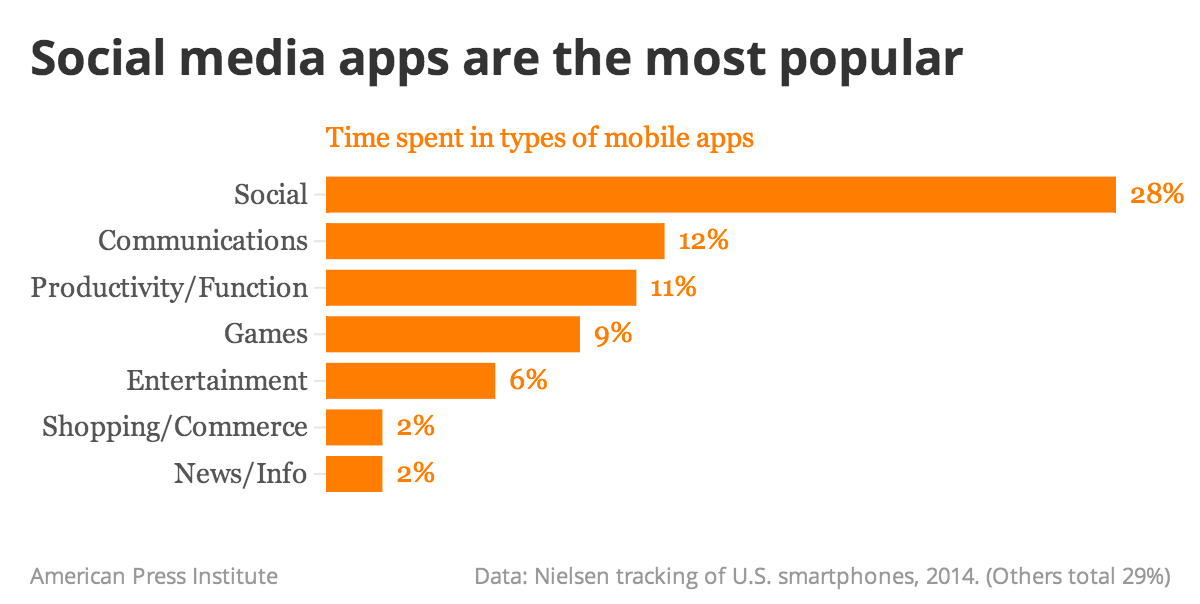
\includegraphics[scale=0.3]{figures/social-media-usage.png}
	\centering
	\caption{Οι χρήστες ξοδεύουν 14 φορές περισσότερο χρόνο χρησιμοποιώντας εφαρμογές όπως το \selectlanguage{english} \textit{facebook}\selectlanguage{greek}, έναντι εφαρμογών ενημέρωσης  (Πηγή: \cite{[AMP+14]})}
	\label{socialmediausage}
\end{figure}



\section{Αντικείμενο της διπλωματικής}

Εδώ αναφερόμαστε συγκεκριμένα στο τί θα κάνει η διπλωματική. Αναφέρουμε λεπτομερώς α) τα προβλήματα που θα λύσει (και που ήδη έχουν περιγραφεί γενικά στην προηγούμενη ενότητα), και β) πώς σκοπεύει να τα λύσει. 
Είναι σημαντικό κάποιος που θα διαβάσει την ενότητα αυτή να καταλάβει σε σημαντικό βαθμό τον σκοπό της διπλωματικής σας και τις τεχνικές δυσκολίες της, χωρίς να είναι αναγκαίο να δει όλα τα άλλα κεφάλαια. Η ενότητα αυτή θέλει πολύ προσοχή και καλύτερα να τη γράψετε αφού έχετε γράψει όλα τα υπόλοιπα κεφάλαια.

Το αντικείμενο με το οποίο καταπιάνεται το παρόν έργο, επικεντρώνεται στην σχεδίαση και την υλοποίηση μιας εφαρμογής, βασισμένη στην πρακτική ενεργοποίησης ενός ``\textit{πλήθους}'' ή μιας ομάδας, γνωστής και ως \textit{τακτική του πληθοπορισμού}. 

\subsection{Συνεισφορά}
Εδώ παραθέτουμε αριθμητικά συγκεκριμένες ενέργειες/λύσεις/μεθοδολογίες που παρουσιάζει η διπλωματική και λύνουν τα προβλήματα που υποσχεθήκαμε στην προηγούμενη ενότητα ότι θα λύσει η διπλωματική. Συνήθως η υποενότητα αυτή έχει την παρακάτω μορφή:

Η συνεισφορά της διπλωματικής συνοψίζεται ως εξής:
\begin{enumerate}
\item Μελετήθηκαν συστήματα κ.λ.π.
\item Υλοποιήθηκαν τρεις αλγόριθμοι υπολογισμού κ.λ.π.
\item Αξιολογήθηκε η επίδοση των αλγορίθμων και βρέθηκε ότι κ.λ.π.
\item Ενσωματώθηκαν οι αλγόριθμοι σε πρότυπο σύστημα κ.λ.π.
\item ...
\end{enumerate}


\section{Οργάνωση του τόμου}

Εδώ περιγράφουμε τα κεφάλαια της διπλωματικής: μία πρόταση για το τί θα έχει  κάθε κεφάλαιο.Συνήθως η ενότητα αυτή έχει την παρακάτω μορφή (δεν θα σας πάρει πάνω από μία μεγάλη παράγραφο):

Εργασίες σχετικές με το αντικείμενο της διπλωματικής παρουσιάζονται στο Κεφάλαιο \ref{chap2}. Το Κεφάλαιο \ref{chap3} συζητά θέματα μοντελοποίησης. Στο Κεφάλαιο \ref{chap4} αναπτύσσουμε κ.λ.π. 

Τονίζεται ότι η διάρθρωση του υπόλοιπου κειμένου (πλήθος και έκταση κεφαλαίων), καθώς και η ονομασία κάθε κεφαλαίου ή ενότητας σε αυτό το πρότυπο είναι εντελώς ενδεικτικά. Για την τελική οργάνωση του κειμένου σας, συμβουλευθείτε τον επιβλέποντα της εργασίας.


\chapter{Θεωρητικό και Τεχνολογικό υπόβαθρο}
\label{chap3}

<<<<<<< HEAD
Σε αυτό το κεφάλαιο θα γίνει μια εκτεταμένη ανάλυση όλων των βασικών εννοιών που θεμελιώνουν τόσο τη θεωρητική, όσο και την τεχνολογική βάση στην οποία στηρίζεται η διπλωματική εργασία. Καθώς το παρόν έργο αποτελεί συγκερασμό δύο επιστημονικών κλάδων (Κοινωνιολογία και Πληροφορική), είναι αναγκαία η διαίρεση αυτού του κεφαλαίου σε τρία μέρη. Στην ενότητα 2.3.1 αναλύεται το θεωρητικό μοντέλο και οι κοινωνιολογικές έννοιες που το συνιστούν. Η ενότητα 2.3.2 αναφέρεται σε σχετικές ερευνητικές προσπάθειες που έχουν προηγηθεί. Στο τρίτο μέρος παρατίθενται οι τεχνολογίες που χρησιμοποιήθηκαν για την ανάπτυξη της εφαρμογής (ενότητες 2.3.1-2.3.3), καθώς και άλλα σύγχρονα εργαλεία που χρησιμοποιήθηκαν (ενότητα 2.4).
=======
Σε αυτό το κεφάλαιο θα γίνει μια εκτεταμένη ανάλυση όλων των βασικών εννοιών που θεμελιώνουν τόσο τη θεωρητική, όσο και την τεχνολογική βάση στην οποία στηρίζεται η διπλωματική εργασία. Καθώς το παρόν έργο αποτελεί συγκερασμό δύο επιστημονικών κλάδων (Κοινωνιολογία και Πληροφορική), είναι αναγκαία η διαίρεση αυτού του κεφαλαίου σε ΠΟΣΕΣ ενότητες. Στην ενότητα 3.1 αναλύεται το θεωρητικό μοντέλο και οι κοινωνιολογικές έννοιες που το συνιστούν. Η ενότητα 3.2 αναφέρεται σε σχετικές ερευνητικές προσπάθειες που έχουν προηγηθεί. Τέλος, στην ενότητα 3.3 παρατίθενται τα σχετικά τεχνολογικά εργαλεία που χρησιμοποιήθηκαν.
>>>>>>> acacc83a12cc6f1be99d6d3fb0df8b0ed3fa708b

\section{Θεωρητικό Υπόβαθρο - Βασικές Έννοιες}

\subsection{Κοινωνικός Ρόλος των Σύγχρονων Εφαρμογών}
<<<<<<< HEAD
Πρωταρχικό ρόλο στην επιτυχία μιας εφαρμογής παίζει το κίνητρο με το οποίο αυτή εξασφαλίζει τη διαρκή ενασχόληση του χρήστη. Βασικό στοιχείο για να επιτευχθεί αυτό είναι o κοινωνικός ρόλος που επωμίζεται ο χρήστης εντός της εφαρμογής. Oι σημερινές εφαρμογές έχουν στρέψει την προσοχή γύρω από την κοινωνική προβολή και επιβολή, απομακρύνοντας την προσοχή από δημοσιεύσεις που αφορούν κοινωνικά δρώμενα, τεχνολογικά επιτεύγματα και γενικότερα τον συλλογικό βίο (βλ. Σχ. \ref{socialsharing}). Έτσι, παρατηρείται η προσκόλληση στα μέσα κοινωνικής δικτύωσης ως τρόπο άσκησης κοινωνικής επιρροής. Δημιουργούνται συνεπώς εγωκεντρικές τάσεις που τροφοδοτούν νέες ανάγκες και οδηγούν σε νέες ομοειδείς εφαρμογές. Τέτοια παραγείγματα είναι η ανάγκη για δημοτικότητα και κοινωνική αποδοχή \cite{[IND+16]} από τρίτους, η έντονη εμμονή με την προσωπική εικόνα στον ψηφιακό κόσμο και η ενίσχυση των απρόσωπων σχέσεων \cite{[JAR+18]}. 
=======
Πρωταρχικό ρόλο στην επιτυχία μιας εφαρμογής παίζει το κίνητρο με το οποίο αυτή εξαφαλίζει τη διαρκή ενασχόληση του χρήστη. Βασικό στοιχείο για να επιτευχθεί αυτό είναι o κοινωνικός ρόλος που επωμίζεται ο χρήστης εντός της εφαρμογής. Oι σημερινές εφαρμογές έχουν στρέψει την προσοχή γύρω από την κοινωνική προβολή και επιβολή, απομακρύνοντας την προσοχή από δημοσιεύσεις που αφορούν κοινωνικά δρώμενα, τεχνολογικά επιτεύγματα και γενικότερα τον συλλογικό βίο (βλ. Σχ. \ref{socialsharing}). Έτσι, παρατηρείται η προσκόλληση στα μέσα κοινωνικής δικτύωσης ως τρόπο άσκησης κοινωνικής επιρροής. Δημιουργούνται συνεπώς εγωκεντρικές τάσεις που τροφοδοτούν νέες ανάγκες και οδηγούν σε νέες ομοειδείς εφαρμογές. Τέτοια παραγείγματα είναι η ανάγκη για δημοτικότητα και κοινωνική αποδοχή \cite{[IND+16]} από τρίτους, η έντονη εμμονή με την προσωπική εικόνα στον ψηφιακό κόσμο και η ενίσχυση των απρόσωπων σχέσεων \cite{[JAR+18]}. 
>>>>>>> acacc83a12cc6f1be99d6d3fb0df8b0ed3fa708b

\begin{figure}[H]
    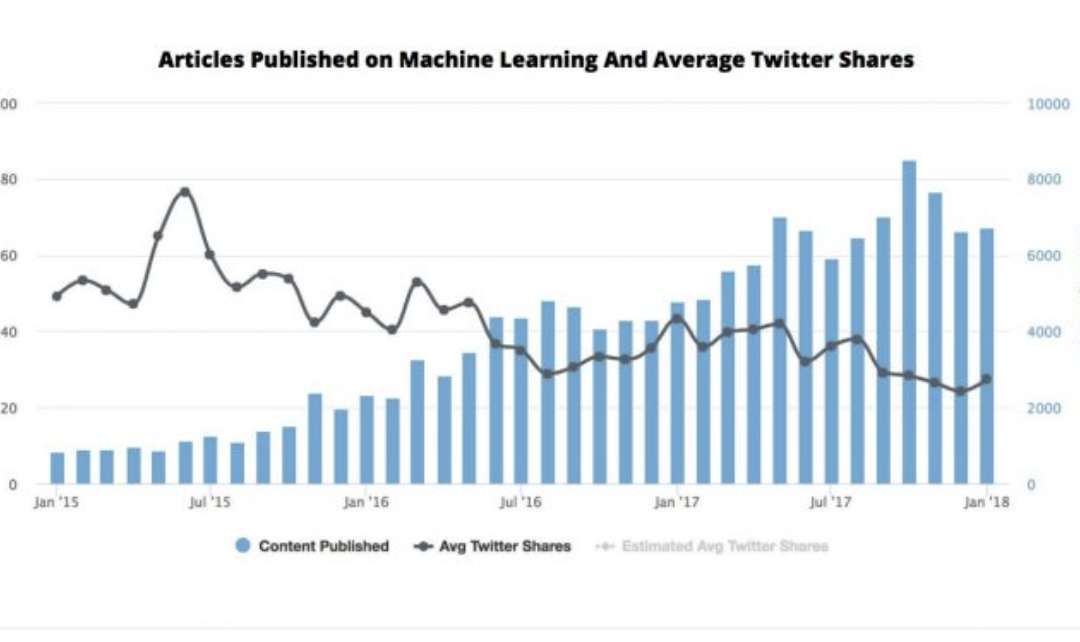
\includegraphics[scale=0.3]{figures/social-share-has-decreased.png}
    \centering
    \caption{Η δημοσιεύσεις κοινωνικών γεγονότων έχουν υποχωρήσει αισθητά. (Πηγή: \cite{[VEN+18]})}
    \label{socialsharing}
\end{figure}


Προκειμένου να επαναπροσδιοριστεί ο ρόλος των εφαρμογών, είναι απαραίτητο να αναθεωρηθούν τα κίνητρα με τα οποία αυτές κεντρίζουν το ενδιαφέρον του χρήστη. Η κοινωνική επίδειξη, να αντικατασταθεί με την κοινωνική συνεισφορά, ενώ η απομόνωση θα πρέπει να δώσει τη θέση της στην επανένταξη του ατόμου στο κοινωνικό σύνολο. Η ενημέρωση μέσω των εφαρμογών, οφείλει να έχει κοινωνικό χαρακτήρα και όχι να προβάλλει την προσωπική ζωή, ή να ωθεί σε κοινωνικά σύνδρομα τους χρήστες \cite{[BBC+18]}. 

\subsection{Ανάγκη της Κοινωνικής Προσφοράς}
Έχοντας υπόψη τα παραπάνω, καταλήγει κανείς εύκολα στο συμπέρασμα ότι υπάρχει μεγάλη ανάγκη να επανασυνδεθεί ο ρόλος των κοινωνικών εφαρμογών με την συνεισφορά για το κοινό συμφέρον. Αν και ζούμε σε μία εποχή όπου η τεχνολογία προχωράει με αλματώδεις ρυθμούς, ελάχιστο είναι το ποσοστό του συνόλου που γνωρίζει για τα επιτεύγματα των συγχρόνων του στους διάφορους επιστημονικόυς τομείς. Ακόμη κι αν το άτομο εκδηλώνει ενδιαφέρον, είναι δύσκολο να ενημερωθεί όταν όλες οι θεματικές περιστρέφονται γύρω από την προσωπική ζωή. Προκύπτει, λοιπόν μια νέα ανάγκη για κινητοποίηση του χρήστη να αλληλεπιδράσει με το κοινωνικό σύνολο. Αυτό είναι εφικτό χρησιμοποιώντας τις δυνατότητες των ήδη γνωστών εφαρμογών, αυτή τη φορά με σκοπό την ενημέρωση για γεγονότα που αφορούν την ευρύτερη πολιτισμική κοινότητα. 

\subsection{Η Έννοια του Πληθοπορισμού}
%Εδώ γράφουμε σύντομα τις τεχνικές/μεθοδολογίες/μοντέλα που πιθανά θα χρησιμοποιήσει η διπλωματική και είναι αναγκαία η κατανόησή τους από τον αναγνώστη πριν από την παρουσίαση της ανάλυσης και σχεδίασης του συστήματος. Πρόκειται για τεχνικές/μεθοδολογίες/μοντέλα που έχουν προταθεί από άλλους και δεν είναι πρωτότυπη δουλειά της διπλωματικής. Μετά βάζουμε μία ενότητα για κάθε τεχνική/μεθοδολογία/μοντέλο, όπου και δίνουμε λεπτομερή περιγραφή.
<<<<<<< HEAD
Συνδυάζοντας τη δύναμη της συλλογικής προσφοράς με την τεχνολογία και τεχνογνωσία που είναι διαθέσιμη σήμερα, η ενημέρωση μπορεί να πάρει νέα διάσταση. Με στοχευμένο προσανατολισμό της κοινωνικής διάθεσης για δράση προς μία συγκεκριμένη κατεύθυνση, η κοινωνία μπορεί να στρατολογήσει τα ίδια τα μέλη της προκειμένου να προάγει τις τεχνολογικές, πολιτισμικές και κοινωνικές εκδηλώσεις, να συντονίσει την πληροφορία και να ενημερώσει το σύνολο. Σύμφωνα με τη \selectlanguage{english}\textit{New York Times}\selectlanguage{greek}, χάρις στην αυξανόμενη συνδεσιμότητα μέσω του διαδικτύου, εκατομμύρια ανθρώπων μπορούν να συνεισφέρουν ιδέες και πληροφορίες για προβλήματα οποιασδήποτε μορφής. Η πρακτική της συμμετοχής ενός «πλήθους» ή μιας ομάδας για έναν κοινο στόχο ή επίλυση κοινών προβλημάτων, με την επιστράτευση της τεχνολογίας ως διαύλου επικοινωνίας ονομάζεται \textit{πληθοπορισμός} (\selectlanguage{english}\textit{crowdsourcing})\selectlanguage{greek} \cite{[CSW+18]}.
=======
Συνδυάζοντας τη δύναμη της συλλογικής προσφοράς με την τεχνολογία και τεχνογνωσία που είναι διαθέσιμη σήμερα, η ενημέρωση μπορεί να πάρει νέα διάσταση. Με στοχευμένο προσανατολισμό της κοινωνικής διάθεσης για δράση προς μία συγκεκριμένη κατεύθυνση, η κοινωνία μπορεί να στρατολογήσει τα ίδια τα μέλη της προκειμένου να προάγει τις τεχνολογικές, πολιτισμικές και κοινωνικές εκδηλώσεις, να συντονίσει την πληροφορία και να ενημερώσει το σύνολο. Σύμφωνα με τη \selectlanguage{english}\textit{New York Times}\selectlanguage{greek}, χάρις στην αυξανόμενη συνδεσιμότητα μέσω του διαδικτύου, εκατομμύρια ανθρώπων μπορούν να συνεισφέρουν ιδέες και πληροφορίες για προβλήματα οποιασδήποτε μορφής. Η πρακτική της συμμετοχής ενός «πλήθους» ή μιας ομάδας για έναν κοινο στόχο ή επίλυση κοινών προβλημάτων, με την επιστράτευση της τεχνολογίας ως διαύλου επικοινωνίας ονομάζεται \textit{πληθοπορισμός} (\selectlanguage{english}\textit{Crowdsourcing})\selectlanguage{greek} \cite{[CSW+18]}.
>>>>>>> acacc83a12cc6f1be99d6d3fb0df8b0ed3fa708b

\subsubsection{Εφαρμογές του Πληθοπορισμού}
Τα πεδία στα οποία μπορεί να αξιοποιηθεί η τεχνική του πληθοποριμού είναι αμέτρητα. Ο,τιδήποτε μπορεί να αποκτήσει συνεργατικό χαρακτήρα. Αναφορικά, παρατίθενται μερικοί κλάδοι όπου ανθεί η τεχνική αυτή:
\begin{description}[font=$\bullet$~\normalfont\color{black}]
\item [Εκπαίδευση]
\item [Οικονομία]
\item [Επιστήμη και Υγεία]
\item [ΙΤ]
\item [Διαφήμιση]
\item [Επιχειρηματικότητα]
<<<<<<< HEAD
\item [Κοινωνικές Εκδηλώσεις και \selectlanguage{english}\textit{NGO}\selectlanguage{greek}]
=======
\item [Κοινωνικές Εκδηλώσεις και ΜΚΟ]
>>>>>>> acacc83a12cc6f1be99d6d3fb0df8b0ed3fa708b
\end{description}

\subsubsection{Μοντέλο Πληθοπορισμού στην Εφαρμογή}
Η εφαρμογή σκοπεύει να χρησιμοποιήσει την πρακτική του πληθοπορισμού για να συγκεντρώσει πληροφορίες σχετικές με πολιτισμικές και κοινωνικές εκδηλώσεις. Οι χρήστες θα έχουν τη δυνατότητα να αξιολογούν τα πάντα γύρω από ένα γεγονός. Θα είναι δυνατή η ενημέρωση για τυχόν αλλαγές της ώρας και του τόπου, για προβλήματα που μπορεί να δυσκολέψουν την διεξαγωγή της εκδήλωσης, ή ιδέες για την καλυτέρευση αυτής. Το σημαντικό στοιχείο όλων των παραπάνω είναι πως θα μπορούν να γίνουν σε πραγματικό χρόνο. Αυτό θα έχει σαν αποτέλεσμα την καλύτερη αλληλεπίδραση μεταξύ συμμετεχόντων και διοργανωτών, την αποφυγή προβλημάτων και παρανοήσεων και την καλύτερη ενημέρωση του πλήθους. Διοργανωτές και συμμετέχοντες, θα μπορούν να εκφράσουν τη γνώμη τους, όλοι ως χρήστες της εφαρμογής. Η πληροφορία θα επικαιροποιείται διαρκώς από όσους παρευρίσκονται ήδη εκεί και θα διαδίδεται σε όσους μέχρι τώρα την αγνοούσαν.Το παραπάνω μοντέλο υλοποιειται μέσω ενός συστήματος μηνυμάτων μεταξύ των χρηστών. 

\section{Σχετικές Ερευνητικές Προσπάθειες και Πρότυπα}
Αν και το παρόν έργο αποτελεί προσωπική πρωτοβουλία, η ιδέα της διπλωματικής έχει κάποιες επιρροές και από άλλα παράλληλα έργα στον ίδιο τομέα. Τέτοια έργα είναι το \selectlanguage{english}\textit{WITHcrowd}\selectlanguage{greek} της ερευνητικής ομάδας του εργαστηρίου Ευφυών Συστημάτων (\selectlanguage{english}\textit{ISLAB}\selectlanguage{greek}) του Εθνικού Μετσόβιου  Πολυτεχνείου, που αποτελεί μέρος του ευρωπαϊκού προγράμματος \selectlanguage{english}\textit{WITH}\selectlanguage{greek}. Το έργο αυτό αποτέλεσε πηγή έμπνευσης για το κομμάτι του πληθοπορισμού στην εφαρμογή της παρούσας εργασίας. Χρησιμοποιήθηκαν επίσης to πρότυπo ανοιχού κώδικα \selectlanguage{english}\textit{Foursquare API}\selectlanguage{greek}, και οι διεπαφές αυτού,  \selectlanguage{english}\textit{Foursquare Autocomplete}\selectlanguage{greek} και \selectlanguage{english}\textit{Foursquare Places}\selectlanguage{greek}. Συνολικά, η εφαρμογή είναι μια καινοτομία η οποία προσπαθεί να στρέψει ήδη υπάρχουσες πρακτικές προς μια νέα κατεύθυνση, χρησιμοποιώντας τις σύγχρονη τεχνογνωσία για έναν πρωτοποριακό σκοπό.   

\subsection{\selectlanguage{english}WITHcrowd}
<<<<<<< HEAD
To \selectlanguage{english}WITHcrowd \cite{[WIT+18]}\selectlanguage{greek} είναι μια πρωτοβουλία της ευρωπαϊκής κοινότητας για τη συλλογή και ταξινόμηση δεδομένων πολιτισμικού περιεχομένου. Αποτελείται από μία πλατφόρμα που εκθέτει τις διεπαφές (ΑΡΙ) διαφόρων πυλών (\selectlanguage{english}portals)\selectlanguage{greek} και ψηφιακών αποθηκών (\selectlanguage{english}repositories)\selectlanguage{greek}. Eπιτρέπει στους χρήστες την αναζήτηση ψηφιακού περιεχομένου από μια σειρά διαφορετικών και ανεξάρτητων αποθετηρίων και βάσεων δεδομένων από ένα ενιαίο σημείο πρόσβασης. Τα αποθετήρια που μπορούν να αναζητηθούν περιλαμβάνουν μεταξύ άλλων την \selectlanguage{english}Europeana,\selectlanguage{greek} την Ψηφιακή Δημόσια Βιβλιοθήκη της Αμερικής, το \selectlanguage{english}YouTube,\selectlanguage{greek} το Μουσείο \selectlanguage{english}Rijks,\selectlanguage{greek} την Εθνική Βιβλιοθήκη της Αυστραλίας και την Ψηφιακή Νέα Ζηλανδία. Όλη η δύναμη της πλατφόρμας συγκεντρώνεται στο γεγονός ότι ο χρήστης είναι υπεύθυνος για την επίτευξη του στόχου του προγράμματος. Αυτή την πρακτική επιχειρεί να υιοθετήσει η εφαρμογή που θα αναλυθεί στα επόμενα κεφάλαια. 

\subsection{\selectlanguage{english}Foursquare API}
Το \selectlanguage{english}\textit{Foursquare API} \cite{[4SQ+18]}\selectlanguage{greek} είναι η διεπαφή της εφαρμογής \selectlanguage{english}\textit{Foursquare}\selectlanguage{greek} και παρέχεται στην κοινότητα της πληροφορικής δωρεάν. Δίνει τη δυνατότητα στους προγραμματιστές να χρησιμοποιήσουν δεδομένα που αφορούν τελικά σημεία (\selectlanguage{english}endpoints)\selectlanguage{greek} σε Ενιαίους Εντοπιστές Πόρων (\selectlanguage{english}URLs)\selectlanguage{greek}, όπως τα στοιχεία μιας υπηρεσίας (πχ. τοποθεσία, πληροφορίες επικοινωνίας, διεύθυνση, όνομα, κατηγορία, ώρες λειτουργίας, παροχές κλπ).
=======
To \selectlanguage{english}WITHcrowd\cite{[WIT+18]}\selectlanguage{greek} είναι μια πρωτοβουλία της ευρωπαϊκής κοινότητας για τη συλλογή και ταξινόμηση δεδομένων πολιτισμικού περιεχομένου. Αποτελείται από μία πλατφόρμα που εκθέτει τις διεπαφές (ΑΡΙ) διαφόρων πυλών (\selectlanguage{english}portals)\selectlanguage{greek} και ψηφιακών αποθηκών (\selectlanguage{english}repositories)\selectlanguage{greek}. Eπιτρέπει στους χρήστες την αναζήτηση ψηφιακού περιεχομένου από μια σειρά διαφορετικών και ανεξάρτητων αποθετηρίων και βάσεων δεδομένων από ένα ενιαίο σημείο πρόσβασης. Τα αποθετήρια που μπορούν να αναζητηθούν περιλαμβάνουν μεταξύ άλλων την \selectlanguage{english}Europeana,\selectlanguage{greek} την Ψηφιακή Δημόσια Βιβλιοθήκη της Αμερικής, το \selectlanguage{english}YouTube,\selectlanguage{greek} το Μουσείο \selectlanguage{english}Rijks,\selectlanguage{greek} την Εθνική Βιβλιοθήκη της Αυστραλίας και την Ψηφιακή Νέα Ζηλανδία. Όλη η δύναμη της πλατφόρμας συγκεντρώνεται στο γεγονός ότι ο χρήστης είναι υπεύθυνος για την επίτευξη του στόχου του προγράμματος. Αυτή την πρακτική επιχειρεί να υιοθετήσει η εφαρμογή που θα αναλυθεί στα επόμενα κεφάλαια. 

\subsection{\selectlanguage{english}Foursquare API}
Το \selectlanguage{english}\textit{Foursquare API}\cite{[4SQ+18]}\selectlanguage{greek} είναι η διεπαφή της εφαρμογής \selectlanguage{english}\textit{Foursquare}\selectlanguage{greek} και παρέχεται στην κοινότητα της πληροφορικής δωρεάν. Δίνει τη δυνατότητα στους προγραμματιστές να χρησιμοποιήσουν δεδομένα που αφορούν τελικά σημεία (\selectlanguage{english}endpoints)\selectlanguage{greek} σε Ενιαίους Εντοπιστές Πόρων (\selectlanguage{english}URLs)\selectlanguage{greek}, όπως τα στοιχεία μιας υπηρεσίας (πχ. τοποθεσία, πληροφορίες επικοινωνίας, διεύθυνση, όνομα, κατηγορία, ώρες λειτουργίας, παροχές κλπ).
>>>>>>> acacc83a12cc6f1be99d6d3fb0df8b0ed3fa708b

To \selectlanguage{english}\textit{Foursquare}\selectlanguage{greek} έφερε την επανάσταση στα μέσα κοινωνικής δικτύωσης με την καινοτομία του ``\textit{\selectlanguage{english}check in}''.  Η λειτουργία της εφαρμογής \selectlanguage{english}Foursquare\selectlanguage{greek} συνοψίζεται στην αξιολόγηση και άσκηση κριτικής σε κέντρα διασκέδασης, εστιατόρια και χώρους ψυχαγωγίας. Ο χρήστης δημοσιεύει την τοποθεσία του κάνοντας \selectlanguage{english}check in\selectlanguage{greek} και ενημερώνει τους υπόλοιπους χρήστες-φίλους του. Η εφαρμογή που θα υλοποιηθεί κάνει μια απόπειρα να διοχετεύσει την πληροφορία σε αντίστοιχα μέρη πολιτισμικού ή κοινωνικού περιεχομένου και να την αξιοποιήσει για την αξιολόγησή τους.


\section{\selectlanguage{greek}Τεχνολογικό υπόβαθρο - Βασικές Έννοιες}
Στη συνέχεια θα γίνει μια εισαγωγή στις τεχνολογίες και τα εργαλεία προγραμματισμού. Έπειτα ακολουθεί η ανάλυση των σύγχρονων τεχνολογικών μέσων που αποτελούν τη βάση των μεθόδων και μοντέλων που χρησιμοποιήθηκαν στην υλοποίηση της εφαρμογής. 

Όταν ένας προγραμματιστής αναπτύσσει μία εφαρμογή, καλείται να προσδιορίσει τρία πράγματα:
\begin{enumerate}
\item Tην φύση της εφαρμογής - αν θα τρέχει σε φυλλομετρητή (\selectlanguage{english}Web Application)\selectlanguage{greek} ή αν θα είναι μητρική (\selectlanguage{english}Native Application)\selectlanguage{greek}.
\item Την γλώσσα στην οποία θα αναπτύξει την εφαρμογή (\selectlanguage{english}Programming Language)\selectlanguage{greek}
\item Την πλατφόρμα λογισμικού στην οποία θα υλοποιήσει την εφαρμογή (\selectlanguage{english}\textit{SDK})\selectlanguage{greek}
\end{enumerate}

\subsection{Είδη Γλωσσών Προγραμματισμού}
Πρωτού μιλήσουμε για τα είδη των σύγχρονων εφαρμογών, είναι απαραίτητο να αναλύσουμε τις κατηγορίες των αντίστοιχων γλωσσών και τις διακρίσεις μεταξύ αυτών. Μια γλώσσα μπορεί να ανήκει σε μία από τις παρακάτω κατηγορίες:
\begin{description}[font=$\bullet$~\normalfont\color{black}]
\item [Μετταγλωτισμένες ή Μητρικές γλώσσες (\selectlanguage{english}Compiled or Native Languages)]\selectlanguage{greek}
\item [Διαχειριζόμενες Γλώσσες (\selectlanguage{english}Managed Languages)]\selectlanguage{greek}
\item [Δυναμικές Γλώσσες (\selectlanguage{english}Dynamic Languages)]\selectlanguage{greek}
<<<<<<< HEAD
\end{description}Η μητρική γλώσσα (\selectlanguage{english}native language)\selectlanguage{greek} είναι μια γλώσσα που μπορεί να τρέξει στην πλατφόρμα του λειτουργικού συστήματος χωρίς να μετατραπεί σε άλλη μορφή κώδικα από τους μεταγλωττιστές (\selectlanguage{english}compilers)\selectlanguage{greek}. Αυτό σημαίνει πως η υλοποίησή της συνοψίζεται κυρίως στη χρήση μεταγλωττιστών, οι οποίοι είναι υπεύθυνοι για τη μετατροπή του κώδικα από γλώσσα μηχανής σε πηγαίο κώδικα (πχ. \selectlanguage{english}\textit{C++, C\#, Java, Swift})\selectlanguage{greek}. Η διαχειριζόμενη γλώσσα (\selectlanguage{english}managed language)\selectlanguage{greek} είναι μια γλώσσα που πρέπει να μετατραπεί ή να ερμηνευτεί πριν να εκτελεστεί στην πλατφόρμα (πχ.\selectlanguage{english} \textit{.NET})\selectlanguage{greek}. Σε αυτή την περίπτωση, ο κώδικας θα εκτελεστεί υπό τη διαχείριση μιας εικονικής μηχανής γλώσσας κοινού χρόνου εκτέλεσης ή, όπως είναι γνωστή,\selectlanguage{english} \textit{CLR}\selectlanguage{greek} \cite{[STR+09],[DEV+03]} (βλ. Σχ. \ref{clr}). Η δυναμική γλώσσα προγραμματισμού (\selectlanguage{english}dynamic language)\selectlanguage{greek} είναι μια κλάση αποτελούμενη από γλώσσες υψηλού επιπέδου (\selectlanguage{english}high-level programming languages)\selectlanguage{greek}, οι οποίες έχουν την ιδιότητα να εκτελούν πολλαπλές εντολές κατά το στάδιο της εκτέλεσης, σε αντίθεση με τις υπόλοιπες γλώσσες που εκτελούν εντολές στο στάδιο μεταγλώττισης  (πχ.\selectlanguage{english} \textit{Python, JavaScript, PHP, Ruby, MATLAB, Elixir})\selectlanguage{greek} \cite{[MIC05], [ADV09]}.

\begin{figure}[H]
    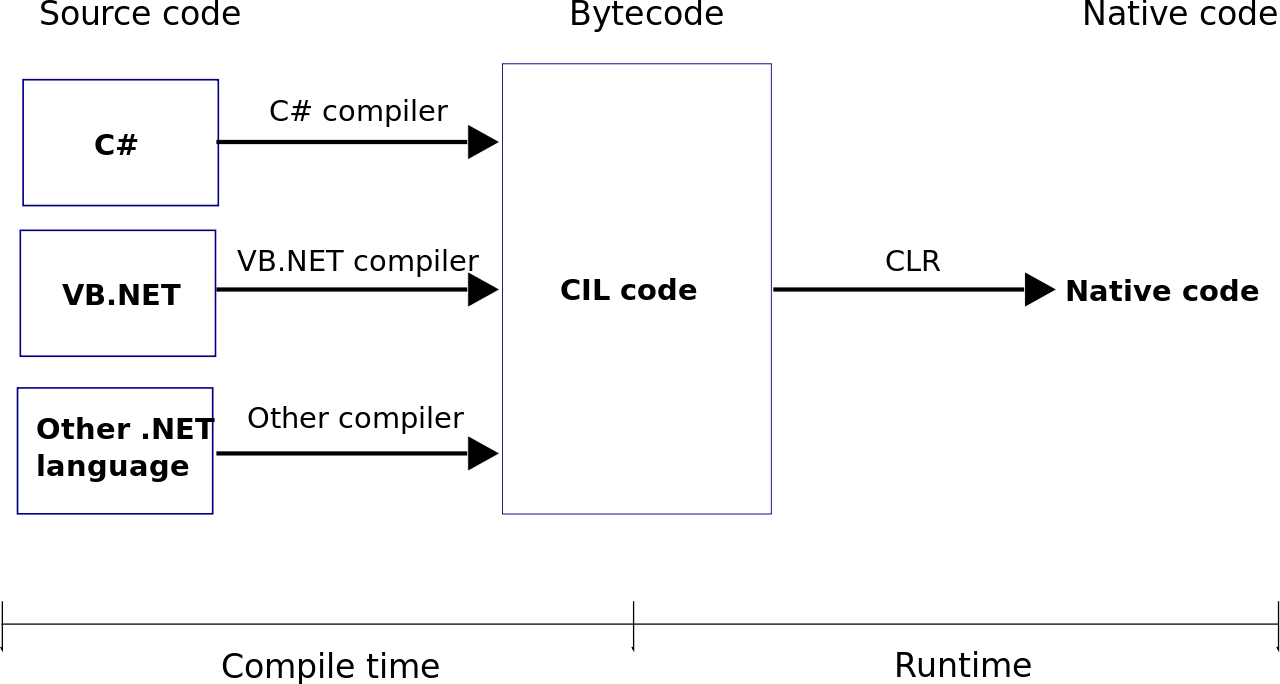
\includegraphics[scale=0.3]{figures/clr-converts-language-to-native-code.png}
    \centering
    \caption{Το \selectlanguage{english}CLR\selectlanguage{greek} μετατρέπει \selectlanguage{english}CIL\selectlanguage{greek} σε μητρικό κώδικα.}
    \label{clr}
\end{figure}
=======
\end{description}Η μητρική γλώσσα (\selectlanguage{english}native language)\selectlanguage{greek} είναι μια γλώσσα που μπορεί να τρέξει στην πλατφόρμα του λειτουργικού συστήματος χωρίς να μετατραπεί σε άλλη μορφή κώδικα από τους μεταγλωττιστές (\selectlanguage{english}compilers)\selectlanguage{greek}. Αυτό σημαίνει πως η υλοποίησή της συνοψίζεται κυρίως στη χρήση μεταγλωττιστών (\selectlanguage{english}compilers)\selectlanguage{greek}, οι οποίοι είναι υπεύθυνοι για τη μετατροπή του κώδικα από γλώσσα μηχανής σε πηγαίο κώδικα (πχ. \selectlanguage{english}\textit{C++, C\#, Java, Swift})\selectlanguage{greek}. Η διαχειριζόμενη γλώσσα (\selectlanguage{english}managed language)\selectlanguage{greek} είναι μια γλώσσα που πρέπει να μετατραπεί ή να ερμηνευτεί πριν να εκτελεστεί στην πλατφόρμα (πχ.\selectlanguage{english} \textit{.NET})\selectlanguage{greek}. Σε αυτή την περίπτωση, ο κώδικας θα εκτελεστεί υπό τη διαχείριση μιας εικονικής μηχανής γλώσσας κοινού χρόνου εκτέλεσης ή, όπως είναι γνωστή,\selectlanguage{english} \textit{CLR}\selectlanguage{greek} \cite{[STR+09],[DEV+03]}. Η δυναμική γλώσσα προγραμματισμού (\selectlanguage{english}dynamic language)\selectlanguage{greek} είναι μια κλάση αποτελούμενη από γλώσσες υψηλού επιπέδου (\selectlanguage{english}high-level programming languages)\selectlanguage{greek}, οι οποίες έχουν την ιδιότητα να εκτελούν πολλαπλές εντολές κατά το στάδιο της εκτέλεσης, σε αντίθεση με τις υπόλοιπες γλώσσες που εκτελούν εντολές στο στάδιο μεταγλώττισης  (πχ.\selectlanguage{english} \textit{Python, JavaScript, PHP, Ruby, MATLAB, Elixir})\selectlanguage{greek} \cite{[MIC05], [ADV09]}.
>>>>>>> acacc83a12cc6f1be99d6d3fb0df8b0ed3fa708b

Οι γλώσσες υψηλού επιπέδου, όπως η \selectlanguage{english}Python\selectlanguage{greek} και η \selectlanguage{english}Ruby\selectlanguage{greek}, έχουν αποκτήσει μεγάλη απήχηση τα τελευταία χρόνια. Για πολλούς, αποτελούν τη νέα γεννιά γλωσσών προγραμματισμού. Ωστόσο οι ρίζες τους ανατρέχουν στις αρχές της δεκαετίας του '50, με την γέννηση της \selectlanguage{english}Lisp\selectlanguage{greek} της πρώτης γλώσσας υψηλού επιπέδου. Πλέον, οι δυναμικές γλώσσες συναντόνται τόσο σε πραγματικά διαδικτυακά συστήματα, όσο και σε εφαρμογές που πριν κυριαρχούσαν οι στατικές γλώσσες προγραμματισμού \cite{[ADV09]}.

Εμείς θα επικεντρωθούμε στην πρώτη κατηγορία, των μητρικών ή αλλιώς μεταφρασμένων γλωσσών προγραμματισμού. Το πλεονέκτημα χρήσης μητρικού κώδικα (\selectlanguage{english}native code\selectlanguage{greek}) βρίσκεται στο γεγονός ότι προγράμματα σε τέτοιες γλώσσες είναι γρηγορότερα, χάρις τον μειωμένο χρόνο επιβάρυνσης (\selectlanguage{english}overhead)\selectlanguage{greek} της διαδικασίας μετάφρασης. Αυτό οφείλεται στην ιδιότητά τους να μεταγλωττίζονται κατά το χρόνο μεταγλώττισης και όχι κατά το χρόνο εκτέλεσης, όπως συμβαίνει με άλλα προγράμματα.

Οι γλώσσες χαμηλού επιπέδου (\selectlanguage{english}low-level programming languages)\selectlanguage{greek} είναι δομημένες έτσι ώστε να υφίστανται την τυπική μεταγλώττιση, ειδικά όταν η αποτελεσματικότητα είναι πρωταρχικό μέλημα, έναντι της μεταγλώττισης που υποστηρίζει πολλές πλατφόρμες (\selectlanguage{english}cross-platform)\selectlanguage{greek}. Για αυτές τις γλώσσες, υπάρχουν περισσότερες ένα-προς-ένα αντιστοιχίες ανάμεσα στο προγραμματισμένο κώδικα και τις λειτουργίες υλικού που εκτελούνται σε κώδικα μηχανής, καθιστώντας ευκολότερο για τους προγραμματιστές τον έλεγχο χρήσης της κεντρικής μονάδας επεξεργασίας και μνήμης με λεπτομέρεια. 
<<<<<<< HEAD
Με κάποια προσπάθεια, είναι πάντα δυνατή η σύνταξη μεταγλωττιστών ακόμα και για παραδοσιακά ερμηνευμένες γλώσσες. Για παράδειγμα, η\selectlanguage{english} Common lisp\selectlanguage{greek} μπορεί να μεταγλωττιστεί σε \selectlanguage{english}Java bytecode\selectlanguage{greek} (στη συνέχεια ερμηνεύεται από την εικονική μηχανή\selectlanguage{english} Java\selectlanguage{greek}), σε κώδικα\selectlanguage{english} C\selectlanguage{greek} (στη συνέχεια, μεταγλωττίζεται στον εγγενή κώδικα μηχανής) ή απευθείας σε εγγενή κώδικα. Οι γλώσσες προγραμματισμού που υποστηρίζουν πολλαπλούς στόχους σύνταξης δίνουν μεγαλύτερο έλεγχο στους προγραμματιστές για να επιλέξουν είτε ταχύτητα εκτέλεσης είτε συμβατότητα μεταξύ πολλαπλών πλατφόρμων \cite{[SQA+07]}.

\clearpage
=======
Με κάποια προσπάθεια, είναι πάντα δυνατή η σύνταξη μεταγλωττιστών ακόμα και για παραδοσιακά ερμηνευμένες γλώσσες. Για παράδειγμα, η\selectlanguage{english} Common lisp\selectlanguage{greek} μπορεί να μεταγλωττιστεί σε \selectlanguage{english}Java bytecode\selectlanguage{greek} (στη συνέχεια ερμηνεύεται από την εικονική μηχανή\selectlanguage{english} Java\selectlanguage{greek}), σε κώδικα\selectlanguage{english} C\selectlanguage{greek} (στη συνέχεια, μεταγλωττίζεται στον εγγενή κώδικα μηχανής) ή απευθείας σε εγγενή κώδικα. Οι γλώσσες προγραμματισμού που υποστηρίζουν πολλαπλούς στόχους σύνταξης δίνουν μεγαλύτερο έλεγχο στους προγραμματιστές για να επιλέξουν είτε ταχύτητα εκτέλεσης είτε συμβατότητα μεταξύ πλατφόρμων \cite{[SQA+07]}.
>>>>>>> acacc83a12cc6f1be99d6d3fb0df8b0ed3fa708b

\selectlanguage{english}
\begin{lstlisting}[language=Python, caption=\selectlanguage{greek}Παράδειγμα κώδικα σε \selectlanguage{english}Python]
import numpy as np
 
def incmatrix(genl1,genl2):
    m = len(genl1)
    n = len(genl2)
    M = None #to become the incidence matrix
    VT = np.zeros((n*m,1), int)  #dummy variable
 
    #compute the bitwise xor matrix
    M1 = bitxormatrix(genl1)
    M2 = np.triu(bitxormatrix(genl2),1) 
 
    for i in range(m-1):
        for j in range(i+1, m):
            [r,c] = np.where(M2 == M1[i,j])
            for k in range(len(r)):
                VT[(i)*n + r[k]] = 1;
                VT[(i)*n + c[k]] = 1;
                VT[(j)*n + r[k]] = 1;
                VT[(j)*n + c[k]] = 1;
 
                if M is None:
                    M = np.copy(VT)
                else:
                    M = np.concatenate((M, VT), 1)
 
                VT = np.zeros((n*m,1), int)
 
    return M
\end{lstlisting}

\selectlanguage{greek}
\subsection{Μητρικές Γλώσσες Προγραμματισμού (\selectlanguage{english}Native Programming Languages)}
\selectlanguage{greek}
%Μιλάμε για τις δυνατοτητες τους και τα μειονεκτηματα τους (αναφορα σε σχετικα αρθρα, παραθεση δειγματος κωδικα και παραθεση διαγραμματων με την πτωση της χρησης τους)
Έχοντας προσδιορίσει τις κατηγορίες γλωσσών προγραμματισμού, μπορεί κανείς επομένως να αντιληφθεί την ανάγκη των μητρικών ή αλλιώς μεταγλωττισμένων γλωσσών για την ανάπτυξη εφαρμογών σε συγκεκριμένες πλατφόρμες. Αυτές οι γλώσσες είναι κατά κύριο λόγο σχεδιασμένες να τρέχουν σε μια ορισμένη πλατφόρμα για καλύτερη απόδοση και ευκολότερο σχεδιασμό. Τέτοιες γλώσσες που χρησιμοποιούνται σήμερα στις εφαρμογές κινητών συσκευών είναι η \selectlanguage{english}Swift\selectlanguage{greek} και η \selectlanguage{english}Java\selectlanguage{greek}. Η πρώτη χρησιμοποιείται για την υλοποίηση εφαρμογών σε \selectlanguage{english}iOS\selectlanguage{greek} πλατφόρμες, ενώ η δεύτερη για την ανάπτυξη εφαρμογών που τρέχουν σε \selectlanguage{english}Android\selectlanguage{greek} πλατφόρμες.

\subsubsection{\selectlanguage{english}Swift - iOS Development}
\selectlanguage{greek}
Η \selectlanguage{english}\textit{Swift}\selectlanguage{greek} είναι μια μεταγλωττισμένη, γενικού σκοπού, πολυπαραδειγματική γλώσσα προγραμματισμού που έχει αναπτυχθεί από την \selectlanguage{english}\textit{Apple Inc.}\selectlanguage{greek} για τα προϊόντα τις ίδιας εταιρείας (\selectlanguage{english}\textit{iOS, macOS, watchOS, tvOS}\selectlanguage{greek}). Είναι σχεδιασμένη ώστε να δουλεύει με το \textit{\selectlanguage{english}XCode IDE\selectlanguage{greek}} και χρησιμοποιείται από την κοινότητα των \selectlanguage{english}iOS developers\selectlanguage{greek} για ανάπτυξη \selectlanguage{english}iOS\selectlanguage{greek} εφαρμογών, υποστηριζόμενων από τις πλατφόρμες και τα προϊόντα \selectlanguage{english}Apple\selectlanguage{greek} \cite{[SWIFT1+16]}.

Τα πρώτα βήματα για την δημιουργία της \selectlanguage{english}Swift\selectlanguage{greek} ξεκίνησαν υπό την καθοδήγηση του \selectlanguage{english}C.~Lattner\selectlanguage{greek}, εντός της \selectlanguage{english}Apple\selectlanguage{greek}. Με επιρροές από γλώσσες όπως οι \selectlanguage{english}\textit{Objective-C, Rust, Haskell, C\#}\selectlanguage{greek} και αρκετές ακόμη \cite{[SWIFT2+14]}, η \selectlanguage{english}Swift\selectlanguage{greek} ήρθε στο προσκήνιο επίσημα για πρώτη φορά στο Παγκόσμιο Συνέδριο Προγραμματιστών (\selectlanguage{english}WWDC\selectlanguage{greek}) τον Ιούνιο του 2014 \cite{[SWIFT3+14]}. 

Βασικά γνωρίσματα αυτής της γλώσσας είναι η αντικειμενοστρέφεια (\selectlanguage{english}\textit{OO} language\selectlanguage{greek}), και η απλουστευμένες δομές. Η \selectlanguage{english}Swift\selectlanguage{greek} βασίζεται σε θεωρητικές έννοιες των μοντέρνων γλωσσών προγραμματισμού και προσπαθεί να παρουσιάσει μια απλούστερη συντακτική προσέγγιση \cite{[SWIFT4], [SWIFT5]}. 

\selectlanguage{english}
\begin{lstlisting}[language=Swift, caption=\selectlanguage{greek}Παράδειγμα κώδικα σε \selectlanguage{english}Swift]
    import UIKit
    import AVFoundation
    
class ViewController: UIViewController {
    
    @IBOutlet weak var darkBlueBG: UIImageView!
    @IBOutlet weak var powerBtn: UIButton!
    @IBOutlet weak var cloudHolder: UIView!
    @IBOutlet weak var rocket: UIImageView!
    @IBOutlet weak var hustleLbl: UILabel!
    @IBOutlet weak var onLbl: UILabel!
    
    var player: AVAudioPlayer!
    
    override func viewDidLoad() {
        super.viewDidLoad()
        
        let path = Bundle.main.path(forResource: "hustle-on", ofType: "wav")!
        let url = URL(fileURLWithPath: path)
        do {
            player = try AVAudioPlayer(contentsOf: url)
            player.prepareToPlay()
        } catch let error as NSError {
            print(error.description)
        }
    }
    
    @IBAction func powerBtnPressed(_ sender: Any) {
        cloudHolder.isHidden = false
        darkBlueBG.isHidden = true
        powerBtn.isHidden = true
        
        player.play()
        
        UIView.animate(withDuration: 2.3, animations: {
            self.rocket.frame = CGRect(x: 0, y: 140, width: 375, height: 402)
        }) { (finished) in
            self.hustleLbl.isHidden = false
            self.onLbl.isHidden = false
        }
    }
}

\end{lstlisting}


\subsubsection{\selectlanguage{english}Java - Android Development}
\selectlanguage{greek}
Η \selectlanguage{english}\textit{Java}\selectlanguage{greek} είναι γενικού σκοπού, ταυτοχρονισμένη (\selectlanguage{english}concurrent\selectlanguage{greek}), βασισμένη σε κλάσεις (\selectlanguage{english}class-based\selectlanguage{greek}) και αντικειμενοστραφής (\selectlanguage{english}\textit{OO}\selectlanguage{greek}) γλώσσα \cite{[JAVA1]}. Έχει σχεδιαστεί ειδικά για να επιτρέπει όσο το δυνατό μεγαλύτερη ανεξαρτησία στον προγραμματιστή και ευελιξία όσον αφορά τη συγγραφή κώδικα με συνδυασμό πολλών βιβλιοθηκών. Ακολουθεί τη νοοτροπία ``\selectlanguage{english}\textit{WORA}\selectlanguage{greek}'' \cite{[JAVA2]}, με αποτέλεσμα να μπορεί να τρέξει σε όλες τις πλατφόρμες που υποστηρίζουν \selectlanguage{english}Java\selectlanguage{greek} χωρις να χρείαζεται επαναμεταγλώττιση \cite{[JAVA3]}. Από το 2016 η \selectlanguage{english}Java\selectlanguage{greek} έχει ανέλθει σε μία από τις δημοφιλέστερες εν ενεργεία γλώσσες προγραμματισμού \cite{[JAVA4], [JAVA5], [JAVA6]}.

Η \selectlanguage{english}Java\selectlanguage{greek} εμφανίστηκε στο προσκήνιο το 1991, χάρις στον \selectlanguage{english}J. Gosling\selectlanguage{greek} και τους συνεργάτες του. Η πρώτη επίσημη δημοσίευση έγινε το 1996 από την εταιρεία \selectlanguage{english}Sun Microsystems\selectlanguage{greek} \cite{[JAVA8]}. Σύντομα, ενσωματώθηκε στους σημαντικότερους φυλλομετρητές ιστού (\selectlanguage{english}web browsers\selectlanguage{greek}), και σε ιστοσελίδες (\selectlanguage{english}web pages\selectlanguage{greek}), πράγμα που την μετέτρεψε σε ισχυρό προγραμματιστικό εργαλείο. Η \selectlanguage{english}Java\selectlanguage{greek} δέχθηκε αρκετές επιρροές από τη \selectlanguage{english}C++\selectlanguage{greek}, όσον αφορά το συντακτικό κομμάτι. Όντας επίσης μιας αντικειμενοσταφής γλώσσα προγραμματισμού, η \selectlanguage{english}Java\selectlanguage{greek} θεμελιώνεται σε κλάσεις (\selectlanguage{english}classes\selectlanguage{greek}) και κάθε ομάδα δεδομένων αποτελεί ένα ``\textit{αντικείμενο}'' (\selectlanguage{english}\textit{object}\selectlanguage{greek}). Εξαίρεση αποτελούν οι πρωτογενείς τύποι δεδομένων (πχ \selectlanguage{english}\textit{integers, floating points, boolean values}\selectlanguage{greek} κλπ)

To 2005, η \selectlanguage{english}Google\selectlanguage{greek} ανακοίνωσε ένα νέο λειτουργικό σύστημα προοριζόμενο για φορητές συσκευές με το όνομα \selectlanguage{english}Android\selectlanguage{greek}. Πρόκειται για μια παραλλαγή του πυρήνα του λειτουργικού συστήματος \selectlanguage{english}Linux\selectlanguage{greek}, με προσθήκες από κάποιες ακόμη βιβλιοθήκες ανοιχτού λογισμικού. Το λογισμικό \selectlanguage{english}Android\selectlanguage{greek} υποστηρίζεται από συσκευές 3ης γενιάς (\selectlanguage{english}smartphones, tablets\selectlanguage{greek}) καθώς και άλλα προϊόντα της \selectlanguage{english}Google\selectlanguage{greek} (πχ \selectlanguage{english}\textit{Android Auto, Android TV, Wear OS}\selectlanguage{greek} κλπ). οι εφαρμογές που αναπτύσσονται με αυτό το λειτουργικό σύστημα υλοποιούνται με τη χρήση της πλατφόρμας \selectlanguage{english}\textit{Android Studio SDK} \cite{[JAVA9]}\selectlanguage{greek} και της γλώσσας \selectlanguage{english}Java \cite{[JAVA10]}\selectlanguage{greek}. Την πλατφόρμα αυτή συνοδεύουν και άλλα χρήσιμα εργαλεία, όπως αποσφαλματωτής (\selectlanguage{english}debugger\selectlanguage{greek}), βιβλιοθήκες λογισμικού και προσομοιωτής (\selectlanguage{english}emulator\selectlanguage{greek}) \cite{[JAVA11]}.

\selectlanguage{english}
\begin{lstlisting}[language=Java, caption=\selectlanguage{greek}Παράδειγμα κώδικα σε \selectlanguage{english}Java]
// This is an example of a single line comment using two slashes

/* This is an example of a multiple line comment using the slash and asterisk.
 This type of comment can be used to hold a lot of information or deactivate
 code, but it is very important to remember to close the comment. */

package fibsandlies;
import java.util.HashMap;

/**
 * This is an example of a Javadoc comment; Javadoc can compile documentation
 * from this text. Javadoc comments must immediately precede the class, method, or field being documented.
 */
public class FibCalculator extends Fibonacci implements Calculator {

    private static Map<Integer, Integer> memoized = new HashMap<Integer, Integer>();

    /*
     * The main method written as follows is used by the JVM as a starting point for the program.
     */
    public static void main(String[] args) {
        memoized.put(1, 1);
        memoized.put(2, 1);
        System.out.println(fibonacci(12)); //Get the 12th Fibonacci number and print to console
    }

    /**
     * An example of a method written in Java, wrapped in a class.
     * Given a non-negative number FIBINDEX, returns
     * the Nth Fibonacci number, where N equals FIBINDEX.
     * @param fibIndex The index of the Fibonacci number
     * @return The Fibonacci number
     */
    public static int fibonacci(int fibIndex) {
        if (memoized.containsKey(fibIndex)) {
            return memoized.get(fibIndex);
        } else {
            int answer = fibonacci(fibIndex - 1) + fibonacci(fibIndex - 2);
            memoized.put(fibIndex, answer);
            return answer;
        }
    }
}
<<<<<<< HEAD
\end{lstlisting}



\subsection{\selectlanguage{english}JavaScript in Mobile Applications}
\selectlanguage{greek}
% Μιλαμε εισαγωγικα για τη γλωσσα αυτη, ιδεες απο τη διπλωματικη του παιδιου και περναμε στην Ρεακτ. Μιλαμε για τα γνωρισματα και τα πλεονεκτηματα της (παρε την περιληψη που εγραψες).
H \selectlanguage{english}\textit{JavaScript}\selectlanguage{greek}, γνωστή και με την ακρωνυμία \selectlanguage{english}\textit{JS}\selectlanguage{greek}, είναι μία γλώσσα υψηλού επιπέδου, που ανήκει στην κατηγορία των μεταγλωττισμένων γλωσσών προγραμματισμού. Συμμορφώνεται στους διακονινισμoύς που ορίζονται από το πρότυπο \selectlanguage{english}\textit{ES}\selectlanguage{greek} \cite{[JS1]}. Χρησιμοποιείται κυρίως στον \selectlanguage{english}client-side\selectlanguage{greek} προγραμματρισμό, αποτελόντας τον πυρήνα των τεχνολογιών που χρησιμοποιούνται σήμερα στην πλειοψηφία των \selectlanguage{english}web\selectlanguage{greek} εφαρμογών και ιστοσελίδων \cite{[JS2]}. Σαν πολυπαραδειγματική γλώσσα, η  \selectlanguage{english}JavaScript\selectlanguage{greek} υποστηρίζει όλες τις σύχρονες τεχνικές προγραμματισμού, όπως συναρτησιακό \selectlanguage{english}(functional)\selectlanguage{greek}, οδηγούμενο από γεγονότα \selectlanguage{english}(event-driven)\selectlanguage{greek} και αντικειμενοστραφή \selectlanguage{english}(object-oriented)\selectlanguage{greek} προγραμματισμό. 

Από το Μάιο του 2017, το 94.5\% των δημοφιλέστερων ιστοσελίδων είναι γραμμένα σε \selectlanguage{english} JavaScript\selectlanguage{greek}. Η πιο συνηθισμένος τρόπος χρήσης της είναι για την ανάπτυξη προγραμμάτων-πελατών (\selectlanguage{english}clients\selectlanguage{greek}) που είναι γραμμένα σε τυπική \selectlanguage{english}HTML\selectlanguage{greek}. Το κυριότερο χαρακτηριστικό της είναι ότι προσδίδει κάποιες χρηστικές ιδιότητες στον καθιερωμένο κώδικα, που καθιστούν τα προγράμματα περισσότερο αποκρίσιμα, μέσω πληθώρας στοιχείων αλληλεπίδρασης με το \selectlanguage{english}\textit{DOM}\selectlanguage{greek}. Οι πιο κοινές περιπτώσεις αυτών είναι:  

\begin{itemize}
\item Η φόρτωση νέου περιεχομένου σελίδας ή η υποβολή δεδομένων στον διακομιστή μέσω του συστήματος \selectlanguage{english}\textit{AJAX}\selectlanguage{greek} χωρίς επαναφόρτωση της σελίδας (για παράδειγμα, ένα κοινωνικό δίκτυο ενδέχεται να επιτρέψει στο χρήστη να δημοσιεύει ενημερώσεις κατάστασης χωρίς να εγκαταλείψει τη σελίδα).
\item Κινούμενα σχέδια των στοιχείων της σελίδας, \selectlanguage{english}fade out/in, slide out/in,\selectlanguage{greek} αλλαγή μεγέθους, αποκοπή, μετακίνηση, κλπ.
\item Διαδραστικό περιεχόμενο, για παράδειγμα παιχνίδια, αναπαραγωγή ήχου και βίντεο.
\item Επαλήθευση των τιμών εισαγωγής μιας φόρμας διαδικτύου για επιβεβαίωση ότι είναι αποδεκτές πριν υποβληθεί στο διακομιστή.
\item Μετάδοση πληροφοριών σχετικά με τις συνήθειες ανάγνωσης του χρήστη και τις δραστηριότητες περιήγησης σε διάφορους ιστότοπους. Οι ιστοσελίδες το συνηθίζουν αυτό σε αναλύσεις στο \selectlanguage{english}Web\selectlanguage{greek}, για παρακολούθηση διαφημίσεων, εξατομίκευση ή για άλλους σκοπούς.
\end{itemize}

Τα παραπάνω επιτυγχάνονται πρακτικά με την ενσωμάτωση τμημάτων κώδικα (\selectlanguage{english}script objects\selectlanguage{greek}) γραμμένο σε \selectlanguage{english}JS\selectlanguage{greek}, εντός του κυρίου μέρους (\selectlanguage{english}body\selectlanguage{greek}) που είναι γραμμένο σε παραδοσιακή \selectlanguage{english}HTML\selectlanguage{greek}. Ένα πρόγραμμα περιήγησης στο \selectlanguage{english}web\selectlanguage{greek} είναι το πιο κοινό περιβάλλον υποδοχής για \selectlanguage{english}JavaScript\selectlanguage{greek}. Εκεί δημιουργούνται συνήθως ``\textit{αντικείμενα φιλοξενίας}'' (\selectlanguage{english}host objects\selectlanguage{greek}) για την αναπαράσταση του \selectlanguage{english}DOM\selectlanguage{greek}. Ο διακομιστής  \selectlanguage{english}Web (server\selectlanguage{greek}) είναι ένα άλλο κοινό περιβάλλον υποδοχής. Ένας \selectlanguage{english}Web JavaScript server\selectlanguage{greek} συνήθως εκθέτει αντικείμενα φιλοξενίας που αντιπροσωπεύουν αντικείμενα αιτήματος και απόκρισης \selectlanguage{english}HTTP (HTTP requests)\selectlanguage{greek}, τα οποία ένα πρόγραμμα σε \selectlanguage{english}JavaScript\selectlanguage{greek} θα μπορούσε στη συνέχεια να αξιολογήσει και να διαχειριστεί προκειμένου να δημιουργήσει δυναμικά ιστοσελίδες. 

\selectlanguage{english}
\begin{lstlisting}[language=HTML5, caption=\selectlanguage{greek}Μικρό παράδειγμα μιας ιστοσελίδας που συμμορφώνεται με τα πρότυπα και περιέχει \selectlanguage{english}JavaScript\selectlanguage{greek} (χρησιμοποιώντας τη σύνταξη \selectlanguage{english}HTML5\selectlanguage{greek}) και το \selectlanguage{english}DOM\selectlanguage{greek}]
<!DOCTYPE html>
<html>
  <head>
    <title>Example</title>
  </head>
  <body>
    <button id="hellobutton">Hello</button>
    <script>
        document.getElementById('hellobutton').onclick = function() {
            alert('Hello world!');  // Show a dialog
            var myTextNode = document.createTextNode('Some new words.');
            document.body.appendChild(myTextNode);  // Append "Some new words" to the page
        };
    </script>
  </body>
</html>
\end{lstlisting}
\selectlanguage{greek}

\subsubsection{Βρόχος Συμβάντων - \selectlanguage{english}Event Loop\selectlanguage{greek}}

Στη \selectlanguage{english}JavaScript\selectlanguage{greek}, σχεδόν όλες οι λειτουργίες εισόδου/εξόδου (I/O) εκτελούνται ασύγχρονα, χωρίς μπλοκάρισμα (\selectlanguage{english}non-blocking execution\selectlanguage{greek}). Σε αυτές περιλαμβάνονται \selectlanguage{english}HTTP\selectlanguage{greek} αιτήσεις, ενέργειες πάνω σε βάσεις δεδομένων, εγγραφές και αναγνώσεις από το σκληρό δίσκο. Το μοναδικό νήμα ζητά από το περιβάλλον εκτέλεσης να πραγματοποιήσει μια ενέργεια, παρέχοντάς του μια συνάρτηση επανάκλησης (\selectlanguage{english}callback function\selectlanguage{greek}), συνεχίζοντας με την εκτέλεση άλλων εργασιών. Όταν η ενέργεια που ζητήθηκε προηγουμένως ολοκληρωθεί, ένα μήνυμα εισάγεται σε μια ουρά μαζί με το παρεχόμενο ανάκλησης \selectlanguage{english}(callback content)\selectlanguage{greek}. Κάποια στιγμή στο μέλλον, το μήνυμα αυτό θα αφαιρεθεί από την ουρά και η συνάρτηση επανάκλησης θα εκτελεστεί. Αυτό το διαδραστικό, πλήρως ασύγχρονο, μοντέλο μπορεί να είναι γνώριμο στους προγραμματιστές που
αναπτύσσουν λογισμικό διεπαφής χρήστη (ΑΡΙ) \textit{\textbf{--}} εκεί που συμβάντα όπως το πάτημα ενός κουμπιού ή η κύλιση του παραθύρου μπορούν να προκύψουν οποιαδήποτε στιγμή και πρέπει να «εξυπηρετηθούν», αλλά διαφέρει σημαντικά από το σύγχρονο μοντέλο αίτησης-απόκρισης που συναντάται σε τυπικές υλοποιήσεις εφαρμογών εξυπηρετητή. Αυτή η απεμπλοκή του καλούντος από την απάντηση που αυτός αναμένει, επιτρέπει στο περιβάλλον εκτέλεσης της \selectlanguage{english}JavaScript\selectlanguage{greek} να ασχοληθεί με άλλες διεργασίες ενώ «περιμένει» την ασύγχρονη ενέργεια να διεκπεραιωθεί και να έρθει η στιγμή να εκκινήσει το \selectlanguage{english}callback\selectlanguage{greek} μέρος. Αυτή, λοιπόν, η ουρά \textit{\textbf{--}}αόρατη στον προγραμματιστή\textit{\textbf{--}} στην οποία τα μηνύματα αποθηκεύονται προσωρινά μαζί με τα αντίστοιχα εγγεγραμμένα \selectlanguage{english}callback\selectlanguage{greek}, ονομάζεται βρόχος συμβάντων (βλ. Σχ. \ref{eventloop}).

\begin{figure}[ht]
	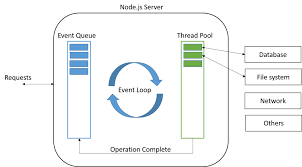
\includegraphics[scale=0.9]{figures/js-event-loop.png}
	\centering
	\caption{Βρόχος συμβάντων της \selectlanguage{english}\textit{JavaScript}\selectlanguage{greek} (Πηγή: \cite{[JS3]})}
	\label{eventloop}
\end{figure}

\subsubsection{\selectlanguage{english}Run to Completion Logic\selectlanguage{greek}}

Η πρακτική που ακολουθεί το περιβάλλον της \selectlanguage{english}JavaScript\selectlanguage{greek} είναι η πλήρης
επεξεργασία κάθε μηνύματος προτού συνεχίσει με το επόμενο. Αυτό προσφέρει
κάποιες ελκυστικές ιδιότητες κατά το σχεδιασμό της λογικής των προγραμμάτων, συμπεριλαμβανομένης της εγγύησης της εγκυρότητας των δεδομένων κατά τη διάρκεια της εκτέλεσης συναρτήσεων. Παρατηρείται δηλαδή διαφορά με το μοντέλο της \selectlanguage{english}C\selectlanguage{greek}, κατά το οποίο, όταν μία συνάρτηση ή κομμάτι κώδικα εκτελείται μέσα σε κάποιο νήμα, το σύστημα έχει τη δυνατότητα να διακόψει την εκτέλεσή τους και να μεταφέρει τον έλεγχο σε κάποιο άλλο νήμα. Βέβαια, υπάρχουν και μειονεκτήματα στην προσέγγιση αυτή, το σπουδαιότερο εκ των οποίων έχει να κάνει με το εάν ένα μήνυμα χρειαστεί σημαντικό χρονικό διάστημα για την επεξεργασία του, όλη η εφαρμογή καθίσταται ανίκανη να διαχειριστεί οποιαδήποτε αλληλεπίδραση με το χρήστη. Δεν είναι σπάνια, ακόμα και σήμερα, η εμφάνιση ειδοποίησης με τη μορφή ξεχωριστού παραθύρου από τον \selectlanguage{english}browser\selectlanguage{greek}, σύμφωνα με την οποία «η εκτέλεση κάποιου \selectlanguage{english}script\selectlanguage{greek} καθιστά την εφαρμογή μη αποκρίσιμη». Οι προγραμματιστές για να υπερκεράσουν τους περιορισμούς αυτούς προσπαθούσαν να μειώσουν όσο γίνεται το χρόνο επεξεργασίας που απαιτείτο ή, αν
αυτό δεν ήταν δυνατό, να «μοιράσουν» το φόρτο σε μικρότερα μηνύματα, τα οποία τοποθετούσαν εκ νέου στο βρόχο συμβάντων χρησιμοποιώντας ειδικά \selectlanguage{english}API calls\selectlanguage{greek}, όπως \selectlanguage{english}\textit{setTimeout()}\selectlanguage{greek} και \selectlanguage{english}\textit{setInterval()}\selectlanguage{greek}.

\subsubsection{\selectlanguage{english}Asynchronous JavaScript and XML}
\selectlanguage{greek}

Όπως έχει ήδη αναφερθεί, στο παρελθόν η \selectlanguage{english}HTML\selectlanguage{greek} αποτελούσε τη μοναδική προσέγγιση στατικών ιστοσελίδων και \selectlanguage{english}web\selectlanguage{greek} υπηρεσιών. Η εμφάνιση της \selectlanguage{english}JS\selectlanguage{greek} προσσέγισης έφερε την πραγματική επανάσταση στην ανάπτυξη εφαρμογών και διαδικτυακών προγραμμάτων. Σε αυτό συνέβαλλε κυρίως η εμφάνιση των \selectlanguage{english}AJAX\selectlanguage{greek} τεχνικών \cite{[AJAX1],[AJAX2]}, οι οποίες μετατόπισαν τον έλεγχο της ροής και της πληροφορίας από τους εξυπηρετητές στους πελάτες. Ο \selectlanguage{english}client side\selectlanguage{greek} προγραμματισμός έχει αναβαθμιστεί και πλέον είναι εφικτή η αλληλεπίδραση μεταξύ του \selectlanguage{english}backend\selectlanguage{greek} και του \selectlanguage{english}frontend\selectlanguage{greek} μιας εφαρμογής μέσω αμοιβαίων ασύγχρονων αιτημάτων. Με αυτό τον τρόπο, ο \selectlanguage{english}client\selectlanguage{greek} μπορεί να αιτηθεί δεδομένα από τον \selectlanguage{english}server\selectlanguage{greek} και, όταν αυτά είναι διαθέσιμα, να τα αναπαραστήσει ή να τα επεξεργαστεί κατάλληλα.


\subsubsection{\selectlanguage{english}Single Page Applications}
\selectlanguage{greek}
Η επόμενη καθοριστική αλλαγή ήρθε το 2002 με την είσοδο της έννοιας των εφαρμογών μονής σελίδας \textit{\textbf{--}} \selectlanguage{english}\textit{SPA}\selectlanguage{greek}. H λογική εδώ είναι ότι μια \selectlanguage{english}web\selectlanguage{greek} εφαρμογή λαμβάνει χώρα σε μία μόνο ιστοσελίδα με στόχο να παρέχει μια πιο άμεση και ομαλή
εμπειρία συγκρίσιμη με εφαρμογές επιφάνειας εργασίας (\selectlanguage{english}desktop applications\selectlanguage{greek}). Η σελίδα φορτώνεται μία μόνο φορά και στη συνέχεια τα δεδομένα φορτώνονται δυναμικά μέσω αλληλεπίδρασης \selectlanguage{english}server \textit{\textbf{--}} client\selectlanguage{greek}, ενώ ταυτόχρονα εξακολουθεί να δίνει στον χρήστη την εντύπωση οτι πλοηγείται σε διαφορετικές σελίδες, εντός της εφαρμογής \cite{[SPA1]}.

\begin{figure}[ht]
	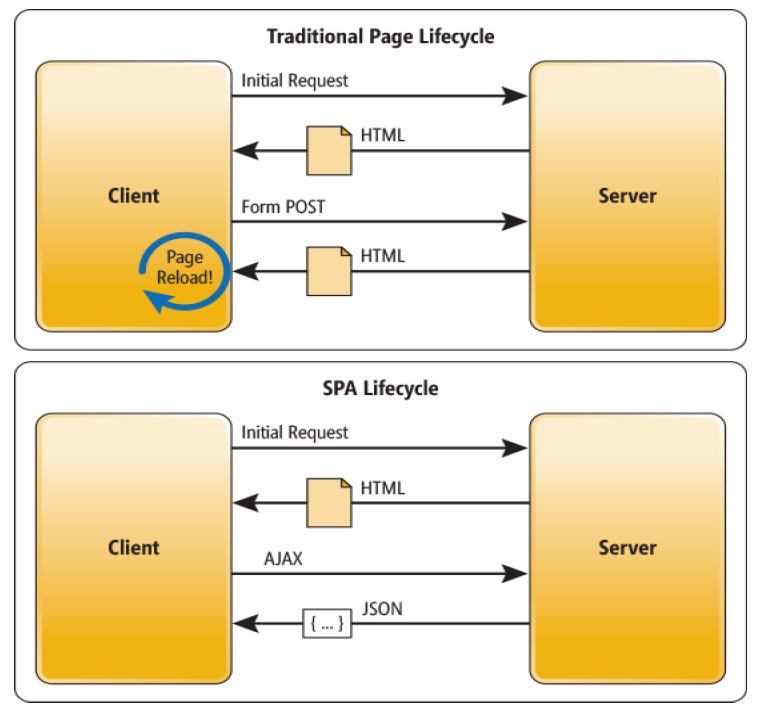
\includegraphics[scale=0.5]{figures/ajax-calls.png}
	\centering
	\caption{Διαφορές μεταξύ παραδοσιακής λογικής ιστοσελίδας και λογικής \selectlanguage{english}\textit{SPA}\selectlanguage{greek}.}
	\label{ajaxcalls}
\end{figure}

Αυτή η στροφή στον τρόπο διαχείρισης δεδομένων, κατέρριψε τα εμπόδια μεταξύ απόδοσης και πολυπλοκότητας.

\subsubsection{\selectlanguage{english}Model View Controller}
\selectlanguage{greek}
Ωστόσο, πολυπλοκότητα και η ποσότητα της λογικής που δόθηκε στον πελάτη
δημιούργησε νέα προβλήματα. Το μέγεθος του κώδικα αυξήθηκε δραματικά, και οι τεχνοτροπίες που δημιουργήθηκαν ποίκιλλαν πολύ. H λύση δόθηκε ομαδοποιώντας πρακτικές και σχεδιαστικές επιλογές σε ολοκληρωμένες τεχνοτροπίες (\selectlanguage{english}frameworks\selectlanguage{greek}) που μέχρι στιγμής υπήρχαν μόνο στους εξυπηρετητές. Η πιο γνωστή όλων
αυτών των \selectlanguage{english}JavaScript Frameworks\selectlanguage{greek} είναι η τεχνοτροπία Μοντέλου \textit{\textbf{--}} Όψης \textit{\textbf{--}} Ελεγκτή, γνωστή και ως \selectlanguage{english}\textit{MVC}\selectlanguage{greek}(βλ. Σχ. \ref{mvcmodel}), η οποία αποτελείται από τα εξής τρία μέρη:

\begin{itemize}
\item \textbf{Μοντέλα \textit{\textbf{--}} \selectlanguage{english}\textit{Models}\selectlanguage{greek}} που αναπαριστούν τις σχετικές με την εφαρμογή πληροφορίες
και δεδομένα, όπως συγκεκριμένες κλάσεις-δοχεία (\selectlanguage{english}container classes\selectlanguage{greek}) δεδομένων. Τα μοντέλα μπορούν να ενημερώνουν τυχόν παρατηρητές όταν η κατάστασή τους αλλάζει (π.χ. όταν κάποια πληροφορία που κρατούν ενημερώνεται ή διαγράφεται) \cite{[MVC1]}.
\item \textbf{Όψεις \textit{\textbf{--}} \selectlanguage{english}\textit{Views}\selectlanguage{greek}} που τυπικά θεωρούνται ως η διεπαφή του χρήστη με την εφαρμογή
(π.χ. ο κώδικας \selectlanguage{english}HTML\selectlanguage{greek} και \selectlanguage{english}CSS\selectlanguage{greek}). Πρέπει να γνωρίζουν για την ύπαρξη των
μοντέλων, έτσι ώστε να τα παρατηρούν, αλλά δεν επικοινωνούν κατευθείαν μαζί
τους.
\item \textbf{Ελεγκτές \textit{\textbf{--}} \selectlanguage{english}\textit{Controllers}\selectlanguage{greek}} που υλοποιούν τη λογική παρουσίασης (\selectlanguage{english}presentation logic\selectlanguage{greek})
της εφαρμογής. Αυτοί είναι που παίρνουν τις αποφάσεις και ο συνδετικός κρίκος μεταξύ Μοντέλων και Όψεων.
\end{itemize}

\begin{figure}[ht]
	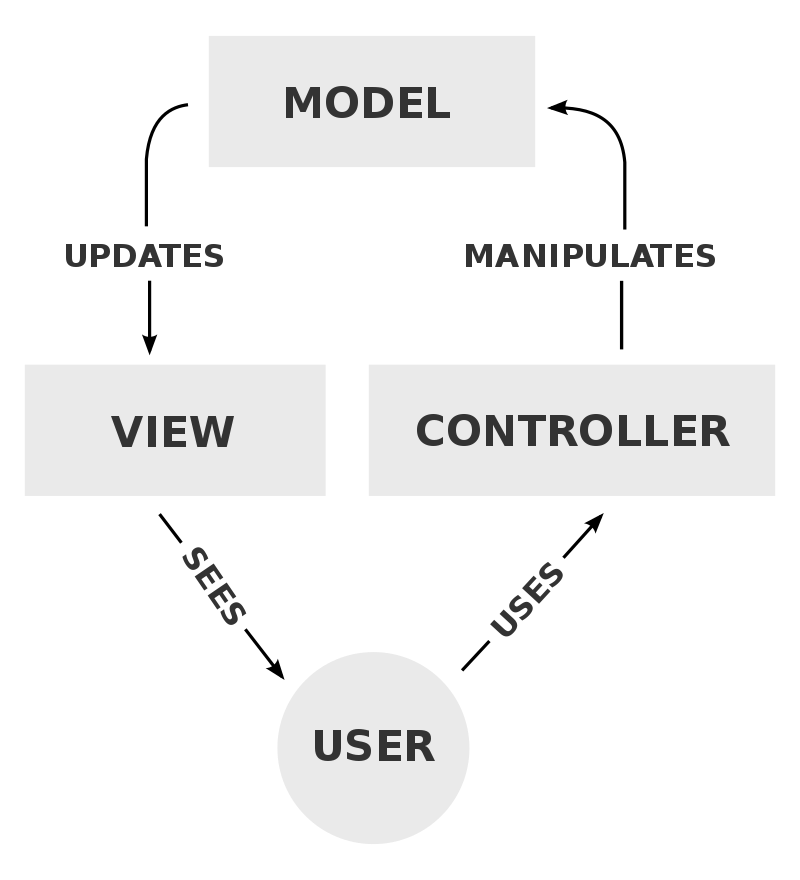
\includegraphics[scale=0.2]{figures/mvc-model.png}
	\centering
	\caption{Διάγραμμα αναπαράστασης των αλληλεπιδράσεων βάσει του μοντέλου \selectlanguage{english}\textit{MVC}\selectlanguage{greek}.}
	\label{mvcmodel}
\end{figure}


\subsection{Η Ανάγκη Μιας Νέας Τεχνολογίας - \selectlanguage{english}React Framework}
\selectlanguage{greek}
Ωστόσο, η αύξηση της πολυπλοκότητας των \selectlanguage{english}mobile applications\selectlanguage{greek} συνεπάγεται αύξηση των απαιτήσεων. Πλέον, η ανάπτυξη μιας \selectlanguage{english}native\selectlanguage{greek} εφαρμογής συνοδεύεται από πολλαπλά καθήκοντα. H υλοποίηση κώδικα που μπορεί να μεταφερθεί με ελάχιστες τροποποιήσεις μεταξύ πολλαπλών πλατφόρμων (\selectlanguage{english}cross-platform apps\selectlanguage{greek}), η ανάγκη για εφαρμογές που υποστηρίζονται και από το \selectlanguage{english}web (web apps)\selectlanguage{greek}, το συνολικό κόστος ανάπτυξης, καθώς και ο χρόνος ανάπτυξης είναι μερικοί από τους βασικότερους παράγοντες που συνέδραμαν στην αναζήτηση μιας καινοτόμου λύσης.

Έτσι, το 2011 η ομάδα προγραμματιστών του \selectlanguage{english}Facebook\selectlanguage{greek} διαμόρφωσε μια νέα τεχνολογία για την ανάπτυξη \selectlanguage{english}web\selectlanguage{greek} και \selectlanguage{english}native\selectlanguage{greek} εφαρμογών, γνωστή ως \selectlanguage{english}React\selectlanguage{greek} (\selectlanguage{english}\textit{React.js}\selectlanguage{greek} ή \selectlanguage{english}\textit{ReactJS}\selectlanguage{greek}). Τα βασικότερα χαρακτηριστικά της\selectlanguage{english} React\selectlanguage{greek} είναι:

\begin{itemize}
\item η αρχιτεκτονική διαίρεσης του κώδικα σε μικρότερα στοιχεία, τα οποία καλούνται \selectlanguage{english}components (component-based architecture)\selectlanguage{greek} \cite{[REACT1]},
\item η μονοσήμαντη ροή δεδομένων μέσω των ``\textit{ιδιοτήτων}'' (\selectlanguage{english}\textit{props}\selectlanguage{greek}) ενός στοιχείου (\selectlanguage{english}one-way data binding\selectlanguage{greek}) \cite{[REACT1]},
\item η δυνατότητα αποθήκευσης της κατάστασης ενός στοιχείου (\selectlanguage{english}stateful component\selectlanguage{greek}) και μετάδοσης της κατάστασης (\selectlanguage{english}state\selectlanguage{greek}) σε στοιχεία-παιδιά (\selectlanguage{english}child-component\selectlanguage{greek}) του στοιχείου-πατέρα (\selectlanguage{english}parent-component\selectlanguage{greek}) μέσω των \selectlanguage{english}props\selectlanguage{greek},
\item η \selectlanguage{english}JSX\selectlanguage{greek} σύνταξη \cite{[REACT3]}
\item η ανανέωση μόνο εκείνου του περιεχομένου της σελίδας που μεταββάλεται (\selectlanguage{english}virtual DOM\selectlanguage{greek}) \cite{[REACT2]} και
\item η δυνατότητα εκτέλεσης τμημάτων κώδικα σε δεδομένα χρονικά σημεία κατά τον κύκλο ζωής του στοιχείου με τη βοήθεια συγκεκριμένων \selectlanguage{english}hooks\selectlanguage{greek} (\selectlanguage{english}lifecycle methods\selectlanguage{greek}), τα βασικότερα εκ των οποίων είναι \textit{\selectlanguage{english}render(), componentDidMount(), componentWillUnmount()\selectlanguage{greek}}
\end{itemize}

H φιλοσοφία ενιαίου κώδικα σε όλες τις πλατφόρμες απέκτησε δημοτικότητα με ραγδαίους ρυθμούς. Ως αποτέλεσμα, η κοινότητα προγραμματιστών του \selectlanguage{english}Facebook\selectlanguage{greek} σηματοδότησε επισήμως το 2015 την έναρξη μιας νέας εποχής, με την ανακοίνωση της \selectlanguage{english}React Native\selectlanguage{greek}. 
 
\selectlanguage{english}
\begin{lstlisting}[language=React, caption=\selectlanguage{greek}Παράδειγμα κώδικα σε \selectlanguage{english}React\selectlanguage{greek} (Πηγή:\cite{[REACT4]})]
class Board extends React.Component {
  constructor(props) {
    super(props);
    this.state = {
      squares: Array(6).fill(null),
    };
  }

  handleClick(i) {
    const squares = this.state.squares.slice();
    squares[i] = 'X';
    this.setState({squares: squares});
  }

  renderSquare(i) {
    return (
      <Square
        value={this.state.squares[i]}
        onClick={() => this.handleClick(i)}
      />
    );
  }

  render() {
    const status = 'Next player: X';
    return (
      <div>
        <div className="status">{status}</div>
        <div className="board-row">
          {this.renderSquare(0)}
          {this.renderSquare(1)}
          {this.renderSquare(2)}
        </div>
        <div className="board-row">
          {this.renderSquare(3)}
          {this.renderSquare(4)}
          {this.renderSquare(5)}
        </div>
      </div>
    );
  }
}
\end{lstlisting}
\selectlanguage{greek}

\subsubsection{\selectlanguage{english}React Native}
\selectlanguage{greek}

Η \selectlanguage{english}React Native\selectlanguage{greek}, είναι ένα \selectlanguage{english}Framework\selectlanguage{greek} για την ανάπτυξη πραγματικών, native εφαρμογών για \selectlanguage{english}iOS\selectlanguage{greek} και \selectlanguage{english}Android\selectlanguage{greek} πλατφόρμες. Η φιλοσοφία της \selectlanguage{english}React Native\selectlanguage{greek} είναι πανονομοιότυπη με αυτή της \selectlanguage{english}React\selectlanguage{greek}, και στηρίζεται στους ίδιους κανόνες και τεχνικές που διέπουν τα πλαίσια της \selectlanguage{english}JavaScript\selectlanguage{greek}, με τη μόνη διαφορά ότι αποσκοπεί στην σχεδίαση διεπιφανειών που απευθύνονται σε πλατφόρμες κινητών συσκευών, έναντι προγραμμάτων περιήγησης. Με άλλα λόγια, αποτελεί έναν νέο τρόπο υλοποίησης εφαρμογών που δε διαφέρουν σε τίποτα από εφαρμογές γραμμένες σε \selectlanguage{english}native\selectlanguage{greek} γλώσσες προγραμματισμού (\selectlanguage{english}Swift, Java\selectlanguage{greek}). Έτσι, είναι πλέον εφικτή η ανάπτυξη εφαρμογών για πολλαπλές πλατφόρμες, με τη χρήση μιας μόνο γλώσσας, η οποία υποστηρίζεται και από τις εφαρμογές \selectlanguage{english}web\selectlanguage{greek}. Το χρονοδιάγραμμα υλοποίησης μειώνεται αισθητά, αφού η διαδικασία ανάπτυξης \selectlanguage{english}iOS\selectlanguage{greek} και \selectlanguage{english}Android\selectlanguage{greek} εφαρμογών μπορεί να γίνει τώρα παράλληλα. Εντούτοις, το κόστος ανάπτυξης της εφαρμογής δεν εξαρτάται πλέον από τη δυνατότητα ή μη υποστήριξης της εφαρμογής από περισσότερες από μια πλατφόρμες. 

Τα πλεονεκτήματα που προάγουν τη \selectlanguage{english}React Native\selectlanguage{greek} ως το δημοφιλέστερο \selectlanguage{english}cross-platform framework\selectlanguage{greek} είναι πολλά. Όπως και η \selectlanguage{english}React\selectlanguage{greek}, έτσι και η \selectlanguage{english}React Native\selectlanguage{greek} χρησιμοποιεί \selectlanguage{english}JSX\selectlanguage{greek} σύνταξη. Ωστόσο, στην υλοποίηση χρησιμοποιούνται οι μητρικές διεπαφές κάθε πλατφόρμας (\selectlanguage{english}Objective-C\selectlanguage{greek} για \selectlanguage{english}iOS\selectlanguage{greek} και \selectlanguage{english}Java\selectlanguage{greek} για \selectlanguage{english}Android\selectlanguage{greek}). Το γεγονός αυτό καθιστά τις εφαρμογές εξίσου αποδοτικές, με αυτές σε \selectlanguage{english}native\selectlanguage{greek} κώδικα. Έτσι, οι προγραμματιστές που είναι εξοικειωμένοι με την ανάπτυξη \selectlanguage{english}web\selectlanguage{greek} εφαρμογών μπορούν να εκμεταλλευτούν τη συγγένεια των δύο αυτών γλωσσών.

\paragraph{Προγραμματιστική Εμπειρία \textbf{--} \selectlanguage{english}Developer Experience\selectlanguage{greek}} 
\paragraph{}
Για προγραμματιστές με προϋπάρχουσα εμπειρία στην ανάπτυξη \selectlanguage{english}mobile\selectlanguage{greek} εφαρμογών, το περιβάλλον της \selectlanguage{english}React Native\selectlanguage{greek} είναι ιδιαίτερα φιλικό. Η ομάδα της \selectlanguage{english}React Native\selectlanguage{greek} προσφέρει στον προγραμματιστή ισχυρά προγραμματιστικά εργαλεία που διευκολύνουν τη διαδικασία ανάπτυξης μιας εφαρμογής και μειώνουν αισθητά το χρόνο προγραμματισμού. Για παράδειγμα, δεν απαιτείται \selectlanguage{english}rebuild\selectlanguage{greek} κάθε φορά που ο προγραμματιστής επιθυμεί να προβάλλει τις αλλαγές στην εφαρμογή, αλλά αρκεί μια απλή ανανέωση της σελίδας, όπως σε μια συνηθισμένη ιστοσελίδα. Αυτό εντίνει ιδιαίτερα την αμεσότητα στη διαδικασία επικοινωνίας μεταξύ κώδικα και εφαρμογής και έτσι ο προγραμματιστής μπορεί να ελέγχει τις αλλαγές του κάθε φορά. Αυτό έχει σημαντικό αντίκτυπο στην περίπτωση σχεδιασμού (\selectlanguage{english}design\selectlanguage{greek}) της εφαρμογής, όπου λεπτομερείς αλλαγές λαμβάνουν χώρα διαρκώς και η εφαρμογή μπορεί να ανανεώνεται αυτομάτως.    

Επίσης, το περιβάλλον υποστήριξης της \selectlanguage{english}React Native\selectlanguage{greek} συνοδεύεται από ολοκληρωμένη και επικαιροποιημένη βιβλιογραφία, ενώ σημαντική προσοχή δίνεται και στη διαδικασία αποσφαλμάτωσης του κώδικα μέσω επεξηγηματικών μηνυμάτων λάθους. Ο προγραμματιστής μπορεί να επωφεληθεί από τα έξυπνα εργαλεία εντοπισμού σφαλμάτων και την αναφορά σφαλμάτων που είναι ενσωματωμένα στους σύγχρονους περιηγητές όπως ο \selectlanguage{english}Chrome\selectlanguage{greek} ή ο \selectlanguage{english}Safari\selectlanguage{greek} (βλ. Σχ. \ref{debugger}). Παρομοίως, η ίδια ευελιξία χαρακτηρίζει και την επιλογή της πλατφόρμας προγραμματισμού, καθώς ο προγραμματιστής είναι ελεύθερος να επιλέξει εκείνο τον \selectlanguage{english}text editor\selectlanguage{greek} με τον οποίο διαθέτει τη μέγιστη εξοικείωση. Περιορισμοί όπως ο προγραμματισμός σε συγκεκριμένο λογισμικό για εφαρμογές \selectlanguage{english}iOS\selectlanguage{greek} ή \selectlanguage{english}Android\selectlanguage{greek}, που χαρακτηρίζουν τις \selectlanguage{english}native\selectlanguage{greek} γλώσσες προγραμματισμού (όπως αναφέρθηκε στην ενότητα 2.3.2) δεν αποτελούν εμπόδιο για την \selectlanguage{english}React Native\selectlanguage{greek}. Όλα τα παραπάνω συνεισφέρουν σε μία πρωτοποριακή και εποικοδομητική εμπειρία, που επιτρέπει την επικέτρωση στο προγραμματιστικό κομμάτι και εξασφαλίζει ταχύτητα και ευκολία.

\begin{figure}
    \centering
    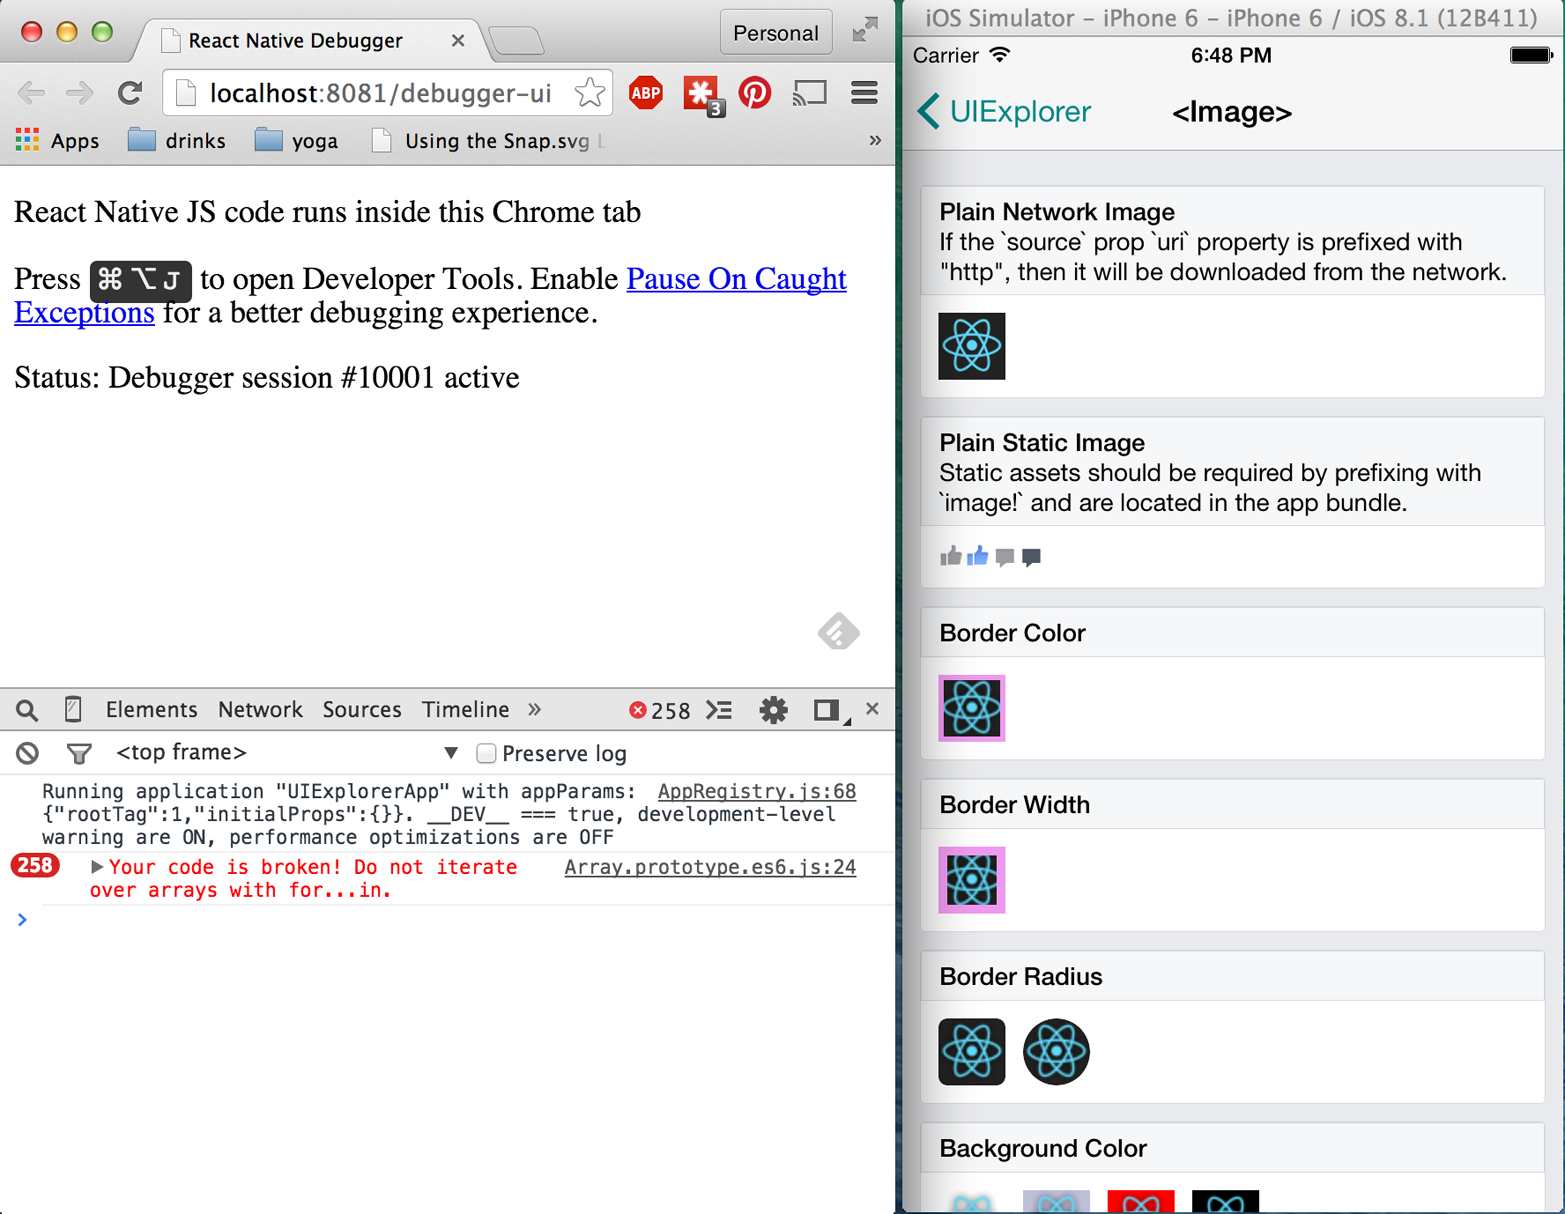
\includegraphics[scale=0.9]{figures/using-react-native-debugger.png}
    \caption{Χρήση του ενσωματωμένου αποσφαλματωτή στον περιηγητή \selectlanguage{english}Chrome\selectlanguage{greek}}
    \label{debugger}
\end{figure}

\paragraph{Επαναχρησιμότητα και Κοινή Χρήση \textbf{--} \selectlanguage{english}Code Reuse and Knowlegde Sharing\selectlanguage{greek}} 
\paragraph{}

Η εργασία στο περιβάλλον της \selectlanguage{english}React Native\selectlanguage{greek} μπορεί να ελαχιστοποιήσει δραματικά τους απαιτούμενους πόρους για την ανάπτυξη μιας \selectlanguage{english}mobile\selectlanguage{greek} εφαρμογής. Οποιοσδήποτε διαθέτει γνώση της \selectlanguage{english}React\selectlanguage{greek} μπορεί να στοχεύσει την ανάπτυξη, τόσο \selectlanguage{english}web\selectlanguage{greek} εφαρμογών, όσο και \selectlanguage{english}native\selectlanguage{greek} (\selectlanguage{english}iOS\selectlanguage{greek} και \selectlanguage{english}Android\selectlanguage{greek}) χωρίς περιορισμούς. Έτσι, παύει να υπάρχει διάκριση μεταξύ προγραμματιστών. Χρησιμοποιώντας το ίδιο σύνολο δεξιοτήτων και γνώσεων, κάθε ομάδα προγραμματιστών μπορεί να εργαστεί ταχύτερα, αμεσότερα και αποτελεσματικότερα, αφού η γνώση είναι κοινή και μπορεί να μοιραστεί ανά πάσα στιγμή.

Εκτός από την κοινή χρήση της γνώσης, μεγάλα τμήματα κώδικα μπορούν επίσης να επαχρησιμοποιηθούν. Προφανώς, ενδέχετεαι η απαίτηση περαιτέρω τροποποίησης κάποιων σημείων του κώδικα που αφορά κάθε πλατφόρμα. Παρ' όλα αυτά, η επαναχρησιμοποίηση κώδικα μεταξύ διαφόρων πλατφόρμων είναι ιδιαίτερα εύκολη και γρήγορη. Αρκούν κάποιες συνθήκες και η χρήση κάποιων διαφορετικών διεπαφών προκειμένου να καταστεί εφικτή η \selectlanguage{english}cross-platform\selectlanguage{greek} λειτουργικότητα. Για παράδειγμα, η εφαρμογή διαχείρισης διαφημίσεων του \selectlanguage{english}Facebook\selectlanguage{greek} για \selectlanguage{english}Android\selectlanguage{greek} μοιράζεται το 87\% της βάσης του κώδικα με την αντίστοιχη εφαρμογή για \selectlanguage{english}iOS\selectlanguage{greek} \cite{[RN1]}.

\paragraph{Εξοικονόμηση Πόρων \textbf{--} \selectlanguage{english}Resource Saving\selectlanguage{greek}} 
\paragraph{}

Στην εποχή αυτή της τεχνολογίας, συναντάται συχνά η απαίτηση υψηλής ποιότητας με χαμηλό κόστος. Η \selectlanguage{english}React Native\selectlanguage{greek} θεμελιώνεται σε αυτά τα δεδομένα, προσφέροντας υψηλή απόδοση με ελαχιστοποίηση των απαιτούμενων πόρων. Οι περισσότερες ηλεκτρονικές υπηρεσίες και εταιρείες σήμερα έχουν την ανάγκη να αντιπροσωπεύονται τόσο στο διαδίκτυο μέσω μιας \selectlanguage{english}web\selectlanguage{greek} εφαρμογής, όσο και στις φορητές συσκευές μέσω \selectlanguage{english}native\selectlanguage{greek} εφαρμογών. Το γεγονός ότι η χρήση φορητών συσκευών αυξάνεται με εκθετικούς ρυθμούς την τελευταίες δεκαετίες (βλ. Σχ. \ref{mobileusage}), έχει στρέψει την προσοχή στην δεύτερη κατηγορία εφαρμογών.  Όπως προαναφέρθηκε, είναι πλέον εφικτή η ανάπτυξη μιας εφαρμογής που ανταποκρίνεται σε πολλές πλατφόρμες, με ελάχιστες τροποποιήσεις. Ως αποτέλεσμα, οι ομάδες προγραμματιστών εντός μιας εταιρείας είναι μικρότερες και πιο ευέλικτες. Ακόμη, τα χρονικά πλαίσια ολοκλήρωσης μιας εφαρμογής είναι συντομότερα και δεν αυξάνονται ανάλογα με τον αριθμό πλατφόρμων υποστήριξης της εφαρμογής, όπως άλλοτε. Τέλος, είναι ευνόητο πως τα παραπάνω ευνοούν την εξοικονόμηση χρηματικών πόρων που απαιτούνται για την ανάπτυξη μιας εφαρμογής \cite{[RN2]}. Αναμφισβήτητα λοιπόν, η \selectlanguage{english}React Native\selectlanguage{greek} αποκτά μεγάλη δημοτικότητα και για αυτούς τους λόγους, γνωστές εφαρμογές όπως η \selectlanguage{english}AirBnB\selectlanguage{greek}, το \selectlanguage{english}Skype\selectlanguage{greek}, το \selectlanguage{english}Instagram\selectlanguage{greek} και το \selectlanguage{english}Facebook\selectlanguage{greek} την έχουν υιοθετήσει \cite{[RN3]}.

\begin{figure}
    \centering
    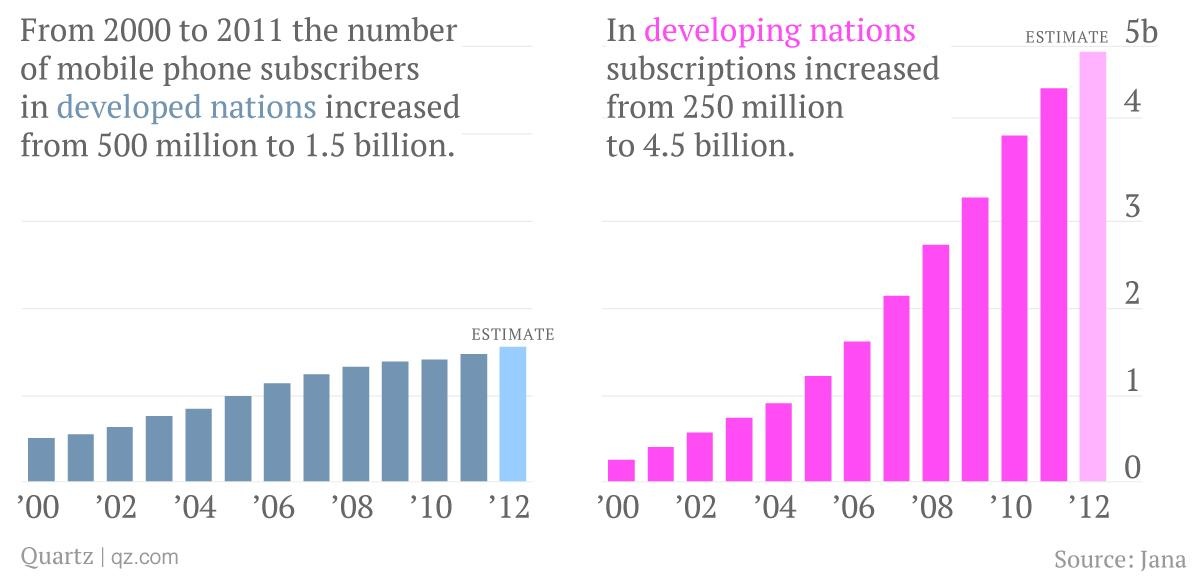
\includegraphics[scale=0.4]{figures/mobile-use.png}
    \caption{Η χρήση εφαρμογών σε κινητά αυξάνεται εκθετικά.}
    \label{mobileusage}
\end{figure}


\subsubsection{\selectlanguage{english}React Native Bridge}
\selectlanguage{greek}

Η φιλοσοφία πίσω από τον τρόπο λειτουργίας της \selectlanguage{english}React Native\selectlanguage{greek} είναι απλή. Προκειμένου να προσφέρει στον προγραμματιστή την ίδια εμπειρία με τις \selectlanguage{english}native\selectlanguage{greek} εφαρμογές, χρησιμοποιεί πανομοιότυπες διεπαφές και διεπιφάνειες με τις αντίστοιχες των \selectlanguage{english}native\selectlanguage{greek} γλωσσών. Πιο συγκεκριμένα, η \selectlanguage{english}React Native\selectlanguage{greek} απαρτίζεται από δύο τμήματα (\selectlanguage{english}realms\selectlanguage{greek}): 

\begin{itemize}
    \item το τμήμα της \selectlanguage{english}JavaScript (JavaScript Realm)\selectlanguage{greek} και
    \item το τμήμα των \selectlanguage{english}Native UIs (Native Realm)\selectlanguage{greek}
\end{itemize} 

Τα δύο τμήματα επικοινωνούν μεταξύ τους χρησιμοποιώντας μια ``\textit{γέφυρα}'' (\selectlanguage{english}bridge\selectlanguage{greek}), η οποία αποτελεί αναμφισβήτητα τον πυρήνα της αρχιτεκτονικής της \selectlanguage{english}React Native\selectlanguage{greek} (βλ. Σχ. \ref{reactnativebridge}). Η γεφύρωση αυτή των δύο παραπάνω τμηματων, αν και υλοποιημένη σε διαφορετικές τεχνολογίες, αποτελεί ουσιαστικά την βασική έννοια που προσφέρει τη δυνατότητα της αμφίδρομης και ασύγχρονης επικοινωνίας αυτών \cite{[RN4]}. Η επικοινωνία αυτή επιτυγχάνεται με τη χρήση διαλειτουργικών γλωσσών (\selectlanguage{english}interoperable languages\selectlanguage{greek}) όπως \selectlanguage{english}XML, JSON\selectlanguage{greek} κλπ. Περισσότερα για αυτές θα δούμε σε παρακάτω ενότητα (βλ. ενότητα 2.4.3).

\begin{figure}
    \centering
    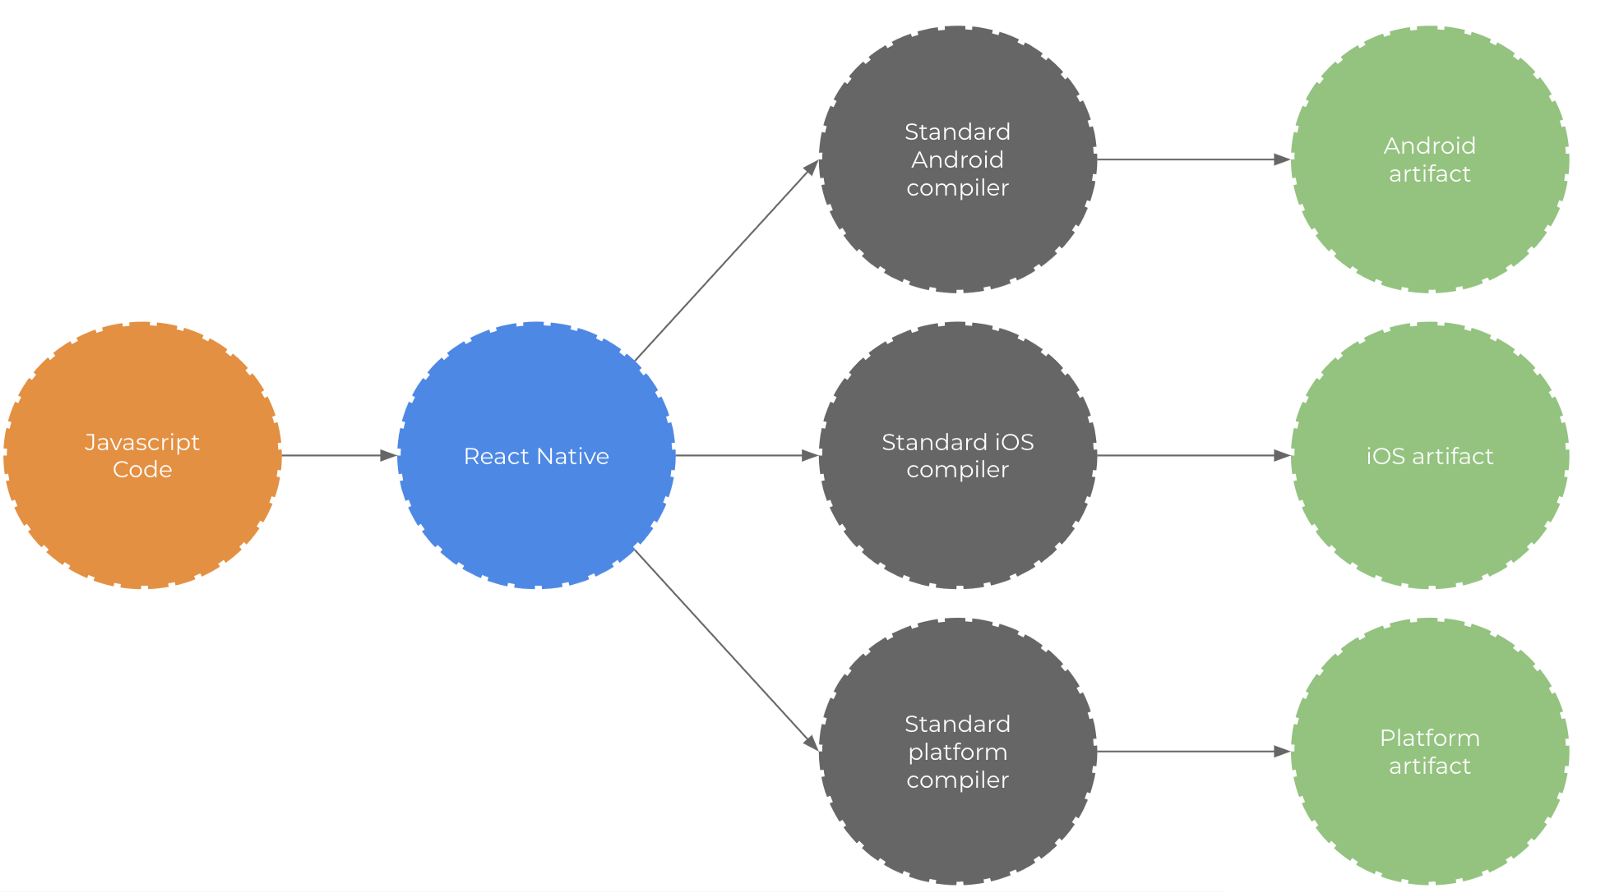
\includegraphics[scale=0.2]{figures/react-native-bridge.png}
    \caption{Η \selectlanguage{english}React Native\selectlanguage{greek} χρησιμοποιεί τα ίδια \selectlanguage{english}native UIs\selectlanguage{greek}, όπως η \selectlanguage{english}Java\selectlanguage{greek} για \selectlanguage{english}Andorid\selectlanguage{greek} και η \selectlanguage{english}Swift\selectlanguage{greek} για \selectlanguage{english}iOS\selectlanguage{greek}}
    \label{reactnativebridge}
\end{figure}

\section{Πρόσθετες Τεχνολογικές Έννοιες}
\subsection{\selectlanguage{english}Node.js}
\selectlanguage{greek}

Το \selectlanguage{english}Node.js\selectlanguage{greek} (συχνά αναφερόμενο και ως \selectlanguage{english}Node\selectlanguage{greek}) είναι ένα περιβάλλον ανοικτού κώδικα με την υποστήριξη από πολλές πλατφόρμες. Το μεγαλύτερο μέρος του είναι γραμμένο στη γλώσσα \selectlanguage{english}Javascript\selectlanguage{greek}. Το \selectlanguage{english}Node.js\selectlanguage{greek} χρησιμοποιεί τεχνικές εισόδου/εξόδου χωρίς αποκλεισμό (\selectlanguage{english}non-blocking I/O\selectlanguage{greek}), με αποτέλεσμα να παραμένει εύχρηστο και ελαφρύ όταν έρχεται αντιμέτωπο με εφαρμογές έντονου φορτίου πραγματικού χρόνου, με υψηλές απαιτήσεις μεταφοράς δεδομένων \cite{[NODE1]}. Το \selectlanguage{english}non-blocking\selectlanguage{greek} μέρος σημαίνει ότι κάποιες εντολές, όπως ανάγνωση από αρχείο, μεταβιβάζονται και εκτελούνται παράλληλα και χρησιμοποιούν μεθόδους ανάκλησης (\selectlanguage{english}callback functions\selectlanguage{greek}) για να ολοκληρώσουν το μήνυμα. Σε μία γλώσσα όπως η \selectlanguage{english}\textit{PHP}\selectlanguage{greek} για παράδειγμα, μία νέα εντολή εκτελείται μόνο αφού ολοκληρωθεί η εκτέλεση της προηγούμενης εντολής \cite{[NODE2]}. Η τεχνολογία \selectlanguage{english}Node\selectlanguage{greek} δεν είναι σχεδιασμένη να παρέχει σύνθετη υπολογιστική ισχύ σε πολύπλοκα συστήματα, δεδομένου ότι αυτό θα αναιρούσε όλα τα πλεονεκτήματά της.

Η \selectlanguage{english}Node\selectlanguage{greek} είναι μονονηματική. Συνεπώς, υπολογισμοί που καταναλώνουν πόρους μπορούν να φράξουν το νήμα και να αποτρέψουν την επεξεργασία άλλων αιτημάτων. Χρησιμοποιείται καλύτερα για τη δημιουργία γρήγορων, κλιμακούμενων δικτυακών εφαρμογών, δεδομένου ότι το μεγαλύτερο πλεονέκτημά της είναι αποτελεσμάτική διαχείριση μαζικών ταυτόχρονων συνδέσεων. Ένα άλλο τεράστιο πλεονέκτημα της \selectlanguage{english}Node.js\selectlanguage{greek} είναι η ενσωματωμένη διαχείριση πακέτων χρησιμοποιώντας το εργαλείο \selectlanguage{english}\textit{NPM}\selectlanguage{greek}. Το \selectlanguage{english}NPM\selectlanguage{greek} παρέχει στον προγραμματιστή ένα ευρύ σύνολο επαναχρησιμοποιήσιμων προγραμματιστικών εργαλείων και πακέτων, τα οποία εγκαθίστανται εύκολα και χρησιμοποιούνται κατά την ανάπτυξη εφαρμογών. Είναι ένα από τα μεγαλύτερα σύνολα βιβλιοθηκών ανοικτού κώδικα, με άριστη υποστήριξη και οργανωμένη βιβλιογραφία για κάθε πακέτο ανοιχτού κώδικα που διαθέτει \cite{[NODE3]}.

Ο τρόπος λειτουργίας του \selectlanguage{english}Node.js\selectlanguage{greek} επιδεικνύεται στο Σχ. \ref{nodesystem}. Η όλη δράση του \selectlanguage{english}Node.js\selectlanguage{greek} συγκεντρώνεται στον βρόχο συμβάντων (βλ. ενότητα 2.3.3.1). Η αποστολή ενός αιτήματος μέσα στην εφαρμογή πυροδοτεί την έναρξη ενός συμβάντος, το οποίο τοποθετείται στην ουρά συμβάντων (\selectlanguage{english}event queue\selectlanguage{greek}). Ο βρόχος συμβάντων λαμβάνει το συμβάν και το επεξεργάζεται. Σε περίπτωση που είναι αδύνατη η ολοκλήρωση ενός συμβάτνος (π.χ. ανάγνωση εικόνων), τότε η επεξεργασία του ανατίθεται σε ένα από τα νήματα εργασίας (\selectlanguage{english}worker threads\selectlanguage{greek}) από τη ``\textit{δεξαμενή νημάτων-εργαζομένων}'' (\selectlanguage{english}worker thread pool\selectlanguage{greek}). Όταν ένα νήμα εργασάις ολοκληρώση την επεξεργασία ενός συμβάτνος, επιστρέφει το μήνυμα απόκρισης χρησιμοποιώντας μια μέθοδο ανάκλησης η οποία διαβιβάστηκε σε αυτήν μέσω του συμβάντος. Το αποτέλεσμα μεταβιβάζεται στην εφαρμογή μέσω μιας μορφής \selectlanguage{english}Node\selectlanguage{greek} δεσμεύσεων \cite{[NODE2]}. 

\begin{figure}[ht]
    \centering
    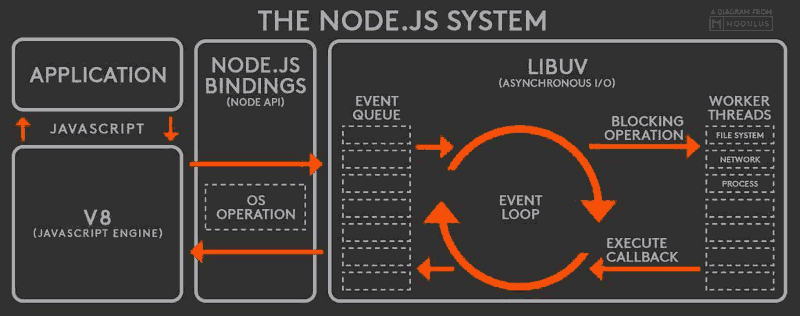
\includegraphics[scale=0.4]{figures/node-system.png}
    \caption{H αρχή λειτουργίας του συστήματος \selectlanguage{english}Node.js\selectlanguage{greek} (Πηγή: \cite{[NODE4]})}
    \label{nodesystem}
\end{figure}


Στη συνέχεια παρατίθενται τα κύρια πλεονεκτήματα της λειτουργίας ενός εξυπηρετητή \selectlanguage{english}Node.js\selectlanguage{greek}:

\begin{itemize}
    \item Ο \selectlanguage{english}Node.js server\selectlanguage{greek} μπορεί να επεξεργάζεται ασύγχρονα εισερχόμενα αιτήματα. Επομένως ο χρόνος απόκρισης είναι μικρότερος.
    \item Η \selectlanguage{english}Node.js\selectlanguage{greek} οδηγείται από συμβάντα (\selectlanguage{english}event-driven\selectlanguage{greek}) και χρησιμοποιεί \selectlanguage{english}non-blocking I/O\selectlanguage{greek}, μέσω μεθόδων επανάκλησης, του βρόχου συμβάντων και της ουράς συμβάντων. Το μοντέλο αυτό συνάδει με εκείνο των \selectlanguage{english}web servers\selectlanguage{greek}.
    \item Δεδομένου ότι βασίζεται στη \selectlanguage{english}JavaScript\selectlanguage{greek} είναι σε θέση να αξιοποιήσει το μηχανισμό \selectlanguage{english}V8 Javascript Engine\selectlanguage{greek}. Ο μηχανισμός \selectlanguage{english}V8 Javascript Engine\selectlanguage{greek} μεταγλωττίζει τον κώδικα από \selectlanguage{english}JS\selectlanguage{greek} σε κώδικα μηχανής που αποφέρει καλύτερες επιδόσεις σε σύγκριση με συνήθεις τεχνικές όπως η μετάφραση (\selectlanguage{english}interpreting\selectlanguage{greek}).
    \item Η \selectlanguage{english}Node.js\selectlanguage{greek} είναι κατάλληλη για εφαρμογές πραγματικού χρόνου που «τρέχουν» σε πολλές συσκευές. Είναι ιδανικό για γρήγορη παράδοση δεδομένων σε πολλούς αιτούντες ταυτοχρόνως.
\end{itemize}

Στο Σχ. \ref{nodevstraditional} γίνεται μια σύγκριση όσον αφορά στην επεξεργασία ενός αιτήματος μεταξύ ενός \selectlanguage{english}node server\selectlanguage{greek} και ενός συνηθισμένου \selectlanguage{english}web server\selectlanguage{greek} (όπως ο \selectlanguage{english}Apache web server\selectlanguage{greek}). Στην περίπτωση ενός \selectlanguage{english}web server\selectlanguage{greek}, σε κάθε αίτημα αντιστοιχίζεται μια νηματική διεργασία από μια δεξαμενή περιοσμένου αριθμού νημάτων. Συνεπώς, αν δεν υπάρχει διαθεσιμότητα το αίτημα τίθεται σε αναμονή έως ότου ολοκληρωθεί κάποια από τις υπόλοιπες διεργασίες. 
Η χρήση πολυνηματικών διεργασιών καταλαμβάνει αρκετό ποσοστό μνήμης στη \selectlanguage{english}RAM\selectlanguage{greek} με αποτέλεσμα την επιβράδυνση του συστήματος και άλλοτε ακόμη και τον απότομο τερματισμό αυτού. Η συμπεριφορά αυτή δεν είναι επιθυμητή. Για το λόγο αυτό, η \selectlanguage{english}Node.js\selectlanguage{greek} λειτουργεί με ένα μόνο νήμα χρησιμοποιώντας \selectlanguage{english}non-blocking I/O\selectlanguage{greek} κλήσεις, οι οποίες επιτρέπουν στο σύστημα την υποστήριξη πολλών ταυτόχρονων συνδέσεων.Για να γίνει αντιληπτό, ας υποθέσουμε ότι ο \selectlanguage{english}server\selectlanguage{greek} έχει στη διάθεσή του μια μνήμη \selectlanguage{english}RAM\selectlanguage{greek} χωρητικότητας \selectlanguage{english}8GB\selectlanguage{greek}. Επίσης, έστω ότι κάθε διεργασία καταλαμβάνει 2MB της μνήμης. Αυτό σημαίνει πως ένας παραδοσιακός web server μπορεί να επεξεργαστεί περίπου 4000 ταυτόχρονα αιτήματα. Από την άλλη πλευρά, ένας \selectlanguage{english}Node server\selectlanguage{greek} δυνητικά θα μπορούσε να επεξεργαστεί 1M ταυτόχρονα αιτήματα, χάρις την ιδιότητα επεκτασιμότητάς του \cite{[NODE1]}.

\begin{figure}[ht]
    \centering
    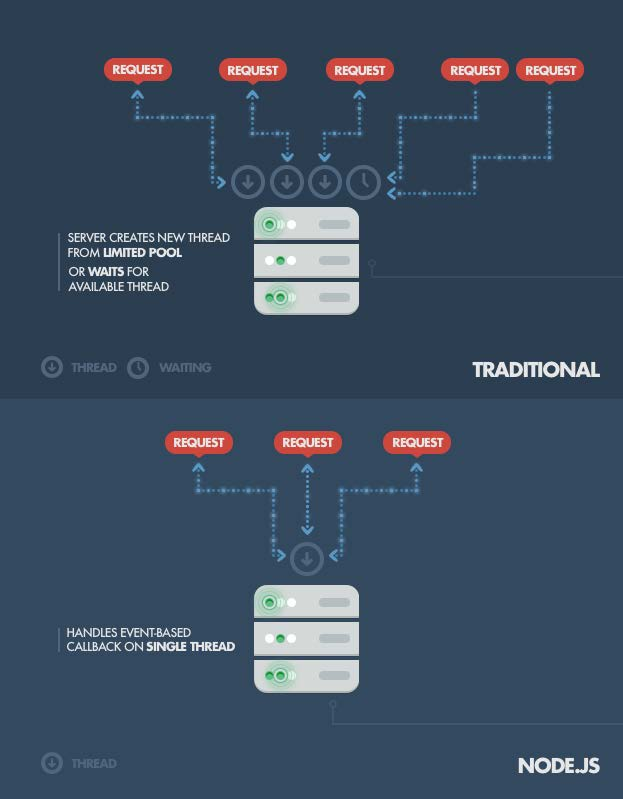
\includegraphics[scale=0.8]{figures/node-vs-tradinional-web-server.png}
    \caption{Σύγκριση ανάμεσα σε έναν \selectlanguage{english}Node.js\selectlanguage{greek} και έναν κλασσικό \selectlanguage{english}server\selectlanguage{greek}}
    \label{nodevstraditional}
\end{figure}

Εκτός από τα παραπάνω πλεονεκτήματα, ένα σημαντικό χαρακτηριστικό που καθιστά την \selectlanguage{english}Node.js\selectlanguage{greek} μία από τις κορυφαίες σύγχρονες τεχνολογίες είναι η υλοποίησή της σε \selectlanguage{english}JavaScript\selectlanguage{greek}. Το γεγονός αυτό συνεισφέρει τα μέγιστα στην ευκολία εκμάθησής της από τους προγραμματιστές που είναι ήδη εξοικειωμένοι με τη χρήση της \selectlanguage{english}JS\selectlanguage{greek}. Η προϋπόθεση της κοινής γλώσσας παίζει μείζονα ρόλο στην ανάπτυξη ολοκληρωμένων εφαρμογών (\selectlanguage{english}full stack development\selectlanguage{greek}). Έτσι, ένας προγραμματιστής έχει τη δυνατότητα να υλοποιήσει τον \selectlanguage{english}client\selectlanguage{greek} αλλά και τον \selectlanguage{english}server\selectlanguage{greek} σε μία γλώσσα (πράγμα που παλιότερα δεν ίσχυε).

\subsection{\selectlanguage{english}Representational State Transfer - REST APIs}
\selectlanguage{greek}

To \selectlanguage{english}REST\selectlanguage{greek} είναι μια μορφή αρχιτεκτονικής για τη δημιουργία δικτυακών εφαρμογών που εισήχθη το 2000 απο τον \selectlanguage{english}Roy Fielding\selectlanguage{greek} \cite{[REST2]}. Δημιουργήθηκε για να υποστηρίξει τη διαλειτουργικότητα μεταξύ όλων των υπολογιστών του διαδικτύου. Ένας \selectlanguage{english}REST Server\selectlanguage{greek} επιτρέπει την πρόσβαση πόρων μέσω κάποιου αναγνωριστικού (πχ. \selectlanguage{english}URL\selectlanguage{greek}) και ο \selectlanguage{english}REST Client\selectlanguage{greek} απλώς λαμβάνει και τροποποιεί τα δεδομένα αυτά. Οι πόροι αυτοί αναπαρίστανται με διάφορες μορφές εκ των οποίων οι πιο διαδεδομένες είναι το κείμενο, \selectlanguage{english}JSON objects, XML\selectlanguage{greek} \cite{[REST1]}. 

Η \selectlanguage{english}client\textbf{--}server\selectlanguage{greek} επικοινωνία επιτυγχάνεται μέσω αιτημάτων με ροή από τον \selectlanguage{english}client\selectlanguage{greek} στον \selectlanguage{english}server\selectlanguage{greek}. Tα αιτήματα αυτά εκκινούν από τον \selectlanguage{english}client\selectlanguage{greek} με ένα αναγνωριστικό (πχ. \selectlanguage{english}URL\selectlanguage{greek}) που αναδεικνύει τη φύση του αιτήματος, το οποίο συμβαδίζει με το endpoint που έχει δημιουργηθεί από την πλευρά του \selectlanguage{english}server\selectlanguage{greek}. Ο \selectlanguage{english}server\selectlanguage{greek} διαθέτει δρομολογητές (\selectlanguage{english}routers\selectlanguage{greek}) που αντιστοιχούν σε κάθε \selectlanguage{english}endpoint\selectlanguage{greek}. Κάθε \selectlanguage{english}router\selectlanguage{greek} έχει συγκεκριμένο ρόλο που εξυπηρετεί το αίτημα του \selectlanguage{english}client\selectlanguage{greek}. Τέλος, ο \selectlanguage{english}server\selectlanguage{greek} επιστρέφει το φορτίο (\selectlanguage{english}response payload\selectlanguage{greek}) που περιέχει τα ζητούμενα δεδομένα στον \selectlanguage{english}client\selectlanguage{greek}. Οι διεπαφές που βασίζονται σε αυτή την τεχνική ονομάζονται \selectlanguage{english}RESTful API\selectlanguage{greek} \cite{[REST3]}. Οι βασικότερες από τις διαθέσιμες μέθοδους με τις οποίες μπορεί να επιτευχθεί η παραπάνω διαδικασία είναι οι εξής:

\begin{itemize}
    \item \selectlanguage{english}\textbf{\textit{GET} --}\selectlanguage{greek}  λήψη δεδομένων από ένα \selectlanguage{english}endpoint\selectlanguage{greek}
    \item \selectlanguage{english}\textbf{\textit{POST} --}\selectlanguage{greek} αποστολή δεδομένων για αποθήκευση στο προοριζόμενο \selectlanguage{english}endpoint\selectlanguage{greek}
    \item \selectlanguage{english}\textbf{\textit{PUT} --}\selectlanguage{greek} επεξεργασία αποθηκευμένων δεδομένων στο προοριζόμενο \selectlanguage{english}endpoint\selectlanguage{greek}
     \item \selectlanguage{english}\textbf{\textit{DELETE} --}\selectlanguage{greek} διαγραφή δεδομένων από το προοριζόμενο \selectlanguage{english}endpoint\selectlanguage{greek}
\end{itemize}

Ακολουθεί επεξηγηματικός πίνακας με τις μεθόδους και την βασική αρχή λειτουργίας τους.

\begin{table}[h]
\centering
\begin{tabular}{ |m{5cm}||m{2.3cm}|m{2.3cm}|m{2.3cm}|m{2.3cm}|  }
\hline
\multicolumn{5}{|c|}{\selectlanguage{english}HTTP Methods\selectlanguage{greek}} \\
\hline 
\textit{\textbf{\selectlanguage{english}URI\selectlanguage{greek}}} & \textit{\selectlanguage{english}\textbf{GET}\selectlanguage{greek}} & \textit{\textbf{\selectlanguage{english}POST\selectlanguage{greek}}} & \textit{\textbf{\selectlanguage{english}PUT\selectlanguage{greek}}} & \textit{\textbf{\selectlanguage{english}DELETE\selectlanguage{greek}}}  \\
\hline 
\selectlanguage{english}\small{\textbf{Collection resource example}} \scriptsize{\textit{https://api.example.com/collection/}} \selectlanguage{greek}
 & \selectlanguage{english}\textit{Retrieve} the URIs of the member resources of the collection resource in the response body.\selectlanguage{greek} & \selectlanguage{english}\textit{Create} a member resource in the collection resource using the instructions in the request body. The URI of the created member resource is automatically assigned and returned in the response \textit{Location} header field.\selectlanguage{greek} & \selectlanguage{english}\textit{Replace} all the representations of the member resources of the collection resource with the representation in the request body, or create the collection resource if it does not exist.\selectlanguage{greek} & \selectlanguage{english} \textit{Delete} all the representations of the member resources of the collection resource.\selectlanguage{greek}\\
\hline
\selectlanguage{english}\small{\textbf{Member resource example}} \tiny{\textit{https://api.example.com/collection/item1}} \selectlanguage{greek}
 & \selectlanguage{english}\textit{Retrieve} a representation of the member resource in the response body.\selectlanguage{greek} & \selectlanguage{english}\textit{Create} a member resource in the member resource using the instructions in the request body. The URI of the created member resource is automatically assigned and returned in the response \textit{Location} header field.\selectlanguage{greek} & \selectlanguage{english}\textit{Replace} all the representations of the member resource, or create the member resource if it does not exist, with the representation in the request body.\selectlanguage{greek} & \selectlanguage{english} \textit{Delete} all the representations of the member resource.\selectlanguage{greek} \\

\hline  
\end{tabular}
\selectlanguage{greek}
\caption{Συνηθισμένες μέθοδοι \selectlanguage{english}HTTP\selectlanguage{greek} αιτημάτων σε \selectlanguage{english}RESTful APIs\selectlanguage{greek}}
\label{tab:parameters}
\end{table}


\clearpage

\subsection{\selectlanguage{english}JavaScript Object Notation}
\selectlanguage{greek}

Το \selectlanguage{english}JSON\selectlanguage{greek} είναι μια απλή μορφή αναπαράστασης δεδομένων ως ζεύγη ιδιοτήτων/τιμών \selectlanguage{english}(key/value)\selectlanguage{greek}. Η σύνταξή του αποτελεί υποσύνολο της γλώσσας \selectlanguage{english}JavaScript\selectlanguage{greek}, όμως κώδικας για δημιουργία και ανάλυση δομών \selectlanguage{english}JSON\selectlanguage{greek} υποστηρίζεται από μεγάλο πλήθος γλωσσών προγραμματισμού. Χρησιμοποιείται ευρέως στην ασύγχρονη επικοινωνία μεταξύ \selectlanguage{english}browser\selectlanguage{greek} και \selectlanguage{english}server\selectlanguage{greek} και τείνει να αντικαταστήσει τη γλώσσα σήμανσης \selectlanguage{english}XML\selectlanguage{greek}. Ένα αντικείμενο \selectlanguage{english}JSON\selectlanguage{greek} περικλείεται σε αγκύλες \{ \} και αποτελείται από ένα σύνολο ζευγών ιδιότητας/τιμής. Σε κάθε τέτοιο ζεύγος, η ιδιότητα είναι πάντα τύπου \selectlanguage{english}String\selectlanguage{greek}, ενώ η τιμή ανήκει σε έναν από τους τύπους δεδομένων που υποστηρίζει το \selectlanguage{english}JSON\selectlanguage{greek}. Οι υποστηριζόμενοι τύποι δεδομένων είναι οι αριθμοί (δε γίνεται διάκριση μεταξύ ακεραίων και δεκαδικών), \selectlanguage{english}Strings\selectlanguage{greek}, \selectlanguage{english}Boolean\selectlanguage{greek}, \selectlanguage{english}Arrays\selectlanguage{greek}, \selectlanguage{english}Objects\selectlanguage{greek} (συλλογή από ζεύγη ιδιοτήτων/τιμών) και το \selectlanguage{english}null\selectlanguage{greek}, που αντιπροσωπεύει την κενή τιμή.

\selectlanguage{english}
\begin{lstlisting}[language=JSON, caption=\selectlanguage{greek}Αναπαράσταση δεδομένων σε μορφή \selectlanguage{english}JSON\selectlanguage{greek}]
{
  "firstName": "John",
  "lastName": "Smith",
  "isAlive": true,
  "age": 27,
  "address": {
    "streetAddress": "21 2nd Street",
    "city": "New York",
    "state": "NY",
    "postalCode": "10021-3100"
  },
  "phoneNumbers": [
    {
      "type": "home",
      "number": "212 555-1234"
    },
    {
      "type": "office",
      "number": "646 555-4567"
    },
    {
      "type": "mobile",
      "number": "123 456-7890"
    }
  ],
  "children": [],
  "spouse": null
}
\end{lstlisting}
\selectlanguage{greek}

\clearpage

\subsection{Βάση Δεδομένων \selectlanguage{english}MongoDB}
\selectlanguage{greek}

Η \selectlanguage{english}MongoDB\selectlanguage{greek} είναι μια μη-σχετικιστική (\selectlanguage{english}non-relational\selectlanguage{greek}) βάση δεδομένων με υποστήριξη σε πολλές πλατφόρμες, που χρησιμοποιεί έγγραφα για την καταγραφή δεδομένων (\selectlanguage{english}document-oriented\selectlanguage{greek}). Η αποθήκευση των δεδομένων γίνεται με ομαδοποίηση σε ``\textit{συλλογές}'' (\selectlanguage{english}collections\selectlanguage{greek}). Κάθε \selectlanguage{english}collection\selectlanguage{greek} ακολουθεί συγκεκριμένη μοντελοποίηση ως προς την διαρρύθμιση των δεδομένων. Το μοντέλο αυτό (\selectlanguage{english}schema\selectlanguage{greek}) είναι υπεύθυνο για τον προσδιορισμό της δομής των στοιχείων που θα αποθηκευτούν σε κάθε \selectlanguage{english}collection\selectlanguage{greek} της βάσης και έχει μορφή \selectlanguage{english}JSON\selectlanguage{greek} κειμένου. 

Τα κυριότερα χαρακτηριστικά της \selectlanguage{english}MongoDB\selectlanguage{greek} συνοψίζονται παρακάτω:

\begin{itemize}
    \item \selectlanguage{english}\textbf{Ad Hoc queries --}\selectlanguage{greek} Η \selectlanguage{english}MongoDB\selectlanguage{greek} υποστηρίζει διάφορες μορφές αναζήτησης δεδομένων εντός της βάσης \cite{[MONGO1]}, όπως αναζήτηση με κριτήριο ένα συγκεκριμένο πεδίο (\selectlanguage{english}field search\selectlanguage{greek}), με τήρηση συνθήκης (\selectlanguage{english}range search\selectlanguage{greek}), ή με βάση μια σειρά χαρακτήρων που αποτελούν ένα μοτίβο αναζήτησης (\selectlanguage{english}regular expression search\selectlanguage{greek}). Το αποτέλεσμα που επιστρέφεται από μια τέτοια αναζήτηση μπορεί να είναι ένα συγκεκριμένο πεδίο ενός εγγράφου, να περιέχει μια ομάδα πεδίων ή να αποτελείται από ένα σύνολο εγγράφων δεδομένου μεγέθους.
    \item \selectlanguage{english}\textbf{Replication --}\selectlanguage{greek} Η \selectlanguage{english}MongoDB\selectlanguage{greek} παρέχει υψηλή διαθεσιμότητα με ομάδες αναπαραγωγής (\selectlanguage{english}replica sets\selectlanguage{greek}) \cite{[MONGO2]}. Ένα \selectlanguage{english}replica set\selectlanguage{greek} αποτελείται από δύο ή περισσότερα αντίγραφα των δεδομένων. Κάθε μέλος ομάδας αναπαραγωγής μπορεί να ενεργεί στο ρόλο πρωτογενούς ή δευτερογενούς αντιγράφου ανά πάσα στιγμή. Όλες οι εγγραφές και οι αναγνώσεις γίνονται στο κύριο αντίγραφο από προεπιλογή. Τα δευτερεύοντα αντίγραφα διατηρούν ένα αντίγραφο των δεδομένων του πρωτογενούς χρησιμοποιώντας την ενσωματωμένη αναπαραγωγή. Όταν ένα πρωτότυπο αντίγραφο αποτύχει, το σύνολο αντιτύπων διεξάγει αυτόματα μια εκλογική διαδικασία για να προσδιορίσει ποιο δευτερεύον πρέπει να γίνει το κύριο. Τα δευτερεύοντα τμήματα μπορούν προαιρετικά να προβάλλουν λειτουργίες ανάγνωσης (βλ. Σχ. \ref{replicaset}).
    
    \begin{figure}[h]
        \centering
        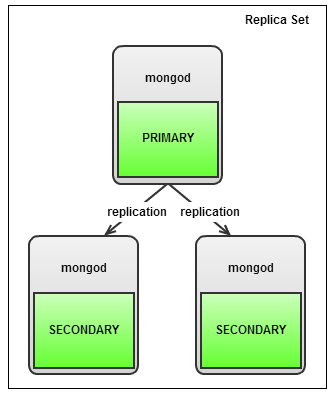
\includegraphics[scale=0.4]{figures/repset.png}
        \caption{Δομή ομάδας αντιγραφής}
        \label{replicaset}
    \end{figure}
    
    \item \selectlanguage{english}\textbf{Indexing --}\selectlanguage{greek} Τα πεδία σε μια \selectlanguage{english}MongoDB\selectlanguage{greek} βάση δεδομένων ακολουθούν μηδενική, πρωτοβάθμια ή δευτεροβάθμια δεικτοδότηση. Ο δείτκης αυτός αφορά την μοναδικότητα ή μη ενός πεδίου στη βάση.
    \item \selectlanguage{english}\textbf{Load balancing --}\selectlanguage{greek}  Η \selectlanguage{english}MongoDB\selectlanguage{greek} κλιμακώνεται οριζοντίως με τη χρήση της ιδιότητας τεμαχιοποίησης (\selectlanguage{english}sharding\selectlanguage{greek}). Ο χρήστης επιλέγει ένα ``\textit{κλειδί κοπής}'' (\selectlanguage{english}shard key\selectlanguage{greek}) το οποίο καθορίζει τον τρόπο κατανομής των δεδομένων μιας συλλογής. Τα δεδομένα χωρίζονται σε εύρη τιμών (με βάση το κλειδί αυτό) και κατανέμονται σε πολλαπλά \selectlanguage{english}shards\selectlanguage{greek} (ένα \selectlanguage{english}shard\selectlanguage{greek} είναι to κύριο έγγραφο και έχει ένα ή περισσότερα αντίγραφα). Εναλλακτικά, το κλειδί \selectlanguage{english}shard\selectlanguage{greek} μπορεί να κρυπτογραφηθεί μέσω \selectlanguage{english}hashing\selectlanguage{greek} για να χαρτογραφηθεί σε ένα \selectlanguage{english}shard\selectlanguage{greek} \textbf{--} επιτρέποντας μια ομοιόμορφη κατανομή δεδομένων. Η \selectlanguage{english}MongoDB\selectlanguage{greek} μπορεί να τρέξει σε πολλούς διακομιστές, εξισορροπώντας το φορτίο ή να αντιγράψει τα δεδομένα για να διατηρήσει το σύστημα σε λειτουργία και σε περίπτωση αποτυχίας υλικού \cite{[MONGO3]}.
     \item \selectlanguage{english}\textbf{File Storage --}\selectlanguage{greek}  Η \selectlanguage{english}MongoDB\selectlanguage{greek} μπορεί να χρησιμοποιηθεί ως σύστημα αρχείων, το οποίο ονομάζεται \selectlanguage{english}GridFS\selectlanguage{greek} \cite{[MONGO4]}, με δυνατότητες εξισορρόπησης φορτίου και αναπαραγωγής δεδομένων σε πολλαπλές μηχανές αποθήκευσης αρχείων. Το σύστημα \selectlanguage{english}GridFS\selectlanguage{greek} διαιρεί ένα αρχείο σε τμήματα, ή κομμάτια, και αποθηκεύει κάθε ένα από αυτά τα κομμάτια ως ξεχωριστό έγγραφο \cite{[MONGO5]}.
     \item \selectlanguage{english}\textbf{Aggregation --}\selectlanguage{greek}  Η \selectlanguage{english}MongoDB\selectlanguage{greek} διαθέτει τρεις μεθόδους συνάθροισης: του αγωγού συσσωμάτωσης (\selectlanguage{english}aggregation pipeline\selectlanguage{greek}), της άθροισης μέσω χαρτογράφησης (\selectlanguage{english}map-reduce function\selectlanguage{greek}) και τις μονού σκοπού μεθόδους συνάθροισης (\selectlanguage{english}single-purpose aggregation methods\selectlanguage{greek}) \cite{[MONGO6],[MONGO7]}.
\end{itemize}

Συμπερασματικά, η \selectlanguage{english}MongoDB\selectlanguage{greek} είναι σχεδιασμένη για να απλοποιήσει τη διαδικασία αποθήκευσης και αναζήτης δεδομένων. Δεν έχει συνθετες εντολές, αντιθέτως κάθε διαδικασία αναζήτησης είναι σαφής και σύντομη. Ο χρήστης παρέχει τις προϋποθέσεις ή τη συνθήκη που επιθυμεί και η \selectlanguage{english}MongoDB\selectlanguage{greek} επιστρέφει το αποτέλεσμα από τη βάση. Στην περίπτωση εύρεσης ενός εγγράφου κάνει συγκεκριμένη αναζήτηση, ενώ στην περίπτωση εύρεσης ενός πλήθους εγγράφων κάνει ομαδική αναζήτηση με σελιδοποίηση (\selectlanguage{english}pagination\selectlanguage{greek}). Η \selectlanguage{english}MongoDB\selectlanguage{greek}  είναι ευέλικτη και εύκολη στη χρήση, χάρις στην \selectlanguage{english}JSON\selectlanguage{greek} μορφοποίηση των δεδομένων, έναντι της χρήσης πικάνων (πχ. όπως στην \selectlanguage{english}SQL\selectlanguage{greek}). 


\subsection{Tαυτοποίηση Χρηστών (\selectlanguage{english}Open Authentication)}
\selectlanguage{greek}

Η ύπαρξη πολλών χρηστών σε μια εφαρμογή γεννά δύο βασικά προβλήματα. Το πρώτο συνίσταται από την ανάγκη διαχωρισμού των χρηστών μεταξύ τους, ενώ το δεύτερο έχει να κάνει με την παροχή προσωποποιημένων υπηρεσιών σε κάθε χρήστη. Σε αυτή την ενότητα γίνεται λόγος για τον τρόπο με τον οποίο επιλύονται τα παραπάνω προβλήματα. 

Οι εφαρμογές που δίνουν στους χρήστες τη δυνατότητα δημιουργίας προσωπικού λογαριασμού διαθέτουν ένα σύστημα επιβεβαίωσης και πρόσβασης εντός των υπηρεσιών τους. Το σύστημα αυτό ακολουθεί ένα πρωτόκολλο ταυτοποίησης γνωστό ως\selectlanguage{english} OAuth\selectlanguage{greek}.

\subsubsection{\selectlanguage{english}OAuth}
\selectlanguage{greek}

Το \selectlanguage{english}\textit{OAuth}\selectlanguage{greek} είναι ένα ανοιχτό πρότυπο το οποίο αναλαμβάνει την διαχείριση πρόσβασης στις υπηρεσίες μιας εφαρμογής από τους χρήστες της. Ο μηχανισμός αυτός χρησιμοποιείται σε όλες τις σημερινές εφαρμογές, όπως \selectlanguage{english}\textit{facebook, Microsoft, Google, Twitter, Amazon}\selectlanguage{greek} κλπ. Γενικά, το \selectlanguage{english}OAuth\selectlanguage{greek} παρέχει στους πελάτες μια ``\textit{ασφαλή εξουσιοδοτημένη πρόσβαση}'' σε πόρους ενός \selectlanguage{english}server\selectlanguage{greek} εξ' ονόματος του ιδιοκτήτη των πόρων αυτών. Καθορίζει μια διαδικασία εξουσιοδότησης πρόσβασης στους πόρους αυτούς σε τρίτους, χωρίς να μοιράζονται τα διαπιστευτήρια τους. Σχεδιασμένο ειδικά για να λειτουργεί με το πρωτόκολλο \selectlanguage{english}HTTP\selectlanguage{greek}, το \selectlanguage{english}OAuth\selectlanguage{greek} ουσιαστικά επιτρέπει την έκδοση πιστοποιητικών πρόσβασης σε πελάτες τρίτων μέσω ενός \selectlanguage{english}server\selectlanguage{greek} εξουσιοδότησης, με την έγκριση του ιδιοκτήτη πόρων. Το τρίτο μέρος χρησιμοποιεί το διακριτικό πρόσβασης για πρόσβαση στους προστατευόμενους πόρους που φιλοξενεί ο \selectlanguage{english}server\selectlanguage{greek} πόρων.

\subsubsection{\selectlanguage{english}Access Token}
\selectlanguage{greek}

Το σύμβολο πιστοποίησης (\selectlanguage{english}Access Token\selectlanguage{greek}) είναι ένα είδος πιστοποιητικού, το οποίο ένας πελάτης μπορεί να χρησιμοποιήσει για να αποκτήσει πρόσβαση σε προστατευμένους πόρους. Συγκεκριμένα είναι μία συμβολοσειρά χωρίς κάποια σημασία σε κανέναν εκτός από τον \selectlanguage{english}server\selectlanguage{greek}. Πέραν του ότι είναι μικρά σε μέγεθος και δεν προσθέτουν καθυστερήσεις, εμποδίζουν να χρησιμοποιούνται τα διαπεστευτήρια του ιδιοκτήτη (\selectlanguage{english}username, email, password\selectlanguage{greek}) συνεχώς και έτσι αν πέσει σε λάθος χέρια δεν τα αποκτά ο κακόβουλος χρήστης. Επιπλέον έχουν περιορισμένη πρόσβαση και συνήθως έχουν ημερομηνία λήξης, ώστε όταν αυτή παρέλθει, το σύμβολο αυτό παύει να ισχύει και δεν μπορεί να ξαναχρησιμοποιηθεί. Τότε, πρέπει να γίνει αίτηση για ανανέωση της ημερομηνίας (\selectlanguage{english}Refresh Token\selectlanguage{greek}).

Η διαδικασία ταυτοποίησης και έκδοσης \selectlanguage{english}access token\selectlanguage{greek} διακρίνεται σε τρία στάδια. Όταν ο χρήστης εισέρχεται για πρώτη φορά στην εφαρμογή, καλείται να δημιουργήσει λογαριασμό. Με αυτό τον τρόπο, ο χρήστης αποκτά πρόσβαση στους προστατευόμενους πόρους, καθώς επίσης και στις εξατομικευμένες εμπειρίες της εφαρμογής. Η είσοδος του χρήστη στην εφαρμογή γίνεται μέσω της συμπλήρωσης μιας φόρμας εγγραφής (\selectlanguage{english}register/signup form\selectlanguage{greek}). Η διαδικασία αυτή αποτελεί το πρώτο στάδιο. Αφού ο χρήστης χορηγήσει άδεια διαχείρισης των διαπιστευτηρίων του κάνοντας \selectlanguage{english}register\selectlanguage{greek} στην εφαρμογή, τότε μεταφέρεται αυτόματα εντός των υπηρεσιών της εφαρμογής. Κατά τη διάρεκεια της μετάβασης, ο \selectlanguage{english}server\selectlanguage{greek} είναι υπεύθυνος για την αποθήκευση των διαπιστευτηρίων του χρήστη και την ανταλλαγή (\selectlanguage{english}handshake\selectlanguage{greek}) τους με ένα μοναδικό \selectlanguage{english}access token\selectlanguage{greek} που αντιστοιχεί σε αυτόν τον χρήστη που μόλις πραγματοποίησε είσοδο στην εφαρμογή. Με άλλα λόγια, το \selectlanguage{english}access token\selectlanguage{greek} συμβολίζει το ``\textit{κλειδί}'' με το οποίο ο χρήστης ``\textit{ανοίγει}'' την εφαρμογή. Η ανταλλαγή αυτή αποτελεί το δεύτερο στάδιο.

Η διαδικασία αυτή είναι μονόδρομη, καθώς το πρώτο σταδιο αποτελεί απαραίτητη και αναγκαία συνθήκη για τη μετάβαση στο δεύτερο στάδιο. Ο χρήστης δεν μπορεί να παρακάμψει το πρώτο στάδιο καθώς η έκδοση \selectlanguage{english}access token\selectlanguage{greek} είναι υποχρεωτική για όλους τους χρήστες που επιθυμούν να καταναλώσουν τις υπηρεσίες τις εφαρμογής. Ωστόσο, μετά την έκδοση \selectlanguage{english}access token\selectlanguage{greek} ο χρήστης δεν χρειάζεται να επαναλάβει τη διαδικασία ταυτοποίησης. Εφόσον δεν πραγματοποιήσει έξοδο (\selectlanguage{english}logout\selectlanguage{greek}) από την εφαρμογή, έχει την δυνατότητα να «κλείσει» και να «ανοίξει» την εφαρμογή χωρίς την απαίτηση των διαπιστευτηρίων του. Το κλειδί αποθηκεύεται στη μνήμη της συσκευής για μελλοντική χρήση. Αυτό είναι και το νόημα της όλης διαδικασίας. Σε αυτή την περίπτωση, ο χρήστης κάνει είσοδο στην εφαρμογή παρακάμπτοντας το πρώτο στάδιο ταυτοποίησης, το οποίο γίνεται αυτόματα χάρις στο αποθηκευμένο κλειδί που είναι διαθέσιμο ασύγχρονα στην εφαρμογή. 

Για όσο διάστημα ο χρήστης έχει στη διάθεσή του κλειδί, μπορεί να είσερχεται στην εφαρμογή ή να εξέρχεται από αυτή κατ' επανάληψη. Αυτό οφείλεται στο γεγονός ότι ο χρήστης εξακολουθεί να είναι συνδεδεμένος. Ωστόσο, εάν για κάποιο λόγο ο χρήστης αποφασίσει να αποσυνδεθεί από την εφαρμογή κάνοντας \selectlanguage{english}logout\selectlanguage{greek}, τότε το \selectlanguage{english}access token\selectlanguage{greek} αφαιρείται και καταστρέφεται και ο χρήστης επαναφέρεται αυτόματα στην σελίδα εισόδου της εφαρμογής. Αυτή η διαδικασία αποτελεί το τρίτο και τελευταίο στάδιο, με το οποίο ολοκληρώνεται ο κύκλος ταυτοποίησης ενός χρήστη. Προκειμένου να αποκτηθεί εκ νέου πρόσβαση, πρέπει να επναληφθούν τα πρώτα δύο στάδια από την αρχή. Η μόνη διαφορά στην όλη διαδικασία είναι πως πλέον ο χρήστης είναι καταχωρημένος στη βάση της εφαρμογής και, επομένως δεν χρειάζεται να κάνει εκ νέου εγγραφή. Αρκεί να παρέχει τα διαπιστευτήριά του στην φόρμα εισόδου (\tl{login/signin form}) και στην περίπτωση επιτυχούς διασταύρωσης των στοιχείων, να συνδεθεί στο λογαριασμό του και να μεταφερθεί εντός της εφαρμογής.

\begin{figure}[h]
    \centering
    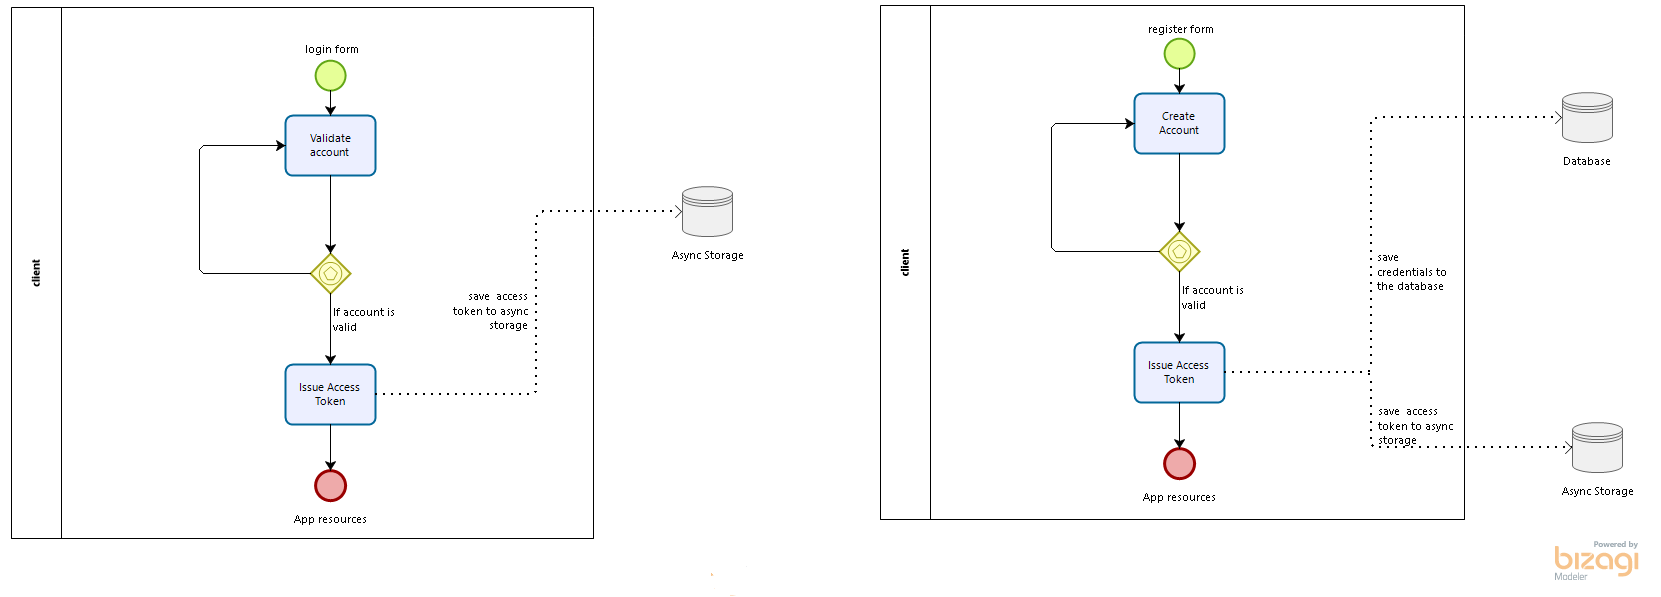
\includegraphics[scale=0.4]{figures/access-token.png}
    \caption{Διαδικασία έκδοσης \selectlanguage{english}access token\selectlanguage{greek}}
    \label{accesstoken}
\end{figure}


\subsubsection{\selectlanguage{english}JSON Web Token}
\selectlanguage{greek}

Το \selectlanguage{english}JWT\selectlanguage{greek} είναι μια μορφή \selectlanguage{english}access token\selectlanguage{greek} το οποίο εκδίδεται στην πλευρά του \selectlanguage{english}server\selectlanguage{greek} κατά την ταυτοποίηση ενός χρήστη. Κατά την επιτυχή είσοδο του χρήστη στην εφαρμογή, το \tl{JWT} αποθηκεύεται τοπικά στη μνήμη της συσκευής. Κάθε φορά που ο χρήστης θέλει να αποκτήσει πρόσβαση σε προστατευόμενους πόρους εντός της εφαρμογής, ανταλλάσσει το \selectlanguage{english}JWT\selectlanguage{greek} με τον προστατευόμενο πόρο μέσω μιας χειραψίας (\selectlanguage{english}handshake\selectlanguage{greek}). Η χειραψία είναι στην ουσία ένα αίτημα το οποίο αποστέλλεται στον \selectlanguage{english}server\selectlanguage{greek} και περιέχει, μεταξύ άλλων, και μια επικεφαλίδα εξουσιοδότησης (\selectlanguage{english}authorization header\selectlanguage{greek}). Το περιεχόμενο της επικεφαλίδας μοιάζει με το ακόλουθο:

\selectlanguage{english}
\begin{lstlisting}
Authorization: Bearer eyJhbGci...<snip>...yu5CSpyHI
\end{lstlisting}
\selectlanguage{greek}

Αυτός είναι ένας μηχανισμός ελέγχου ταυτότητας χωρίς κατάσταση, αφόυ η κατάσταση του χρήστη δεν αποθηκεύεται ποτέ στη μνήμη του \selectlanguage{english}server\selectlanguage{greek}. Οι προστατευμένες διαδρομές (\selectlanguage{english}routes\selectlanguage{greek}) του \selectlanguage{english}server\selectlanguage{greek} θα ελέγχουν την ύπαρξη έγκυρου \selectlanguage{english}JWT\selectlanguage{greek} στην επικεφαλίδα εξουσιοδότησης και, αν υπάρχει, ο χρήστης θα έχει πρόσβαση στους προστατευμένους πόρους. Καθώς τα \selectlanguage{english}JWTs\selectlanguage{greek} είναι αυτοτελή, υπάρχουν όλες οι απαραίτητες πληροφορίες, μειώνοντας την ανάγκη συχνών προσπελάσεων της βάσης δεδομένων \cite{[JWT1]}.

Τα βασικά πεδία που διαθέτει ένα \selectlanguage{english}JSON Web Token\selectlanguage{greek} φαίνονται στον κάτωθι πίνακα:


\begin{table}[h]
\centering
\begin{tabular}{ |m{2cm}|m{2cm}|m{8cm}|  }
\hline
\multicolumn{3}{|c|}{\selectlanguage{english}Standard JWT Fields\selectlanguage{greek}} \\
\hline 
\textit{\textbf{\selectlanguage{english}code\selectlanguage{greek}}} & \textit{\selectlanguage{english}\textbf{name}\selectlanguage{greek}} & \textit{\textbf{\selectlanguage{english}description\selectlanguage{greek}}}  \\
\hline 
\selectlanguage{english}\textit{iss} \selectlanguage{greek}
 & \selectlanguage{english}Issuer\selectlanguage{greek} & \selectlanguage{english}Identifies principal that issued the JWT.\\
\hline
\selectlanguage{english}\textit{sub} \selectlanguage{greek}
 & \selectlanguage{english}Subject\selectlanguage{greek} & \selectlanguage{english}Identifies the subject of the JWT.\\
\hline
\selectlanguage{english}\textit{aud} \selectlanguage{greek}
 & \selectlanguage{english}Audience\selectlanguage{greek} & \selectlanguage{english}Identifies the recipients that the JWT is intended for. Each principal intended to process the JWT \textbf{must} identify itself with a value in the audience claim. If the principal processing the claim does not identify itself with a value in the \textit{aud} claim when this claim is present, then the JWT \textbf{must} be rejected.\\
\hline
\selectlanguage{english}\textit{exp} \selectlanguage{greek}
 & \selectlanguage{english}Expiration Time\selectlanguage{greek} & \selectlanguage{english}Identifies the expiration time on and after which the JWT \textbf{must not} be accepted for processing. The value must be a \textit{NumericDate}: either an integer or decimal, representing seconds past \textit{1970-01-01 00:00:00Z.}\\
\hline
\selectlanguage{english}\textit{nbf} \selectlanguage{greek}
 & \selectlanguage{english}Not Before\selectlanguage{greek} & \selectlanguage{english}Identifies the time on which the JWT will start to be accepted for processing. The value must be a \textit{NumericDate}.\\
\hline
\selectlanguage{english}\textit{iat} \selectlanguage{greek}
 & \selectlanguage{english}Issued At\selectlanguage{greek} & \selectlanguage{english}Identifies the time at which the JWT was issued. The value must be a \textit{NumericDate}.\\
\hline
\selectlanguage{english}\textit{jti} \selectlanguage{greek}
 & \selectlanguage{english}JWT ID\selectlanguage{greek} & \selectlanguage{english}Case sensitive unique identifier of the token even among different issuers.\\
\hline
\end{tabular}
\selectlanguage{greek}
\caption{Δικαιώματα που μπορούν να αποδωθούν σε ένα \selectlanguage{english}JSON Web Token\selectlanguage{greek}}
\label{tab:parameters}
\end{table}



\subsubsection{\selectlanguage{english}Passport.js - Passport Strategies}
\selectlanguage{greek}

Για την ταυτοποίηση των χρηστών στην εφαρμογή χρησιμοποιήθηκε το λογισμικό \selectlanguage{english}Passport.js\selectlanguage{greek}. Το \selectlanguage{english}Passport\selectlanguage{greek} είναι ένα ενδιάμεσο λογισμικό το οποίο υλοποιείται σε \selectlanguage{english}JS\selectlanguage{greek} και υποστηρίζεται από τη \selectlanguage{english}Node.js\selectlanguage{greek}. Eίναι υπεύθυνο για την διαχείριση των χρηστών και την προστασία των πόρων της εφαρμογής. Συγκεκριμένα, πραγματοποιεί αναζήτηση στη βάση ενός χρήστη που επιχειρεί είσοδο στην εφαρμογή και σε περίπτωση επιτυχούς εύρεσης, εκδίδει \selectlanguage{english}token\selectlanguage{greek}.

Η προστασία των πόρων της εφαρμογής γίνεται με την υλοποίηση στατηγικών πακέτων (\selectlanguage{english}Strategies\selectlanguage{greek}) που διατίθενται από κατασκευής εντός της τεχνολογίας του \selectlanguage{english}Passport\selectlanguage{greek}. Στην εφαρμογή έγινε χρήση δύο εξ' αυτών:

\begin{itemize}
    \item \selectlanguage{english}\textbf{JWT Strategy}\selectlanguage{greek}
    \item \selectlanguage{english}\textbf{Local Strategy}\selectlanguage{greek}
\end{itemize}

Η \selectlanguage{english}JWT Strategy\selectlanguage{greek} αναλαμβάνει την προστασία των πόρων της εφαρμογής από μη εγγεγραμμένους χρήστες. Αυτό επιτυγχάνεται με τον έλεγχο κάθε φορά που γίνεται αίτημα της επικεφαλίδας εξουσιοδότητης. Εάν αυτή φέρει κάποιο \selectlanguage{english}token\selectlanguage{greek} τότε επιτρέπεται η πρόσβαση στους ζητούμενους πόρους. Αυτή η διαδικασία αποτελεί το αντίστροφο της χειραψίας που αναφέρθηκε νωρίτερα μεταξύ \selectlanguage{english}client-server\selectlanguage{greek}.

Η \selectlanguage{english}Local Strategy\selectlanguage{greek} είναι υπεύθυνη για τη διαδικασία εγγραφής ή σύνδεσης των χρηστών στην εφαρμογή. Με την υποβολή της αίτησης για δημιουργία λογαριασμού στην εφαρμογή από ένα νέο χρήστη, τα στοιχεία αποστέλλονται προς αποθήκευση στη βάση. Στην περίπτωση που η διαδικασία εγγραφής ολοκληρωθεί επιτυχώς (ο συνδυασμός των διαπιστευτηρίων του χρήστη πρέπει να είναι μοναδικός), τότε το \selectlanguage{english}Passport\selectlanguage{greek} εκδίδει \selectlanguage{english}token\selectlanguage{greek} για το νέο χρήστη και εκείνος αποκτά πρόσβαση στους πόρους της εφαρμογής. Αντιστοίχως, όταν ένας ήδη υπάρχων χρήστης κάνει αίτηση για σύνδεση στο λογαριασμό του, τότε γίνεται ο κατάλληλος έλεγχος στον συνδυασμό των διαπιστευτηρίων του, και σε περίπτωση επιτυχίας εκδίδεται νέο \selectlanguage{english}token\selectlanguage{greek} για τον χρήστη αυτό. 

\selectlanguage{english}
\begin{lstlisting}[language=JavaScript, caption=\selectlanguage{greek}Βασικό \selectlanguage{english}boilerplate\selectlanguage{greek} της \selectlanguage{english}Local Strategy\selectlanguage{greek} στην εφαρμογή]
passport.use(new LocalStrategy(
  function(username, password, done) {
    User.findOne({ username: username }, function (err, user) {
      if (err) { return done(err); }
      if (!user) { return done(null, false); }
      if (!user.verifyPassword(password)) { return done(null, false); }
      return done(null, user);
    });
  }
));
\end{lstlisting}
\selectlanguage{greek}
=======


\end{lstlisting}



\subsection{\selectlanguage{english}JavaScript}
\selectlanguage{greek}
Μιλαμε εισαγωγικα για τη γλωσσα αυτη, ιδεες απο τη διπλωματικη του παιδιου και περναμε στην Ρεακτ. Μιλαμε για τα γνωρισματα και τα πλεονεκτηματα της (παρε την περιληψη που εγραψες).

\subsubsection{\selectlanguage{english}React Native}

>>>>>>> acacc83a12cc6f1be99d6d3fb0df8b0ed3fa708b

\chapter{< τίτλος που αφορά την ανάλυση του προβλήματος >, π.χ.: Αναζήτηση \tl{\textit{k}}-εγγύτερων γειτόνων από αβέβαια στίγματα}
\label{chap4}

\section{Εισαγωγή}

Σε 2-3 παραγράφους εξηγούμε ότι θα ακολουθήσει η ανάλυση του προβλήματος που πραγματεύεται η διπλωματική.

\section{<τίτλος που αφορά μοντελοποίηση, π.χ.: Δενδρικές δομές για χωρικά ευρετήρια >}

Εδώ περιγράφουμε θέματα μοντελοποίησης των εννοιών που χρησιμοποιεί η διπλωματική.

\section{<τίτλος που αφορά ορισμό προβλήματος, π.χ.: Ορισμός αποστάσεων μεταξύ κελιών του καννάβου>}

Εδώ ορίζουμε το πρόβλημα αυστηρά, δίνοντας τους κατάλληλους ορισμούς και πιθανά κάποια θεωρήματα, προτάσεις, κ.λ.π. 




\chapter{Σχεδίαση Συστήματος}
\label{chap4}

Στο προηγούμενο κεφάλαιο έγινε μια εισαγωγική αναφορά στα δομικά μέρη του συστήματος της εφαρμογής, δηλάδή του \tl{frontend} (\tl{client}) και του \tl{backend} (\tl{server} και βάση δεδομένων). Αναπτύχθηκαν οι λειτουργικότητες της εφαρμογής και οι αντίστοιχες οθόνες που θα τις καλύπτουν. Επίσης, έγινε μια αναφορά στα συστατικά του \tl{server} και πως αυτά αλληλεπιδρούν με τη βάση δεδομένων για την λήψη και αποστολή δεδομένων από και προς τον \tl{client}.

Αυτό το κεφάλαιο θα επικεντρωθεί στην σχεδίαση των υποδομών της εφαρμογής. Συγκεκριμένα, θα παρουσιαστούν τα διαγράμματα ροής για τα σενάρια χρήσης της εφαρμογής και θα αναπτυχθούν τα επίμαχα σημεία που χρήζουν της περισσσότερης προσοχής. Έπειτα, θα παρουσιαστούν τα σχέδια των διεπιφανειών που θα συνιστούν κάθε οθόνη της εφαρμογής (βλ. ενότητα 4.1). Στην ενότητα 4.2, θα γίνει αναφορά στην πλευρά του \tl{server}. Θα παρουσιαστεί η διαδικασία σχεδίασης των εξυπηρετητών αιτημάτων και θα μελετηθούν οι τακτικές και οι τεχνολογίες που χρησιμοποιήθηκαν. Τέλος, στην ενότητα 4.3, θα γίνει μια εκτενής ανάλυση του τρόπου με τον οποίο σχεδιάστηκε η βάση δεδομένων για να ανταποκρίνεται βέλτιστα στις απαιτήσεις της εφαρμογής.


\section{Σχεδίαση Μοντέλων των Διεπιφανειών της Εφαρμογής}




\section{Σχεδίαση Συστήματος Εξυπηρέτησης Αιτημάτων}



\section{Σχεδίαση Μοντέλου Βάσης Δεδομένων}




\chapter{Υλοποίηση Συστήματος}
\label{chap5}

Μέχρι στιγμής, έχει γίνει αναφορά στις τεχνολογίες και τις τεχνικές σχεδίασης της εφαρμογής. Το κεφάλαιο αυτό επεκτείνεται στην υλοποίηση της εφαρμογής, αναλύοντας τις μεθόδους που χρησιμοποίηθηκαν για τον προγραμματισμό τόσο του \tl{frontend}, όσο και του \tl{backend}. Η ενότητα 5.1 αφορά το \tl{frontend} κομμάτι, δηλαδή με τον προγραμματισμό των διεπιφανειών χρήστη. Η ενότητα 5.2 καταπιάνεται με την υλοποίηση του \tl{backend}, το οποίο απαρτίζεται από τον εξυπηρετητή αιτημάτων που δημιουργούνται από τις διεπιφάνειες χρήστη και τη βάση δεδομένων στην οποία αποθηκεύονται όλες οι πληροφορίες της εφαρμογής. Στην ενότητα 5.3 παρουσιάζονται τα τεχνολογικά εργαλεία τα οποία χρειάστηκαν στην υλοποίηση. Τέλος, στην ενότητα 5.4 γίνεται μια συνοπτική αναφορά στην πλοτφόρμα προγραμματισμού που επιλέχθηκε για την υλοποίηση της εφαρμογής. 


\section{Λεπτομέρειες Υλοποίησης Διεπιφανειών Χρήστη}
Ιδιαίτερο ενδιαφέρον παρουσιάζουν οι τεχνικές που χρησιμοποιήθηκαν στην υλοποίηση του συστήματος διεπιφανειών χρήστη. Η εφαρμογή αφορά κινητές συσκευές με λειτουργικό \tl{iOS}, επομένως δόθηκε μεγάλη βαρύτητα σε μεθόδους που υιοθετούν οι περισσότερες \tl{native} εφαρμογές της ίδιας κατηγορίας. Κατά τον προγραμματισμό, σχεδόν όλες οι διεπαφές που χρησιμοποιούνται αφορούν αποκλειστικά \tl{iOS} πλατφόρμες προκειμένου να προσφέρουν την καλύτερη δυνατή εμπειρία στο χρήστη.

Η εφαρμογή αναφέρεται σε κινητά τελευταίας γενιάς. Αυτό εισάγει κάποιους περιορισμούς στον προγραμματισμό, αλλά έχει ταυτοχρόνως και κάποια πλεονεκτήματα. Για παράδειγμα, οι διαστάσεις της οθόνης στις κινητές συσκευές είναι πολύ μικρότερες από αυτές ενός σταθερού υπολογιστή. Διαδραστικά στοιχεία όπως πλήκτρα, πεδία εισόδου, εικονίδια και άλλα γραφικά θα πρέπει να λαμβάνουν υπόψη τους τον παραπάνω περιορισμό. Συνεπώς, ο προγραμματισμός για \tl{mobile apps} είναι σαφώς πιο δύσκολος από τον προγραμματισμό για \tl{desktop apps}.

Το κυριότερο πλεονέκτημα του προγραμματισμού για να \tl{mobile apps} είναι το γεγονός ότι δεν χρειάζεται να δωθεί ιδιαίτερη βάση σε λεπτομέρειες, αφού οι οθόνες των κινητών δεν επιτρέπουν την σχολαστική ενασχόληση με κάθε στοιχείο ή την υπερβολική λεπτομέρεια των διαδραστικών στοιχείων, αφού αυτό θα καθιστούσε την εμπειρία χρήσης της εφαρμογής κουραστική για το χρήστη. Έτσι, ο προγραμματισμός επικεντρώνεται κυρίως γύρω από το κομμάτι με το οποίο θα αλληλιπιδρά ο χρήστης και τις τεχνικές λεπτομέρειες που συμπεριλαμβάνει. Για να εξασφαλιστεί μια ολοκληρωμένη, αλλά συγχρόνως απλή εμπειρία εντός της εφαρμογής, όλες οι διεπιφάνειες ακολουθούν αυτή την τακτική, όπου το διαδραστικό περιβάλλον αποτελείται αποκλειστικά από διεπαφές που είναι ζωτικές για την σωστή λειτουργία της κάθε οθόνης.


\subsection{Βασικά Προγραμματιστικά Χαρακτηριστικά Οθονών}
Βασική μέριμνα του προγραμματισμού των οθονών της εφαρμογής αποτέλεσε η χρήση οικουμενικών διεπαφών. Η δυνατότητα επαναληψημότητας ορισμένων προγραμματιστικών τεχνικών, συνέβαλλε στην απλοποίηση της διαδικασίας υλοποίησης και την ευκολία χειρισμού των διεπιφανειών. Τα κυριότερα χαρακτηριστικά των διεπαφών αυτών είναι η χρήση ενός κεντρικού πλοηγητή για την περιήγηση στις οθόνες της εφαρμογής, η επικεφαλίδες με τίτλο για την κάθε οθόνη, η ύπαρξη ενός κεντρικού μενού πλοήγησης σελίδων και τα βασικά πλήκτρα ενεργειών στην επικεφαλίδα κάθε οθόνης (βλ. Σχ. \ref{example}). Καθένα από τα παραπάνω προγραμματιστικά χαρακτηριστικά αναλύεται στη συνέχεια.

\begin{figure}[H]
    \centering
    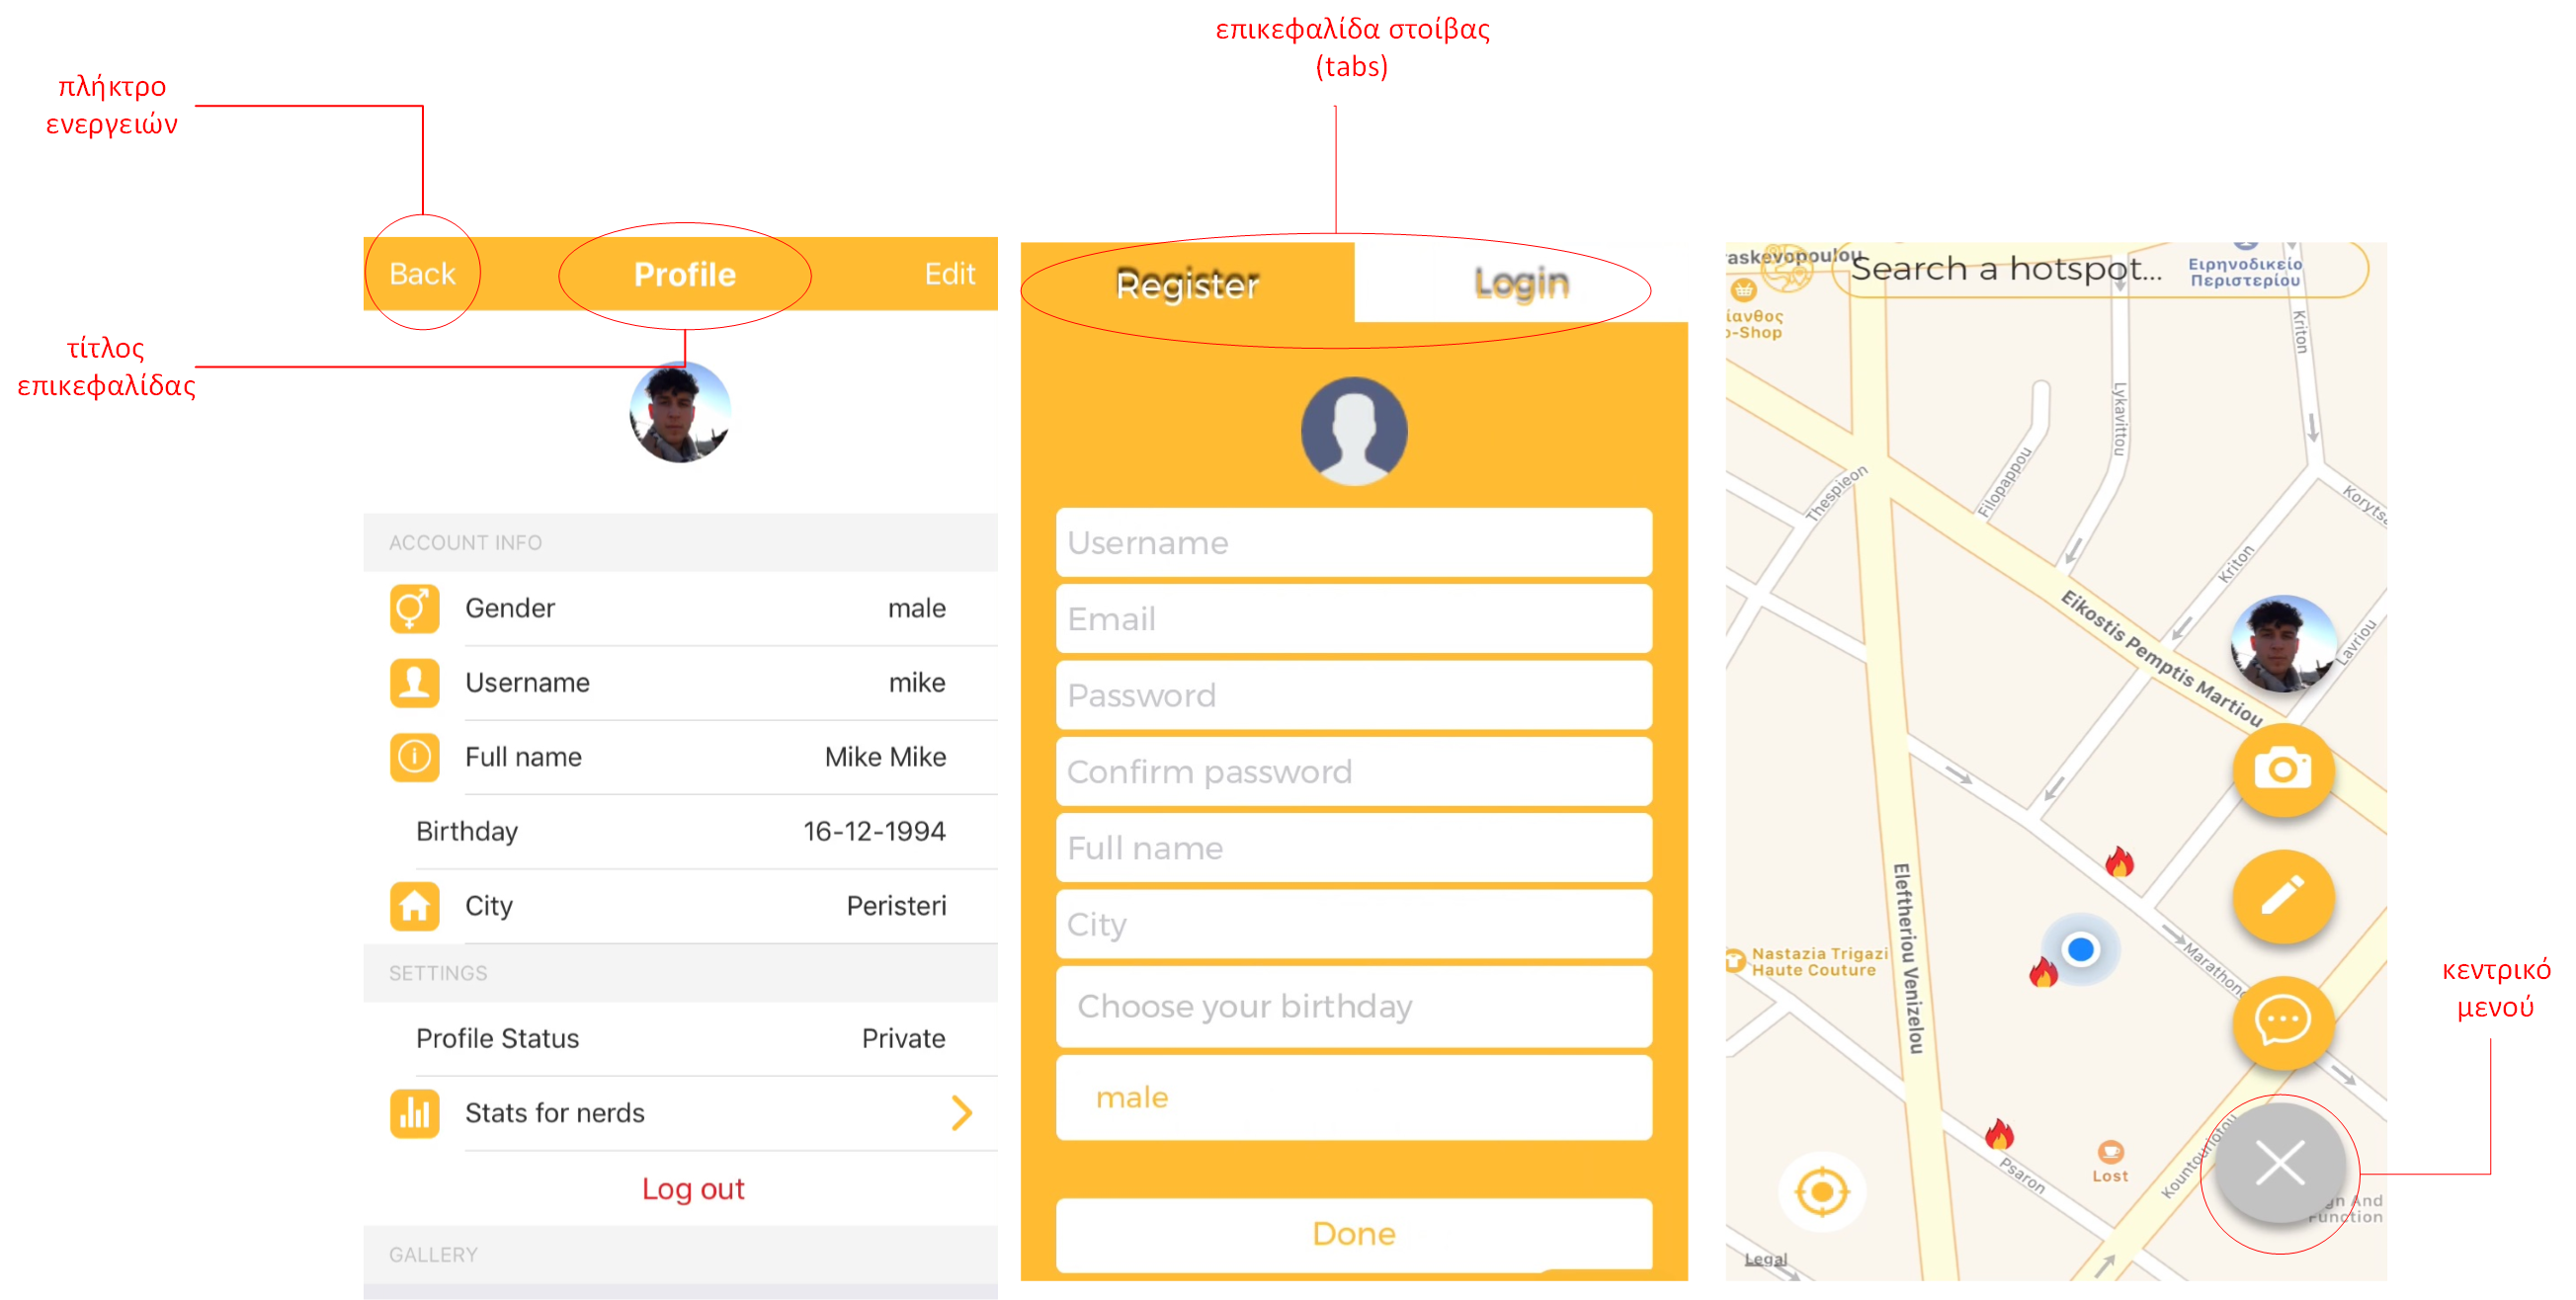
\includegraphics[scale=0.2]{figures/exaple.png}
    \caption{Παράδειγμα χαρακτηριστικών που επαναλαμβάνονται σε όλη την εφαρμογή.}
    \label{example}
\end{figure}

\subsubsection{Τεχνική Πλοήγησης στην Εφαρμογή}
Ένα από τα βασικότερα σημεία της υλοποίησης αποτελεί η πλοήγηση εντός της εφαρμογής. Η τεχνική που ακολουθήθηκε βασίζεται στην ύπαρξη ενός ενιαίου \tl{router}, ο οποίος είναι υπευθυνος για την πλόγηση κάθε φορά στην επιλεγμένμη σελίδα, αλλά και την αποθήκευση της σελίδας σε μια στοίβα. Με αυτό τον τρόπο, είναι δυνατή η εκτεταμένη περιήγηση σε περισσότερες από μια σελίδες της εφαρμογής και η επιστροφή σε οποιαδήποτε από τις προηγούμενες σελίδες χάρις την δυνατότητα διευθυνσιοδότητησης καθεμιάς από τις σελίδες αυτές.
\newline
\indent
Πρακτικά, αυτό επιτυγχάνεται με την τεχνική των εμφωλευμένων σελίδων. Σύμφωνα με αυτή, οι σελίδες που πρόκειται να έχουν τη δυνατότητα επιστροφής σε κάποια προηγούμενη σελίδα θα εμφωλιάζονται ομαδικά υπό μια υποτιθέμενη ``\textit{σκηνή}'' (\tl{scene}). Κάθε σελίδα αποτελεί από μόνη της μια σκηνή και πολλές σκηνές μαζί δημιουργούν μια ``\textit{στοίβα}'' από σκηνές (\tl{stack}). Όσες σκηνές βρίσκονται εντός της στοίβας, μπορούν να διαδέχονται η μία την αμέσως επόμενη, έχοντας ταυτόχρονα την δυνατότητα επιστροφής στην προηγούμενη σελίδα-σκηνή. Επίσης, υιοθετούν μία σειρά από ιδιότητες στις οποίες θα γίνει αναφορά στις ενότητες που ακολουθούν.
\newline
\indent
Όλες οι στοίβες που θα δημιουργηθούν τελικά, είναι εμφωλευμένες στον \tl{router}. Αν το τελευταίο δεν ισχύει, τότε οι παραπάνω ιδιότητες δεν εφαρμόζονται στις επιμέρους στοίβες.


\subsubsection{Επικεφαλίδα Οθόνης}
 Μία από τις βασικότερες ίσως ιδιότητες που μεταδίδεται στις σκηνές που απαρτίζουν μια στοίβα είναι η επικεφαλίδα. Κάθε οθόνη που ανήκει στην ομάδα εμφωλευμένων σκηνών έχει την δυνατότητα να φέρει ή όχι κάποια χαρακτηριστικά στην επικεφαλίδα. Αυτά είναι η επιπλέον επικεφαλίδα της στοίβας, αποκλειστικές σχεδιαστικές επεμβάσεις (όπως πχ. χρώμα, είδος και μέγεθος γραμματοσειράς, εικονίδια κλπ.),  ο τίτλος της παρούσας σελίδας, διαρρύθμιση πλήκτρων που θα έχει η επικεφαλίδα, αλλαγή θέσης των στοιχείων και πολλά άλλα. Η επικεφαλίδα αποτελεί ξεχωριστό \tl{component}, το οποίο ανήκει σε μια ομάδα επαναχρησιμοποιήσιμων \tl{components} (\tl{commons}) και χρησιμοποιείται σε κάθε σελίδα με διαφορετικές διαρρυθμίσεις.
 \newline
\indent
Οι παραπάνω ιδιότητες είναι ιδιαίτερα χρήσιμες στον προγραμματισμό κάθε οθόνης. Δίνουν πολλές επιλογές στον προγραμματιστή όσον αφορά στην διαμόρφωση της επικεφαλίδας της κάθε οθόνης και την ανεξαρτητοποίηση των οθονών μεταξύ τους από  σχεδιαστικής απόψεως. Από την άλλη, μπορούν να αυτοματοποιηθούν πολλές προγραμματιστικές ενέργειες με την χρήση τμημάτων κώδικα που μπορεί να επαναχρησιμοποιηθεί σε όλες σχεδόν τις οθόνες. Αυτό καθιστά τη διαδικασία προγραμματσιμού αισθητά πιο εύκολη και βέλτιση.

\subsubsection{Κεντρικό Μενού Οθονών}
Στη δεξιότερη εικόνα του σχ. \ref{example} φαίνεται το κεντρικό μενού για την πλοήγηση μεταξύ των οθονών της εφαρμογής. Η τεχνική χρήσης ενός κεντρικού πλήκτρου για όλες τις βασικές οθόνες της εφαρμογής επιλύει πολλά προβλήματα και καθιστά το κομμάτι του προγραμματισμού αρκετά πιο απλό. Το \tl{FAB} εξυπηρετεί επίσης από άποψη χώρου, αφού δεν καταλαμβάνει μεγάλο τμήμα της  κεντρικής οθόνης, πράγμα που το κάνει την καταλληλότερη προγραμματιστική τεχνική. Μια άλλη προσέγγιση θα ήταν η ύπαρξη μιας μπάρας εικονιδίων με τις κύριες οθόνες στο κάτω μέρος της οθόνης, αλλά αυτό θα μείωνε αρκετά τις διαστάσεις της διεπαφής χάρτη, που είναι άλλωστε και το κύριο χαρακτηριστικό της οθόνης.
\newline
\indent
Το \tl{FAB} αποτελεί ξεχωριστό \tl{component} της κεντρικής οθόνης και συνίσταται από το κύριο πλήκτρο επέκτασης του μενού και τρία επιμέρους εικονίδια. Κάθε εικονίδιο αντιστοιχεί και σε μία από τις βασικές οθόνες της εφαρμογής και για τον λόγο αυτό του έχει αποδωθεί κατάλληλο εικονίδιο.


\subsubsection{Βασικά Πλήκτρα Ενεργειών}
Όπως έχει ήδη αναφερθεί, κάθε οθόνη διαθέτει μια εξατομικευμένη επικεφαλίδα. Η επικεφαλίδα, εκτός των άλλων φέρει τον τίτλο της σελίδας στον οποίο βρίσκεται ο χρήστης και κάποια βασικά πλήκτρα ενεργειών. Τα πλήκτρα αυτά αποσκοπούν στην δυνατότητα πλοήγησης προς τα εμπρός ή προς τα πίσω σε μια στοίβα σελίδων. Για παράδειγμα, όταν ο χρήστης επισκέπτεται την οθόνη του προσωπικού του \tl{profile} (\tl{ProfileScreen}), μπορεί είτε να επιστρέψει στην προηγούμενη σελίδα πατώντας το πλήκτρο επιστροφής με την επιγραφή ``\textit{\tl{back}}'', είτε να πλοηγηθεί στην σελίδα επεξεργασίας των προσωπικών του στοιχείων (\tl{EditProfileScreen}) πατώντας το πλήκτρο επιστροφής με την επιγραφή ``\textit{\tl{edit}}''.
\newline
\indent
ο προγραμματισμός της λειτουργικότητας του κάθε πλήκτρου ενεργειών εξαρτάται από το είδος της σελίδας. Το πλήκτρο στα αριστερά μιας σελίδας έχει πάντοτε το ρόλο επιστροφής στην προηγούμενη σελίδα. Ανάλογα με τις ενέργειες που θα παρέχονται στον χρήστη, το πλήκτρο ενεργειών στα δεξιά της επικεφαλίδας θα εκτελεί είτε την λειτουργία επεξεργασίας δεδομένων, είτε τη λειτουργία υποβολής φόρμας. Στο παραπάνω παράδειγμα, η οθόνη στην οποία αναφέρονται τα πλήκτρα ενεργειών είναι αυτή του \tl{profile} του χρήστη, επομένως το πλήκτρο στα αριστερά παίζει το ρόλο της επιστροφής στην προηγούμενη σελίδα, ενώ το πλήκτρο στα δεξιά μεταφέρει το χρήστη στην οθόνη επεξεργασίας. Εκεί έπειτα, τα πλήκτρα αναφέρονται σε μια οθόνη που περιέχει φόρμα, συνεπώς το πλήκτρο στα δεξιά έχει τώρα τον ρόλο υποβολής της φόρμας. 

\subsection{Λειτουργικότητα Οθονών Εφαρμογής}
Στην ενότητα αυτή θα αναλυθούν οι μεθοδολογίες που ακολουθήθηκαν στην υλοποίηση των λειτουργικοτήτων της εφαρμογής. Όπως αναφέρθηκε ήδη στο Κεφ. 3, η εφαρμογή θα δίνει στο χρήστη τη δυνατότητα εγγραφής και σύνδεσης στην εφαρμογή, ως μέσο ταυτοποίησης. Ακόμη, ο χρήστης θα μπορεί να πλοηγείται σε ένα χάρτη στα διάφορα σημεία ενδιαφέροντος. Εκεί, θα μπορεί να επιλέξει από μια πληθώρα ενεργειών για να αλληλεπιδράσει με τα στοιχεία του χάρτη. Η εφαρμογή θα δίνει στο χρήστη τη δυνατότητα να εξατομικεύσει τον προσωπικό του λογαριασμό, μέσα από την ταξιθέτηση των προσωπικών του δημοσιεύσεων αλλά και από την επεξεργασία του προσωπικού του \tl{profile}. Τέλος, ο χρήστης θα μπορεί να αποσυνδεθεί απο την εφαρμογή όποτε το επιθυμεί.
 


\subsubsection{\tl{RegisterScreen \& LoginScreen}}
Η οθόνη αποτελείται από δύο επιμέρους \tl{tabs}, ένα για εγγραφή και ένα για σύνδεση των χρηστών. Ο χρήστης μπορεί να επιλέγει κάθε φορά το \tl{tab} που αρμόζει στην στην κάθε περίπτωση. Εάν ο χρήστης επιθυμεί να πραγματοποιήσει εγγραφή στην εφαρμογή, μπορεί να επιλέξει το \tl{tab} με τίτλο ``\textit{\tl{Register}}'', κάνοντας \tl{swipe} προς τα δεξιά. Από την άλλη, εάν ο χρήστης θέλει να πραγματοποιήσει σύνδεση στον λογαριασμό του, μπορεί να επιλέξει το \tl{tab} με τίτλο ``\textit{\tl{Login}}'', κάνοντας \tl{swipe} προς τα αριστερά.
\newline
\indent
Κάθε οθόνη περιέχει μια φόρμα με πεδία τα οποία καλείται να συμπληρώσει ο χρήστης. Στην οθόνη εγγραφής, η φόρμα περιέχει πεδία για το πλήρες όνομα, το όνομα χρήστη, την ηλεκτρονική διεύθυνση, τον κωδικό πρόσβασης, την πόλη, το γένος και την ημερομηνία γέννησης του χρήστη. Επίσης, ο χρήστης μπορεί να επιλέξει μία από τις φωτογραφίες στη συλλογή του ή να βγάλει μια νέα φωτογραφία και να την θέσει ως εικόνα προφίλ στο λογαριασμό του. Η οθόνη σύνδεσης είναι πιο σύντομη και αποτελείται από δύο πεδία, τα οποία ο χρήστης συμπληρώνει με τα διαπιστευτήριά του. Ο συνδυασμός διαπιστευτηρίων χρήστη αποτελείται από την ηλεκτρονική διεύθυνση και των κωδικό πρόσβασης του χρήστη. Σε καθεμία εκ των ανωτέρω περιπτώσεων, ο χρήστης μεταφέρεται στο χάρτη της κεντρικής οθόνης της εφαρμογής μετά από επιτυχή υποβολή της φόρμας.
\newline
\indent
Κάθε φόρμα έχει υλοποιηθεί ώστε να προσφέρει την καλύτερη δυνατή εμπειρία χρήστη. Το είδος της εισόδου που απαιτείται στην συμπλήρωση κάθε φόρμας διαφέρει από πεδίο σε πεδίο. Για παράδειγμα, το πεδίο κωδικού πρόσβασης απαιτεί είσοδο αποτελούμενη από αλφαριθμητικούς χαρακτήρες, ενώ στο πεδίο της ηλεκτρονικής διεύθυνσης χρησιμοποιούνται συγκεκριμένοι ειδικοί χαρακτήρες και σύμβολα. Για το λόγο αυτό, έχει προσιοριστεί το είδος κάθε πεδίου, με αποτέλεσμα την εμφάνιση του κατάλληλου είδους πληκτρολογίου κάθε φορά. Επίσης, το πλήκτρα υποβολής κάθε φόρμας αντικαθίστανται από \tl{spinners} που δείχνουν στο χρήστη ότι η εφαρμογή φορτώνει.
\newline
\indent
Σε περίπτωση ανεπιτυχούς υποβολής κάποιας από τις παραπάνω φόρμες, η εφαρμογή ενημερώνει το χρήστη σχετικά με τη φύση του σφάλματος. Σφάλματα μπορούν να προκύψουν από την λανθασμένη συμπλήρωση ενός ή περισσότερων πεδίων εισόδου. Σε κάθε περίπτωση, ένα κατάλληλο μήνυμα λάθους εμφανίζεται κάτω από το αντίστοιχο πεδίο, το οποίο αναφέρει συνοπτικά τις μετατροπές που πρέπει να γίνουν ώστε να είναι αποδεκτή η είσοδος του χρήστη. 

\subsubsection{\tl{HomeScreen}}

Σε αυτό το σημείο της εφαρμογής εμφανίζονται και οι κατάλληλες ειδοποιήσεις στο χρήστη. Η εφαρμογή χρείαζεται την τοποθεσία του χρήστη για να την προσδιορίσει στο χάρτη και στη συνέχεια να φορτώσει τα \tl{hotspots}. Δίνοντας την συγκατάνευσή του, ο χρήστης επιτρέπει στην εφαρμογή να πραγματοποιήσει τις αναγκαίες ρυθμίσεις για την ορθή λειτουργία της. Επίσης, ο χρήστης θα πρέπει να πραγματοποιήσει σύνδεση σε κάποιο δίκτυο προκειμένου να μπορέσει να χρησιμοποιήσει την εφαρμογή.
\newline
\indent
Μετά την είσοδό του στην εφαρμογή, ο χρήστης ανακατευθύνεται στον χάρτη. Ο χάρτης φορτώνει με τα \tl{hotspots} που βρίσκονται εντός εμβέλειας της τοποθεσίας του χρήστη. Η εμβέλεια είναι προγραμματισμένη να έχει μία ακτίνα ίση με \tl{5km}. Τα \tl{hotspots} που φαίνονται στο χάρτη και έχουν δημιουργηθεί από άλλους χρήστες συμβολίζονται με \tl{markers} που έχουν τη μορφή φωτιάς συγκεκριμένου μεγέθους. Το μέγεθος κάθε \tl{marker} ποικίλλει και εξαρτάται από τον αριθμό προβολών του \tl{hotspot}. Οσο πιο πολλοί χρήστες έχουν δει ένα συγκεκριμένο \tl{hotspot}, τόσο μεγαλύτερο είναι το μέγεθος της φωτιάς. Έτσι, δημιουργείται μια αναλογία μεταξύ των \tl{hotspots} και του ενδιαφέροντος των χρηστών.
\newline
\indent
Ο χρήστης μπορεί να επιλέξει να προβάλλει ένα \tl{hotspot} από το χάρτη. Πατώντας επάνω στο \tl{marker} του \tl{hotspot}, θα εμφανιστεί ένα πλαίσιο (\tl{callout}), το οποίο περιέχει τις κυριότερες πληροφορίες που σχετίζονται με το συγκεκριμένο \tl{hotspot}. Στο πλαίσιο φαίνεται συνοπτικά ένα τμήμα της περιγραφής του \tl{hotspot}, το όνομα και η εικόνα προφίλ του χρήστη που έχει αναρτήσει το \tl{hotspot}, ο χρόνος που έχει περάσει από την ώρα ανάρτησης, και ο αριθμός προβολών και σχολίων του \tl{hotspot}. 
\newline
\indent
Στην οθόνη χάρτη υπάρχουν τέσσερεις επιπλέον διεπαφές. Η μπάρα αναζήτησης, το κρυφό συρταρωτό μενού, το πλήκτρο επαναφοράς τοποθεσίας χρήστη και το κεντρικό πλήκτρο πλοήγησης. Το πλήκτρο επαναφοράς τοποθεσίας χρήστη βρίσκεται στο κάτω αριστερά μέρος της οθόνης. Όπως φανερώνει και το όνομά του, βοηθάει το χρήστη να επαναφέρει τη θέση του χάρτη στην τοποθεσία την οποία βρίσκεται εκείνη τη στιγμή. Το κεντρικό πλήκτρο πλοήγησης βρίσκεται στο κάτω δεξιά μέρος της οθόνης και πατώντας το ο χρήστης μπορεί να επιλέξει σε ποια οθόνη θέλει να μεταφερθεί. Για τις άλλες δύο διεπαφές θα γίνει μια πιο εκτεταμένη αναφορά στη συνέχεια. 

\paragraph{Μπάρα Αναζήτησης και \tl{Foursquare Suggest Completion}}
\paragraph{}
Εάν ο χρήστης επιθυμεί να πραγματοποιήσει μια συγκεκριμένη αναζήτηση ενός σημείου ενδιαφέροντος, μπορεί να το κάνει μέσω της μπάρας αναζήτησης στο πάνω μέρος της οθόνης. Ο χρήστης πληκτρολογεί λέξεις-κλειδιά που σχετίζονται με την τοποθεσία προς αναζήτηση, όπως το όνομα, την περιοχή κλπ. Η διεπαφή είναι εφοδιασμένη με την ιδιότητα αυτοσυμπλήρωσης του \tl{Foursquare API}. Συνεπώς, τα αποτελέσματα εμφανίζονται καθώς ο χρήστης πληκτρολογεί, σε μια λίστα ακριβώς κάτω από την μπάρα. 
\newline
\indent
 Το \tl{Foursquare API}, όπως αναφέρθηκε στην ενότητα 2.2.2, είναι μια διεπαφή ανοικτού κώδικα η οποία χρησιμεύει στην εύρεση πληροφοριών για διάφορα μέρη. Στην εφαρμογή, ένα από τα σημεία στα οποία ενσωματώνεται η διεπαφή αυτή είναι η μπάρα αναζήτησης στο επάνω μέρος του χάρτη, για την αυτοσυμπλήρωση των εμφανιζόμενων αποτελεσμάτων. Όταν πραγματοποιείται αναζήτηση, η είσοδος του χρήστη προστίθεται στο προς αναζήτηση \tl{URL} και η εφαρμογή δημιουργεί ένα αίτημα \tl{GET} προς την διεπαφή \tl{Foursquare API Suggest Completion}
 
\hfill
\begin{mdframed}[backgroundcolor=lightgrey] 
 \tl{\ttfamily{GET https://api.foursquare.com/v2/venues/suggestcompletion}}   
\end{mdframed}
\hfil

\noindent  επισυνάπτοντας τις λέξεις-κλειδιά και κάποια ακόμη δεδομένα ως \tl{endpoint} στο παραπάνω \tl{URL}, για την λήψη των απαιτούμενων πληροφοριών του σημείου ενδιαφέροντος. Το αποτέλεσμα είναι η εμφάνιση προτεινόμενων σημείων ανδιαφέροντος καθώς ο χρήστης πληκτρολογεί την επιθυμητή είσοδο.  

Το αίτημα που τελικά αποστέλλεται στο \tl{Foursquare API} αποτελείται από ένα νέο \tl{URL}, το οποίο περιλαμβάνει τα απαραίτητα στοιχεία για την εύρεση των σχετικών αποτελεσμάτων. Το νέο \tl{URL} που δημιουργείται, εμπεριέχει το παραπάνω \tl{URL}, μαζί με ένα \tl{query} που περιλαμβάνει τις εξής παραμέτρους αναζήτησης:

\begin{itemize}
    \item \textbf{\textit{\tl{ll}}} \textbf{--} η παράμετρος αυτή προσδιορίζει την τοποθεσία στην οποία γίνεται η αναζήτηση
    \item \textbf{\textit{\tl{query}}} \textbf{--} οι λέξεις-κλειδιά που πληκτρολογεί ο χρήστης
    \item \textbf{\textit{\tl{limit}}} \textbf{--} η παράμετρος αυτή προσδιορίζει την πλήθος των εμφανιζόμενων αποτελεσμάτων
    \item \textbf{\textit{\tl{radius}}} \textbf{--} η παράμετρος αυτή προσδιορίζει την ακτίνα αναζήτησης σε \tl{m}
    \item \textbf{\textit{\tl{v}}} \textbf{--} η παράμετρος αυτή προσδιορίζει την \tl{version} της διεπαφής
\end{itemize}


Στον πίνακα που ακολουθεί, γίνεται ανάλυση ενός παραδείγματος για την καλύτερη κατανόηση του τρόπου λειτουργίας της διεπαφής αυτοσυμπλήρωσης.

\begin{table}[h]
\centering
\begin{tabular}{ |m{2cm}|m{2cm}|m{8cm}|  }
\hline
\multicolumn{3}{|c|}{\selectlanguage{english}Search Example: Acropolis Museum\selectlanguage{greek}} \\
\hline 
\textit{\tl{\textbf{Name}}} & \textit{\tl{\textbf{Example}}} & \textit{\tl{\textbf{Description}}}  \\
\hline 
\tl{\textit{ll}}
 & \tl{37.8,23.2} & \tl{\textbf{required} latitude and longitude of the user’s location.}\\
\hline
\tl{\textit{query}}
 & \tl{acropolis museum} & \tl{\textbf{required} search term to be applied against titles. Must be at least 3 characters long.}\\
 \hline
 \tl{\textit{limit}}
 & \tl{20} & \tl{number of results to return, up to 50.}\\
 \hline
 \tl{\textit{radius}}
 & \tl{800} & \tl{limit results to venues within this many meters of the specified location. Defaults to a city-wide area. The maximum supported radius is currently 80,000 meters.}\\
\hline
 \tl{\textit{v}}
 & \tl{20190501} & \tl{the current API version.}\\
\hline
 \tl{\textit{client\_id}}
 &  & \tl{a \textbf{unique} string that is given to the client for access privileges.}\\
\hline
 \tl{\textit{client\_secret}}
 &  & \tl{a \textbf{unique} string that is given to the client for access privileges.}\\
\hline
\end{tabular}
\selectlanguage{greek}
\caption{Παράδειγμα αυτοσυμπλήρωσης για τις λέξεις-κλειδιά \tl{acropolis museum} και δομή του \tl{URL} αναζήτησης.}
\label{tab:parameters}
\end{table}


\paragraph{Συρταρωτό Μενού και \tl{Foursquare Explore}}
\paragraph{}
Στις δυνατότητες του χρήστη συμπεριλαμβάνεται και η φιλτραρισμένη αναζήτηση σημείων ενδιαφέροντος. Εάν ο χρήστης επιθυμεί να προβάλλει στο χάρτη σημεία που ανήκουν σε κάποια συγκεκριμένη κατηγορία, μπορεί να το κάνει, ανοίγοντας το κρυφό συρταρωτό μενού πατώντας το εικονίδιο της υδρόγειου σφαίρας στο επάνω αριστερά μέρος του χάρτη, ή σύροντας την οθόνη προς τα δεξιά. Στη συνέχεια, μπορεί να επιλέξει μία από τις κατηγορίες της λίστας και τα αποτελέσματα θα εμφανιστούν στο χάρτη. 
\newpage
Η παραπάνω υπηρεσία υλοποιείται με τη χρήση της διεπαφής \tl{Foursquare Explore}, με βάση την οποία η εφαρμογή δημιουργεί αιτήματα αναζήτησης σημείων ενδιαφέροντος που ανήκουν σε κάποια από τις διαθέσιμες κατηγορίες. Τα αιτήματα που δημιουργούνται έχουν την ακόλουθη μορφή

\begin{mdframed}[backgroundcolor=lightgrey] 
 \tl{\ttfamily{GET https://api.foursquare.com/v2/venues/search}}   
\end{mdframed}

\noindent και το \tl{URL} εμπεριέχει κάποιες επιπρόσθετες παραμέτρους που συνιστούν το \tl{query} προς αποστολή στην διεπαφή. Στη συνέχεια θα αναλυθεί ένα παράδειγμα των αποτελεσμάτων που επιστρέφονται στην εφαρμογή από τη διεπαφή, όταν ο χρήστης επιλέγει την κατηγορία με ετικέτα ``\textit{\tl{arts}}''.
\newline
\indent
Το νέο \tl{URL} που θα δημιουργηθεί θα ξεκινάει με το παραπάνω \tl{URL} και θα περιέχει κάποιες ακόμη πληροφορίες που θα συνιστούν το τελικό \tl{endpoint}. Οι πληροφορίες αυτές είναι παρόμοιες με αυτές που χρησιμοποιήθηκαν για το σχηματισμό του \tl{endpoint} που θα αποσταλλεί στη διεπαφή \tl{Foursquare Suggest Completion}, με μία μόνο επιπλέον παράμετρο: την κατηγορία (\tl{section}) στην οποία ανήκει το σημείο ενδιαφέροντος, για τον περιορισμό της αναζήτησης. Στο παράδειγμα όπου ο χρήστης επιλέγει σαν φίλτρο της αναζήτησης την κατηγορία ``\textit{\tl{arts}}'', τότε η παράμετρος \tl{section} αντιστοιχίζεται με την κατηγορία \tl{arts}.
\newline
\indent
Τα αποτελέσματα που επιστρέφει η διεπαφή \tl{Foursquare Explore} θα περιέχουν μια σειρά από πληροφορίες, τις οποίες η εφαρμογή θα διαχειρίζεται κατάλληλα για την εμφάνισή τους στο χάρτη. Τα στοιχεία που επιστρέφονται από τη διεπαφή φαίνονται στον κάτωθι πίνακα:

\begin{table}[h]
\centering
\begin{tabular}{ |m{2cm}|m{10cm}|  }
\hline
\multicolumn{2}{|c|}{\tl{https://api.foursquare.com/v2/venues?ll=37.8,23.7\&section=arts\&radius=800}} \\
\hline 
\textit{\tl{\textbf{Field}}} & \textit{\tl{\textbf{Description}}}  \\
\hline 
\tl{\textit{id}}
 & \tl{a \textbf{unique} string identifier for this venue.}\\
\hline
\tl{\textit{name}}
 & \tl{the best known name for this venue.}\\
 \hline
 \tl{\textit{location}}
 & \tl{an object containing none, some, or all of address (street address), crossStreet, city, state, postalCode, country, lat, lng, and distance. All fields are strings, except for lat, lng, and distance. Distance is measured in meters. Some venues have their locations intentionally hidden for privacy reasons (such as private residences). If this is the case, the parameter isFuzzed will be set to true, and the lat/lng parameters will have reduced precision.}\\
 \hline
 \tl{\textit{categories}}
  & \tl{an array, possibly empty, of categories that have been applied to this venue. One of the categories will have a primary field indicating that it is the primary category for the venue. For the complete category tree, see categories.}\\
\hline
\end{tabular}
\selectlanguage{greek}
\caption{πληροφορίες που επιστρέφονται από τη διεπαφή \tl{Foursquare Explore}.}
\label{tab:parameters}
\end{table}

Εκτός από την αναζήτηση σημείων ενδιαφέροντος, ο χρήστης μπορεί να προβάλλει κάποια από τα \tl{hotspots} που εμφανίζονται στο χάρτη. Πατώντας επάνω σε κάποιο \tl{marker}, ο χρήστης μπορεί να δει τις πληροφορίες που αφορούν το συγκεκριμένο \tl{hotspot}, όπως να διαβάσει την περιγραφή, να δει το χρήστη που δημιούργησε το \tl{hotspot}, να δει τον αριθμό σχολίων ή προβολών κλπ. 


\subsubsection{\tl{CreateHotspotScreen}}
Για τη δημιουργία ενός προσωπικού \tl{hotspot}, ο χρήστης μεταφέρεται στην οθόνη \tl{CreateHotspotScreen}. Εκεί, μπορεί να δώσει στο νέο του \tl{hotspot} μια περιγραφή, να θέσει χρόνικό όριο ισχύος και να επισυνάψει μια φωτογραφία από τη συλλογή της συσκευής του ή να βγάλει καινούρια με την κάμερα. Μόλις ολοκληρώσει τη συμπλήρωση της φόρμας δημιουργίας με τα παραπάνω στοιχεία, ο χρήστης πατάει το πλήκτρο με επιγραφή ``\textit{\tl{Done}}'' που βρίσκεται στο δεξιά μέρος της επικεφαλίδας της οθόνης.
\newline
\indent
Σε περίπτωση σφάλματος, η διεπαφή μηνυμάτων λάθους αναλαμβάνει την εμφάνιση κατάλληλου μηνύματος προς το χρήστη. Το μήνυμα θα έχει τη μορφή ειδοποιητικού πλαισίου διαλόγου, όπου και θα περιγράφεται το αίτιο που προξενεί το σφάλμα στη φόρμα δημιουργίας \tl{hotspot}. Στη συνέχεια, ο χρήστης αποδέχεται την ειδοποίηση πατώντας ``\textit{\tl{OK}}'' και προχωράει στη διόρθωση των σφαλμάτων. Το πεδίο περιγραφής του \tl{hotspot} δεν πρέπει να είναι κενό, ενώ η τιμή χρονικού ορίου αρχικοποιείται στα 30 λεπτά. Η προσθήκη φωτογραφίας είναι προαιρετική. Ο χρήστης μπορεί να ακυρώσει τη δημιουργία του νέου \tl{hotspot} ανά πάσα στιγμη πατώντας το πλήκτρο με επιγραφή ``\textit{\tl{Cancel}}'' που βρίσκεται στα αριστερά της επικεφαλίδας της οθόνης.
\newline
\indent
Μόλις η φόρμα δημιουργίας νέου \tl{hotspot} διορθωθεί και δεν περιέχει άλλα λάθη, η υποβολή ολοκληρώνεται επιτυχώς. Ο χρήστης ενημερώνεται για τις ενέργειες που θα ακολουθήσουν μετά την υποβολή της φόρμας και καλείται να αποδεχθεί ή όχι την δημιουργία του νέου \tl{hotspot}. Εάν ο χρήστης αποδεχθεί τη δημιουργία του νέου \tl{hotspot}, τότε ανακατευθύνεται στο χάρτη και το καινούριο \tl{hotspot} αποθηκεύεται στη βάση και εμφανίζεται στο χάρτη στην τοποθεσία του χρήστη. Διαφορετικά, το \tl{hotspot} δεν αποθηκεύεται και ο χρήστης μεταφέρεται ξανά στο χάρτη.


\subsubsection{\tl{HotspotListScreen}}
Η εξατομίκευση της εφαρμογής ανάλογα με το χρήστη επιτυγχάνεται με την λίστα προσωπικών \tl{hotspots} στην \tl{HotspotListScreen}. Εκεί, μπορεί να μεταφερθεί ο χρήστης όταν επιθυμεί να προβάλλει όλα τα προσωπικά \tl{hotspots} που έχει δημιουργήσει στο παρελθόν. Η λίστα είναι ταξινομημένη με τα πιο πρόσφατα  \tl{hotspots} να εμφανίζονται πρώτα και τα παλαιότερα να βρίσκονται στο τέλος. 
\newline
\indent
Η οθόνη προσωπικών  \tl{hotspots} εξυπηρετεί επίσης στην διευκόλυνση της διαδικασίας διαχείρισης των  \tl{hotspots} του χρήστη. Εάν ο χρήστης επιθυμεί να επεξεργαστεί την περιγραφή κάποιου \tl{hotspot} για παράδειγμα, μπορεί να το κάνει από εδώ. Η διαδικασία είναι απλή και σύντομη, αφού ο χρήστης απλώς σύρει το συγκεκριμένο \tl{hotspot} προς τα δεξιά και πατάει το πλήκτρο με την επιγραφή ``\tl{\textit{edit}}''. Στην σελίδα επεξεργασίας, ο χρήστης μπορεί να μεταβάλλει όλες τις πληροφορίες που σχετίζονται με το \tl{hotspot}. Μπορεί επίσης να αλλάξει την εικόνα του \tl{hotspot}, ή να προσθέσει μια εικόνα σε περίπτωση που δεν υπήρχε προηγουμένως. Επιπλέον, ο χρήστης μπορεί να διαγράψει όποιοδήποτε \tl{hotspot}. Η διαδικασία είναι παρόμοια με αυτή της την επεξεργασίας: ο χρήστης σύρει το \tl{hotspot} προς διαγραφή προς τα αριστερά και πατάει το πλήκτρο με την επιγραφή ``\tl{\textit{delete}}''.



\subsubsection{\tl{CommentScreen}}
Ο χρήστης μπορεί να αλληλεπιδράσει με ένα οποιοδήποτε \tl{hotspot}. Αυτό μπορεί να γίνει είτε από το χάρτη, είτε από τη λίστα προσωπικών \tl{hotspots}. Και στις δυο περιπτώσεις, ο χρήστης πατάει στο εικονίδιο με επιγραφή ``\tl{\textit{comments}}'' ενός \tl{hotspot} και μεταφέρεται αυτόματα στην οθόνη σχολίων. 
\newline
\indent
Από τη διεπαφή χάρτη, ο χρήστης μπορεί να αλληλεπιδράσει είτε με δικά του \tl{hotspots}, είτε με \tl{hotspots} άλλων χρηστών. Στην \tl{CommentScreen}, ο χρήστης μπορεί να διαβάσει την περιγραφή του \tl{hotspot}, να διαβάσει τα σχόλια των άλλων χρηστών, να προβάλλει την φωτογραφία του \tl{hotspot} εάν αυτή υποάρχει και να απαντήσει στο \tl{hotspot} γράφοντας το δικό του σχόλιο. Για να το κάνει αυτό, ο χρήστης περιηγείται στο κάτω μέρος της σελίδας, σύροντας την οθόνη προς τα πάνω. Εκεί μπορεί να εισάγει το σχόλιό του στο ειδικά διαμορφωμένο για αυτό το σκοπό τμήμα δημιουργίας σχολίων. Αφού ολοκληρώσει το σχόλιό του, ο χρήστης πατάει το πλήκτρο αποστολής που βρίσκεται στα δεξιά του \tl{reply box} και το νέο σχόλιο εμφανίζεται τελευταίο.
\newline
\indent
Η ίδια διαδικασία μπορεί να επιτευχθεί και από την \tl{HotspotListScreen}. Αυτή η μέθοδος συμφέρει περισσότερο εάν πρόκειται για κάποιο προσωπικό \tl{hotspot} του χρήστη.

\subsubsection{\tl{ProfileScreen}}
Ένα από τα σημαντικότερα χαρακτηριστικά της εφαρμογής είναι η οθόνη προσωπικού λογαριασμού του χρήστη. Η \tl{ProfileScreen} προσθέτει έναν ακόμη βαθμό εξατομίκευσης της εφαρμογής. Ο χρήστης μπορεί να προβάλλει πληροφορίες σχετικά με τη δράση του εντός της εφαρμογής, να δει ολόκληρη τη συλλογή φωτογραφιών που έχει δημιουργήσει και να επεξεργαστεί τις προσωπικές του πληροφορίες και ρυθμίσεις. 
\newline
\indent
Για την επεξεργασία των προσωπικών του στοιχείων και ρυθμίσεων, ο χρήστης πρέπει πρώτα να μεταφερθεί στην οθόνη επεξεργασίας του προσωπικού προφίλ. Αυτό επιτυγχάνεται πατώντας το πλήκτρο με την επιγραφή ``\tl{\textit{edit}}'' που βρίσκεται στα δεξιά του τίτλου της επικεφαλίδας της οθόνης. Έπειτα, ο χρήστης μεταφέρεται αυτόματα σε νέα σελίδα όπου υπάρχει μια φόρμα με τα παλιά στοιχεία του χρήστη. Με κατάλληλες περιγραφές των πεδίων, ο χρήστης καθοδηγείται στον τρόπο συμπλήρωσης της φόρμας επεξεργασίας προσωπικού προφίλ. Τα στοιχεία που μπορεί να επεξεργαστεί ο χρήστης είναι το πλήρες όνομα, το όνομα χρήστη, η ηλεκτρονική διεύθυνση, ο κωδικός πρόσβασης, η πόλη, η ημερομηνία γέννησης και το γένος. Επίσης, ο χρήστης μπορεί να αλλάξει την φωτογραφία προφίλ του. Εάν δεν υπάρχει φωτογραφία προφίλ, ο χρήστης μπορεί να προσθέσει μία από την συλλογή της συσκευής ή να βγάλει μια καινούρια με την κάμερα. Τέλος, ο χρήστης μπορεί να αλλάξει τις ρυθμίσεις του λογαριασμού του, από δημόσιο σε ιδιωτικό.
\newline
\indent
Σε περίπτωση σφάλματος, η διεπαφή μηνυμάτος λάθους αναλαμβάνει την καθοδήγηση του χρήστη για την διόρθωση των σφαλμάτων της φόρμας επεξεργασίας προφίλ. κατάλληλα μηνύματα λάθους εμφανίζονται κάτω από τα αντίστοιχα πεδία στα οποία έχει γίνει το λάθος. Τα μηνύματα εξαφανίζονται με την επίλυση του προβλήματος. Για την επιτυχή ολοκλήρωση της διαδικασίας επεξεργασίας του προσωπικού του προφίλ, ο χρήστης πρέπει να εισάγει τον κωδικό πρόσβασης. Στη συνέχεια, μεταφέρεται στο προφίλ του, όπου και τα στοιχεία του έχουν ανανεωθεί.
\newline
\indent
Η οθόνη προσωπικού λογαριασμού του χρήστη χρησιμεύει επίσης για την προβολή των στατιστικών δεδομένων. Ο χρήστης πατάει το βέλος που βρίσκεται στα δεξιά της επιγραφής ``\tl{\textit{Stats for nerds}}'', κάτω από το τμήμα ``\tl{\textit{SETTINGS}}''. Στη συνέχεια, ο χρήστης μεταφέρεται αυτομάτως σε νέα σελίδα, όπου υπάρχουν τρία τμήματα με στατιστικά δεδομένα. Στο πρώτο τμήμα με τίτλο ``\tl{\textit{ΑCCOUNT}}'' είναι συγκεντρωμένες οι πληροφορίες που αφορούν τη δράση του χρήστη εντός της εφαρμογής. Τα δεδομένα αυτά αφορούν τον αριθμό \tl{hotspots}, τον αριθμό προβολών και τον αριθμό σχολίων του χρήστη. Στο δεύτερο τμήμα με τίτλο ``\tl{\textit{INSIGHTS}}'' βρίσκονται τα ποσοστά που αφορούν την πορεία του χρήστη στην εφαρμογή. Τα ποσοστά αυτά σχετίζονται με το βαθμό δημοτικότητας που έχει αποκτήσει ο χρήστης σε σχέση με το υπόλοιπο σύνολο. Τέλος, στο τρίτο τμήμα με τίτλο ``\tl{\textit{AUDIENCE}}'', βρίσκονται τα ποσοστά των χρηστών με βάση το φύλο. 
\newline
\indent
Ο χρήστης μεταβαίνει στην \tl{ProfileScreen} και για την έξοδο από την εφαρμογή. Για να γίνει αυτό, ο χρήστης πρέπει να πατήσει το πλήκτρο που βρίσκεται κάτω από το τμήμα ``\tl{\textit{SETTINGS}}'', με την επιγραφή ``\tl{\textit{Log out}}'' με κόκκινους χαρακτήρες.

\subsection{Τενικές Ενιαίας Διαχείρισης Δεδομένων}
Στην εφαρμογή χρησιμοποιήθηκε μια τεχνολογία διαχείρισης δεδομένων για το συγχρονισμό μεταξύ των διαφόρων οθονών. Αυτό επιτεύχθηκε με την ενσωμάτωση της βιβλιοθήκης \tl{React Redux} και παρεμφερών εργαλείων που διευκολύνουν την διαδικασία ροής δεδομένων εντός της εφαρμογής, προσφέροντας επιπρόσθετες δυνατότητες στον προγραμματιστή. Χαρακτηριστικότερη εξ' αυτών είναι η αποθήκευση δεδομένων σε έναν ενιαίο χώρο, στον οποίο έχουν πρόσβαση όλα τα τμήματα της εφαρμογής τα οποία είναι συνδεδεμένα κατά κάποιο τρόπο με το χώρο αυτό. Στις ενότητες που ακολουθούν θα γίνει μια πιο εκτεταμένη ανάλυση των εργαλείων διαχείρισης που χρησιμοποιήθηκαν στην εφαρμογή.


\subsubsection{\tl{React Redux}}
Η \tl{React Redux} είναι μια βοηθητική βιβλιοθήκη ανοικτού κώδικα η οποία χρησιμεύει στην διαρρύθμιση των δεδομένων και την ιεράρχιση των καταστάσεων μιας εφαρμογής. Η ιδεολογία της βιβλιοθήκης αποτελεί έμπνευση της ομάδας προγραμματιστών του \tl{Facebook} και μιμείται τα χαρακτηριστικά μιας παρόμοιας βιβλιοθήκης, της \tl{Flux}. 

\begin{figure}
    \centering
    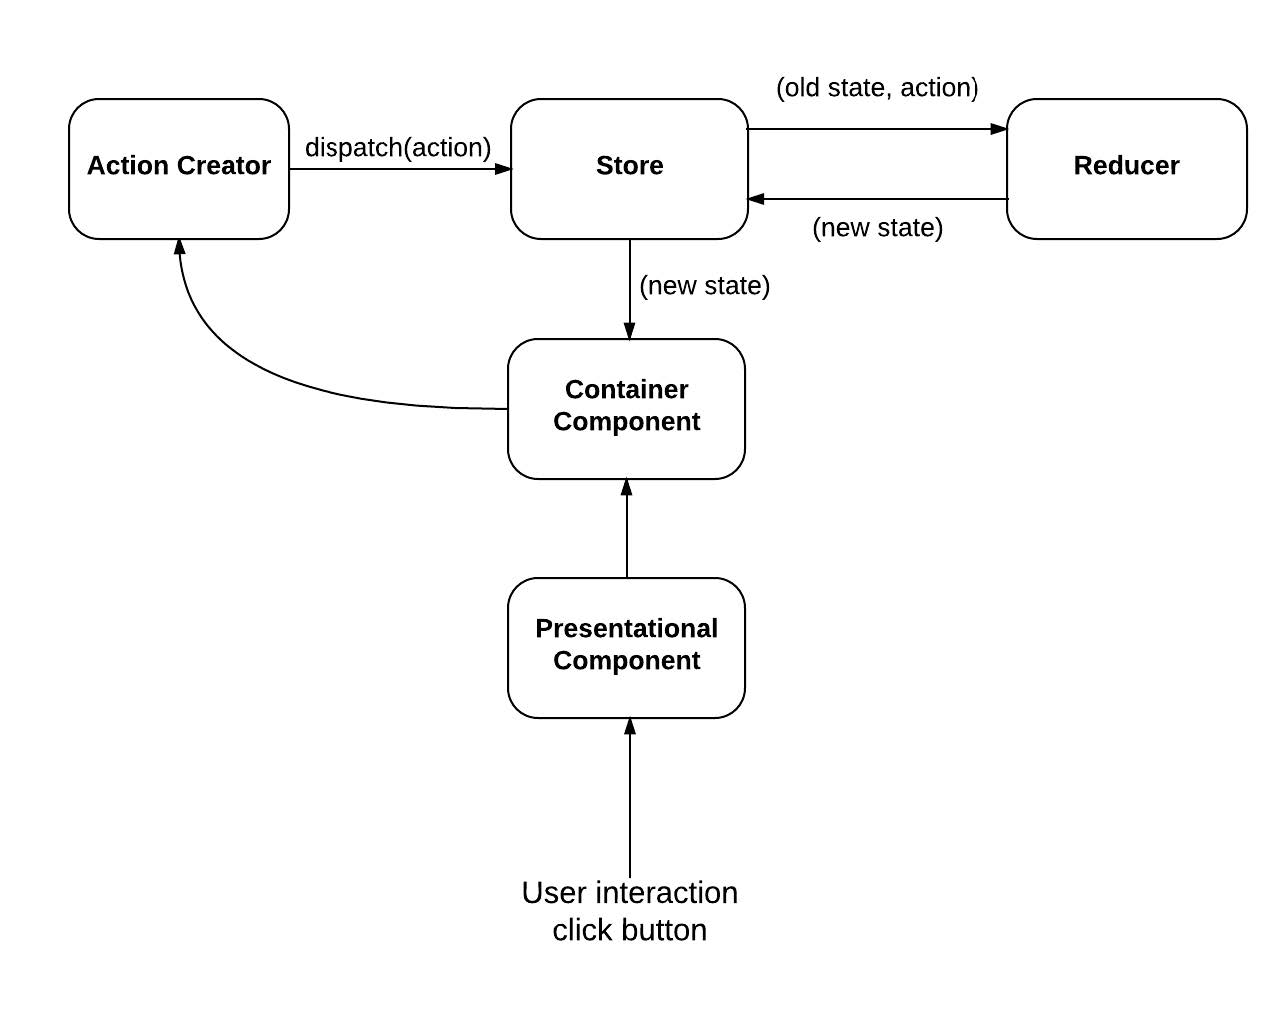
\includegraphics[scale=0.7]{figures/react-redux.png}
    \caption{Δομή \tl{React Redux} εντός της εφαρμογής.}
    \label{redux}
\end{figure}


Το κυριότερο πλεονέκτημα της \tl{React Redux} είναι ο τρόπος με τον οποίο διαχειρίζεται τα δεδομένα μιας εφαρμογής. Διαθέτει μια αμφίδρομη ροή δεδομένων μεταξύ ενός ενιαίου αποθηκευτικού χώρου και της εφαρμογής. Αυτό επιτρέπει στον προγραμματιστή τον εύκολο και γρήγορο τρόπο ανάπτυξης και αποσφαλμάτωσης της εφαρμογής.
\newline
\indent
Η δομή της εφαρμογής με τη χρήση της \tl{React Redux} φαίνεται στο σχ. \ref{redux}. Στη συνέχεια, ακολουθεί μια ανάλυση κάθε παράγοντα της βιβλιοθήκης, όπως αυτός χρησιμοποιείται εντός της εφαρμογής.

 \paragraph{\tl{\textbf{Presentational \& Container Components}}}
 \paragraph{}
 Κατά την υλοποίηση της εφαρμογής, κάθε οθόνη διακριτοποιείται σε στοιχεία αναπαράστασης δεδομένων (\tl{presentational/functional or stateless components}) και στοιχεία κατάστασης (\tl{container or ctateful components}), όπως έχει ήδη αναφερθεί στην ενότητα 4.1.4. Τα \tl{presentational components} δεν διαθέτουν λογική, το οποίο σημαίνει πως δε διαχειρίζονται καθόλου δεδομένα. Το μοναδικό συστατικό απαραίτητο στην λειτουργία τους είναι τα δεδομένα που λαμβάνουν μέσω των \tl{props} από το στοιχείο-πατέρα. Στην περίπτωση που απαιτείται η εκτέλεση μιας ενέργειας σχετική με τη διαζείριση δεδομένων από ένα \tl{presentational component}, αυτό επιτυγχάνεται με τον ίδιο τρόπο που λαμβάνονται τα δεδομένα. Με το ``\textit{πέρασμα}'' της αντίστοιχης συνάρτησης ανάκλησης (\tl{callback}) μέσω των \tl{props}, αυτή καθίσταται διαθέσιμη ανά πάσα στιγμή στο \tl{presentational component}, χωρίς την ανάγκη για πρόσθετη λογική. Κάθε \tl{presentational component} έχει την παραπάνω ιδιότητα να δέχεται δεδομένα και συναρτήσεις ώς είσοδο κατά την αρχικοποίηση.
\newline
\indent
Τα \tl{container components} είναι συνήθως στοιχεία-γονείς σε \tl{presentational components}. Αυτά αναλαμβάνουν την διαχείριση των δεδομένων και των ενεργειών που έχουν αποσταλλεί από τα \tl{presentational components}, όταν πραγματοποιείται κάποια δράση από την πλευρά του χρήστη. Επίσης, είναι υπεύθυνα για την πλοήγηση μεταξύ οθονών και πολλών άλλων σημείων λογικής εντός της εφαρμογής. 

\clearpage
 \paragraph{\tl{\textbf{Action Creators}}}
 \paragraph{}
 Για την αποστολή αιτημάτων που πυροδοτούν την εκτέλεση συγκεκριμένων ενεργειών όταν ο χρήστης αλληλεπιδρά με την εφαρμογή, η \tl{redux} χρησιμοποιεί ειδικές συναρτήσεις δημιουργίας αιτημάτων δράσεων, τους λεγόμενους \tl{action creators}. Οι \tl{action creators} χρησιμοποιούν την συνάρτηση αποστολής αιτημάτων \tl{dispatch} της \tl{redux}, που έχει εμβέλεια σε όλα τα διασυνδεδεμένα τμήματα της εφαρμογής.
 
 \paragraph{\tl{\textbf{Redux Store}}}
 \paragraph{}
 H \tl{React Redux} χρησιμοποιεί την \tl{Store} ως αποθηκευτικό χώρο για να διατηρεί την κατάσταση της εφαρμογής.  Η κατάσταση της εφαρμογής μεταβάλλεται όταν πυροδοτείται μια ενέργεια με κάποιον από τους \tl{action creators} που έχουν δημιουργηθεί για διαφορετικές ενέργειες, καθ 'όλη τη διάρκεια της εφαρμογής. Οι αλλαγές που πραγματοποιούνται αποθηκεύονται στην \tl{store}. Η κατάσταση της εφαρμογής μπορεί να οριστεί ως ένα σύνολο αντικειμένων, συλλογές από αντικείμενα, αποθηκευμένα δεδομένα από το \tl{server} και πιθανόν να υπάρχουν \tl{booleans}, \tl{integer} ή \tl{string} τιμές που ζητούνται από την εφαρμογή. Για παράδειγμα, η κατάσταση της \tl{store} της εφαρμογής μπορεί να κρατήσει την τιμή του διακριτικού ελέγχου ταυτότητας (\tl{authorization token}) ενός χρήστη, εάν ο χρήστης κατάφερε να συνδεθεί με επιτυχία στο σύστημα. Έτσι, ο χρήστης δεν χρειάζεται να επαναλαμβάνει την διαδικασία σύνδεσης στην εφαρμογή κάθε φορά που ανανεώνει την οθόνη, ή εξέρχεται προσορινά από την εφαρμογή.

 \paragraph{\tl{\textbf{Reducers}}}
 \paragraph{}
Οι \tl{Reducers} είναι αγνές συναρτήσεις (\tl{pure functions}). Έτσι ονομάζονται οι συναρτήσεις οι οποίες δεν τροποποιούν τα στοιχεία που δέχονται ως είσοδο (\tl{arguments}). Λαμβάνοντας ως είσοδο την παρούσα κατάσταση των δεδομένων της εφαρμογής, πραγματοποιούν τις απαραίτητες αλλαγές στην κατάσταση της εφαρμογής, μέσω της εκτέλεσης μιας ενέργειας που απεστάλη από κάποιον \tl{action creator}. Επιστρέφουν την νέα κατάσταση της εφαρμογής σε ένα νέο στοιχείο με τη μορφή αντικειμένου. Η νέα κατάσταση μπορεί να είναι απλά ένα αντίγραφο της προηγούμενης κατάστασης, αλλά δεν μπορεί σε καμία περίπτωση να είναι η παρούσα κατάσταση τροποποιημένη. Η παρούσα κατάσταση παραμένει πάντοτε απαράλλαχτη. Οι \tl{reducers} είναι στην ουσία μηχανές κατάστασης, οι οποίες ορίζουν τη διαδοχή μεταξύ των καταστάσεων της εφαρμογής.



\subsubsection{\tl{Redux Thunk Middleware}}
Στην περίπτωση που μια σειρά ενεργειών πρέπει να εκτελεστούν σε ένα συγκεκριμένο χρονικό σημείο που προηγείται του σταδίου των \tl{reducers}, τότε γίνεται χρήση λογισμικού ειδικού σκοπού, γνωστού ως \tl{Middleware}. Με αυτό τον τρόπο, δίνεται η δυνατότητα στον προγραμματιστή να υλοποιήσει ενδιάμεση λογική η οποία θα εκτελείται πρωτού γίνει η ενέργεια που είναι προορισμένη να πραγματοποιηθεί από κάποιον \tl{reducer} σύμφωνα με τον αντίστοιχο \tl{action creator}. 
\newline
\indent
Στην εφαρμογή γίνεται χρήση του \tl{Redux Thunk} \cite{[THUNK]}, με τη βοήθεια του οποίου ένας \tl{action creator} μπορεί να επιστρέψει μια συνάρτηση ανάκλησης \tl{callback function} στη θέση ενός αντικειμένου. Κατά τη διάρκεια εκτέλεσης του \tl{middleware}, διακόπτεται προσωρινά η ροή εκτέλεσης μιας ενέργειας για να γίνει η απαιτούμενες επεξεργασίες στην κατάσταση (βλ. Σχ. \ref{thunk}). Υπεύθυνη για το τμήμα της λογικής που εκτελείται είναι η \tl{callback function}. H \tl{callback function} εκτελείται ασύγχρονα και μόλις ολοκληρωθεί, συνεχίζεται κανονικά η ροή εκτέλεσης του προγράμματος. Έπειτα, αποστέλλεται η ενέργεια στον προοριζόμενο \tl{reducer} και η διαδικασία συνεχίζεται όπως πριν.

\begin{figure}[H]
    \centering
    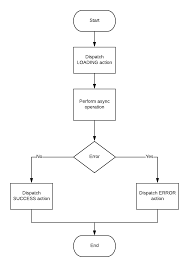
\includegraphics[scale=0.8]{figures/redux-thunk.png}
    \caption{Υλοποίηση λογικής του \tl{Redux Thunk Middleware}.}
    \label{thunk}
\end{figure}

Στην εφαρμογή, η προαναφερθείσα ροή υλοποιείται σε ενέργειες που απαιτούν τη λήψη δεδομένων από τη βάση πρωτού πυροδοτήσουν μια ενέργεια. Για παράδειγμα, όταν ο χρήστης πραγματοποιεί σύνδεση στην εφαρμογή, πυροδοτείται μια ενέργεια σύνδεσης χρήστη. Για την επιτυχή ολοκλήρωση της ενέργειας σύνδεσης θα πρέπει να γίνει λήψη των διαπιστευτηρίων του χρήστη για να διασταυρωθούν με αυτά που έδωσε ως είσοδο κατά τη διαδικασία σύνδεσης στην εφαρμογή. Έτσι, η ενέργεια σύνδεσης διακόπτεται μέχρις ότου ολοκληρωθεί το αίτημα λήψης των διαπιστευτηρίων του χρήστη από τη βάση δεδομένων. Έπειτα, η ενέργεια αποστέλλεται στον αντίστοιχο \tl{reducer} και η διαδικασία συνεχίζεται κανονικά. Στο παραπάνω παράδειγμα, η λογική που αφορά στη λήψη των διαπιστευτηρίων του χρήστη από τη βάση, αποτελεί το \tl{middleware} που εκτελείται στο ενδιάμεσο της ενέργειας σύνδεσης χρήστη στην εφαρμογή.



\subsection{Βιβλιοθήκες και Βοηθητικά Προγραμματιστικά Πακέτα}
Για την εγκατάσταση πρόσθετων βιβλιοθηκών έγινε χρήση των εργαλείων \tl{npm} και \tl{yarn}. Και τα δύο είναι βοηθητικά πακέτα διαχείρισης βιβλιοθηκών. Σκοπός τους είναι η εγκατάσταση βιβλιοθηκών και η σύνδεσή τους με τις απαραίτητες βιβλιοθήκες εξάρτησης (\tl{dependencies}) καθ' όλη την έκταση της εφαρμογής.
\newline
\indent
Στη συνέχεια θα γίνει μια αναφορά στις πιο αξιοσημείωτες βιβλιοθήκες που χρησιμοποιήθηκαν κατά την υλοποίηση της εφαρμογής.

\paragraph{\ttfamily{\tl{axios}}}
\paragraph{}
Η βιβλιοθήκη \ttfamily{\tl{axios}} χρησιμεύει για την δημιουργία και αποστολή ασύγχρονων αιτημάτων προς τον \tl{server}. Τα αιτήματα μπορούν να είναι της μορφής \ttfamily{\tl{GET, POST, PUT, DELETE}} και αναλόγως το είδος του αιτήματος μπορούν να συνοδεύονται ή όχι από δεδομένα \cite{[AXIOS]}. 


\paragraph{\ttfamily{\tl{native-base}}}
\paragraph{}
Η βιβλιοθήκη \ttfamily{\tl{native-base}} χρησιμοποιήθηκε ως επί το πλείστον για τη σχεδίαση των διεπιφανειών χρήστη της εφαρμογής. Διαδραστικά στοιχεία όπως φόρμες, πλήκτρα κλπ. έχουν σχεδιαστεί με τη βοήθεια της βιβλιοθήκης αυτής. Το χαρακτηριστικό της \ttfamily{\tl{native-base}} που την καθιστά ιδιαίτερα εξυπηρετική είναι το γεγονός ότι προσφέρει στον προγραμματιστή έτοιμα στοιχεία, τα οποία είναι ευέλικτα και πλήρως λειτουργικά. Έτσι μειώνεται σημαντικά ο απαιτούμενος χρόνος σχεδίασης και ο προγραμματιστής μπορεί να επικεντρωθεί στην υλοποίηση της λογικής της εφαρμογής \cite{[NB]}.


\paragraph{\ttfamily{\tl{react-native-router-flux}}}
\paragraph{}
Η υλοποίηση του μενού πλοήγησης εντός της εφαρμιογής έγινε με τη βοήθεια της βιβλιοθήκης \ttfamily{\tl{react-native-router-flux}}. Σύμφωνα με αυτή, κάθε οθόνη αποτελεί ένα \tl{scene} και πολλά \tl{scenes} μαζί συνιστούν ένα \tl{stack}. Κάθε \tl{scene} φέρει ιδιότητες όπως επικεφαλίδα, τίτλο, πλήκτρα πλοήγησης κλπ. Όσα \tl{scenes} βρίσκονται ομαδοποιημένα υπό ένα \tl{stack} μπορούν να διαδέχονται η μία την άλλη χάρη στην ιδιότητα μνήμης που παρέχεται στην στοίβα. Όλες οι οθόνες βρίσκονται κάτω από έναν κεντρικό δρομολογητή (\tl{router}) \cite{[RNRF]}.


\paragraph{\ttfamily{\tl{react-native-maps}}}
\paragraph{}
Η βασική βιβλιογραφία του \tl{facebook} σχετικά με τη \tl{react native} προσφέρει αυτή τη βιβλιοθήκη για την υλοποίηση διεπαφών χάρτη ως μιας καλύτερης εναλλακτικής έναντι των έτοιμων διεπαφών που υπάρχουν υλοποιημένες. Η \ttfamily{\tl{react-native-maps}} παρέχει στον προγραμματιστή μια σειρά από δυνατότητες που αφορούν στην διαμόρφωση διεπαφών χάρτη με μεγαλύτερη ευελιξία ως προς τον έλεγχο γεγονότων επάνω στο χάρτη, την μορφοποίηση της διεπιφάνειας χάρτη, την καταγραφή συντεταγμένων διαφόρων σημείων, την προγραμματισμένη μεταβολή θέσης, την χρήση διεπαφών με διαδραστικά στοιχεία και πολλά άλλα \cite{RNM}.



\subsection{Ιεράρχηση Αρχείων και Δομή Φακέλων}
Η ιεραρχία που ακολουθούν τα αρχεία δείχνει την πορεία για την κατάστρωση του σχεδίου της εφαρμογής. Υπάρχει χαρακτηριστική αντιστοιχία μεταξύ της δομής των φακέλων και της δομής της εφαρμογής. Κάθε οθόνη υλοποιείται σε ξεχωριστό φάκελο, ο οποίος περιλαμβάνει το αρχείο στο οποίο βρίσκεται ο σκελετός της συγκεκριμένης οθόνης, αλλά και τα υπόλοιπα στοιχεία που συνιστούν τα βοηθητικά \tl{components} της οθόνης. Η ονομασία των αρχείων ακολουθεί μία σύμβαση κατά την οποία τα αρχεία που περιέχουν \tl{components} ξεκινούν με κεφαλαία, ενώ οποιοδήποτε άλλο αρχείο ξεκινάει με μικρά. Αρχεία τα οποία αποτελούνται από περισσότερες από μια λέξεις ακολουθούν \tl{camelCase} γραφή (βλ. Σχ. \ref{screens}).

\begin{figure}[H]
    \centering
    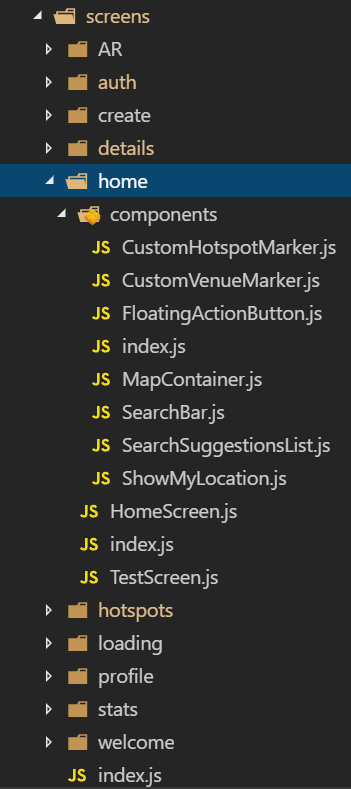
\includegraphics[scale=0.7]{figures/screens.png}
    \caption{Δομή φακέλων και αρχείων για τις οθόνες της εφαρμογής.}
    \label{screens}
\end{figure}

Η λογική που αφορά την \tl{react redux} βρίσκεται σε ξεχωριστούς φακέλους. Οι ενέργειες που πυροδοτούνται από την αλληλεπίδραση του χρήστη με τις διεπιφάνειες της εφαρμογής είναι συγκεντρωμένες στο φάκελο \tl{actions}. Κάθε \tl{action} κατατάσσεται σε διαφορετικό αρχείο, ανάλογα με το είδος του. Για παράδειγμα, \tl{actions} που αφορούν \tl{hotspots} ομαδοποιούνται σε ένα αρχείο υπό το όνομα \tl{hotspot.actions.js}. Η ίδια λογική ακολουθείται και για τα αρχεία που περιέχουν τους \tl{reducers} (βλ. Σχ. \ref{redux}).

\begin{figure}[H]
    \centering
    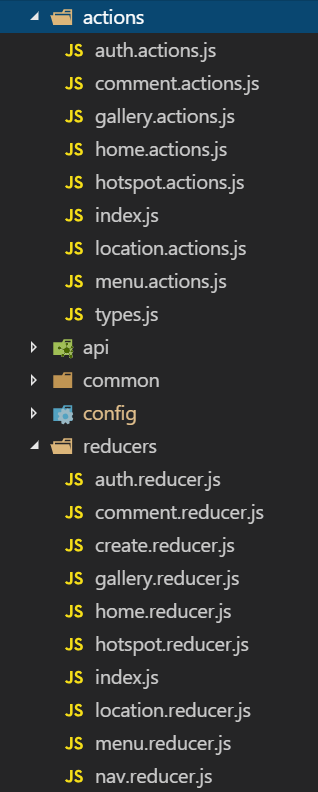
\includegraphics[scale=0.7]{figures/redux.png}
    \caption{Δομή φακέλων και αρχείων που αφορούν \tl{react redux}.}
    \label{redux}
\end{figure}

Τα αρχεία που σχετίζονται με την πλοήγηση εντός της εφαρμογής βρίσκονται σε έναν ξεχωριστό φάκελο με το όνομα \tl{routes}. Στο αρχείο με όνομα \tl{Navigator.js} βρίσκεται η υλοποίηση του κεντρικού δρομολογητή της εφαρμογής.



\section{Υλοποίηση Εξυπηρετητή Αιτημάτων και Βάσης Δεδομένων}
Σε αυτή την ενότητα θα γίνει ανάλυση των τεχνικών που εφαρμόστηκαν στην υλοποίηση του \tl{server} της εφαρμογής. Θα γίνει αναφορά στους δρομολογητές και τα αντίστοιχα \tl{routes}, καθώς και στους ελεγκτές που σχετίζονται με κάθε δρομολογητή. Θα παρουσιαστούν επίσης τα \tl{endpoints} της εφαρμογής και θα επεξηγηθούν οι λειτουργίες που αντιστοιχούν σε καθένα από αυτά.



\subsection{\tl{Server Routes}}

Ο \tl{server} χρησιμοποιεί ένα σύστημα δρομολόγησης (\tl{routes}) των αιτημάτων του \tl{client} που προορίζονται προς εξυπηρέτηση. Κάθε ομάδα υπηρεσιών που απευθύνονται σε μια συγκεκριμένη λειτουργία της εφαρμογής αντιστοιχίζεται σε ένα δρομολογητή (\tl{router}). Ο \tl{router} απαρτίζεται από επιμέρους \tl{routes}, καθεμία εκ των οποίων εξυπηρετεί μια συγκεκριμένη λειτουργία. Έτσι, στο παραπάνω παράδειγμα, το αίτημα για τη δημιουργία νέου \tl{hotspot} θα δρομολογηθεί για εξυπηρέτηση από τον \tl{router} που είναι υπεύθυνος για τις ενέργειες΄που αφορούν ένα \tl{hotspot} (\tl{\textit{HotspotRoutes}}). 

Το σύστημα των δρομολογητών έχει σχεδιαστεί με στόχο την απλότητα και την αμεσότητα στην κατανόηση από τον προγραμματιστή (βλ. Σχ. \ref{routes}). Αιτήματα που αφορούν τους χρήστες δρομολογούνται προς εξυπηρέτηση από τον \tl{router} που είναι υπεύθυνος για τις ενέργειες που αφορούν τους χρήστες. Με τον ίδιο τρόπο, Αιτήματα που σχετίζονται με σχόλια χρηστών σε ένα \tl{hotspot}, εξυπηρετούνται από εκείνο τον \tl{router} που είναι υπεύθυνος για τα σχόλια. 

\begin{figure}[h]
    \centering
    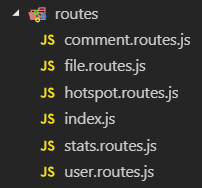
\includegraphics[scale=1]{figures/routes.png}
    \caption{Ιεράρχηση του συστήματος δρομολογητών στην εφαρμογή.}
    \label{routes}
\end{figure}

Οι δρομολογητές του συστήματος είναι οι ακόλουθοι:

\begin{itemize}
    \item \tl{\textbf{Hotspot Routes -}} περιλαμβάνει \tl{routes} που αφορούν την εξυπηρέτηση αιτημάτων σχετικά με \tl{hotspots}, όπως δημιουργία, επεξεργασία, διαγραφή, προβολή, ανάκτηση κλπ.
    \item \tl{\textbf{User Routes -}} περιλαμβάνει \tl{routes} που αφορούν την εξυπηρέτηση αιτημάτων σχετικά με χρήστες, όπως εγγραφή, σύνδεση, επεξεργασία, προβολή, ανάκτηση κλπ.
    \item \tl{\textbf{Comment Routes -}} περιλαμβάνει \tl{routes} που αφορούν την εξυπηρέτηση αιτημάτων σχετικά με σχόλια, όπως δημιουργία, προβολή, απαρίθμηση κλπ.
    \item \tl{\textbf{File Routes -}} περιλαμβάνει \tl{routes} που αφορούν την εξυπηρέτηση αιτημάτων σχετικά με συνημμένα αρχεία σε \tl{hotspots}.
    \item \tl{\textbf{Stats Routes -}} περιλαμβάνει \tl{routes} που αφορούν την εξυπηρέτηση αιτημάτων σχετικά με στατιστικά δεδομένα.
\end{itemize}

\subsection{\tl{Server Controllers}}

Αφότου τα αιτήματα δρομολογηθούν προς εξυπηρέτηση στους αντίστοιχους \tl{routers}, ακολοθεί η επεξεργασία τους και η εκτέλεσή τους μέσω κατάλληλων μεθόδων. Οι μέθοδοι που αναλαμβάνουν την εκτέλεση των αιτημάτων ονομάζονται ελεγκτές (\tl{controllers}) και αποτελούνται από ένα σύνολο ασύγχρονων εντολών και κλήσεων μεταξύ της βάσης δεδομένων και του \tl{server}.

Όπως και με το σύστημα των δρομολογητών, έτσι και οι ελεγκτές έχουν σχεδιαστεί με στόχο να αποσυμπλέκουν τις ενέργειες που σχετίζονται με κάθε αίτημα (βλ. Σχ. \ref{controllers}). Όλες οι ενέργεεις που αφορούν τα \tl{hotspots} εκτελούνται αποκλειστικά από έναν ελεγκτή. Το ίδιο συμβαίνει και με τις ενέργεεις γύρω από τους χρήστες. Το σύστημα των \tl{controllers} έχει παραπλήσια μορφή με αυτό των \tl{routers} καθώς στόχος της σχεδίασης είναι να υπάρχει ένας βαθμός αναλογίας μεταξύ των διαφόρων τμημάτων,ο οποίος μειώνει αισθητά το χρόνο κατανόησης και βελτιστοποιεί τη διαδικασία υλοποίησης:

\begin{itemize}
    \item \tl{\textbf{Hotspot Controller -}} περιλαμβάνει τις μεθόδους που αφορούν την εξυπηρέτηση αιτημάτων σχετικά με \tl{hotspots}, όπως δημιουργία, επεξεργασία, διαγραφή, προβολή, ανάκτηση κλπ.
    \item \tl{\textbf{User Controller -}} περιλαμβάνει τις μεθόδους που αφορούν την εξυπηρέτηση αιτημάτων σχετικά με χρήστες, όπως εγγραφή, σύνδεση, επεξεργασία, προβολή, ανάκτηση κλπ.
    \item \tl{\textbf{Comment Controller -}} περιλαμβάνει τις μεθόδους που αφορούν την εξυπηρέτηση αιτημάτων σχετικά με σχόλια, όπως δημιουργία, προβολή, απαρίθμηση κλπ.
    \item \tl{\textbf{File Controller -}} περιλαμβάνει τις μεθόδους που αφορούν την εξυπηρέτηση αιτημάτων σχετικά με συνημμένα αρχεία σε \tl{hotspots}.
    \item \tl{\textbf{Stats Controller -}} περιλαμβάνει τις μεθόδους που αφορούν την εξυπηρέτηση αιτημάτων σχετικά με στατιστικά δεδομένα.
    \item \tl{\textbf{Views Controller -}} περιλαμβάνει τις μεθόδους που αφορούν την εξυπηρέτηση αιτημάτων σχετικά με τα \tl{views} ενός \tl{hotspot}.
\end{itemize}

\begin{figure}[h]
    \centering
    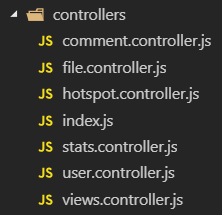
\includegraphics[scale=1]{figures/controllers-path-vscode.png}
    \caption{Ιεράρχηση του συστήματος ελεγκτών στην εφαρμογή.}
    \label{controllers}
\end{figure}

\subsection{\tl{REST API - Server Endpoints}}
Κάθε ενέργεια από την πλευρά του \tl{client} πυροδοτεί ένα αίτημα στην πλευρά του \tl{server}. Στην ενότητα αυτή αναλύεται η τεχνική με την οποία ταξινομούνται και δρομολογούνται τα αιτήματα σε συγκεκριμένα \tl{endpoints}.


\begin{itemize}
    \item \tl{hotspots}
    \newline \newline
    \textbf{\tl{\ttfamily{GET /hotspots/radius?lat=''&lng=''}}}
    \newline \newline
    \textbf{-\tl{lat}} - συντεταγμένη γεωγραφικού πλάτους (\tl{latitude}) \newline 
    \indent
    \textbf{-\tl{lng}} - συντεταγμένη γεωγραφικού μήκους (\tl{longitude})
    \newline \newline \noindent
    ανακτά όλα τα μηνύματα εντός της προκαθορισμένης ακτίνας των 5000 μέτρων από τη δεδομένη θέση που καθορίζεται από το γεωγραφικό πλάτος (\tl{lat}) και το γεωγραφικό μήκος (\tl{lng}).
    
    \newline \newline
    \textbf{\tl{\ttfamily{GET /hotspots/:hospotId}}}
    \newline \newline \noindent
    ανακτά τις πληροφορίες που αφορούν το μηνύμα με το συγκεκριμένο αναγνωριστικό \tl{hotspotId}.
    
    \newline \newline
    \textbf{\tl{\ttfamily{GET /users/:userId/hotspots}}}
    \newline \newline \noindent
    ανακτά όλα τα μηνύματα του χρήστη με το συγκεκριμένο αναγνωριστικό \tl{userId}.
    
    \newline \newline
    \textbf{\tl{\ttfamily{POST /hotspots/new}}}
    \newline \newline \noindent
    δημιουργεί μια νέα είσοδο για την αποθήκευση ενός καινούριου \tl{hotspot} στη βάση.
    
    \newline \newline
    \textbf{\tl{\ttfamily{PUT /hotspots/:hotspotId/edit}}}
    \newline \newline \noindent
    επεξεργάζεται το \tl{hotspot} με το προκαθορισμένο αναγνωριστικό \tl{hotspotId}, με τα δοθέντα στοιχεία.
    
    \newline \newline
    \textbf{\tl{\ttfamily{DELETE /hotspots/:hotspotId/delete}}}
    \newline \newline \noindent
    διαγράφει το \tl{hotspot} με το προκαθορισμένο αναγνωριστικό \tl{hotspotId} από τη βάση δεδομένων.
    
    \item \tl{users}
    
    \newline \newline
    \textbf{\tl{\ttfamily{GET /users/:userId}}}
    \newline \newline \noindent
    ανακτά τα στοιχεία του χρήστη που προσδιορίζεται από το αναγνωριστικό \tl{userId}.
    
    \newline \newline
    \textbf{\tl{\ttfamily{POST /register}}}
    \newline \newline \noindent
    πραγματοποιεί εγγραφή ενός νέου χρήστη στο σύστημα, τα αποθηκεύει τα στοιχεία στη βάση και εκδίδει σύμβολο ταυτοποίησης (\tl{access token}).
    
    \newpage
    \newline \newline
    \textbf{\tl{\ttfamily{POST /login}}}
    \newline \newline \noindent
    πραγματοποιεί σύνδεση ενός χρήστη στην εφαρμογή και εκδίδει σύμβολο ταυτοποίησης (\tl{access token}).
    
    \newline \newline
    \textbf{\tl{\ttfamily{POST /verify}}}
    \newline \newline \noindent
    πραγματοποιεί έλεγχο της ταυτότητας του χρήστη διασταυρώνοντας το σύμβολο ταυτοποίησης του χρήστη με αυτό που είναι αποθηκευμένο στη βάση.
    
    \newline \newline
    \textbf{\tl{\ttfamily{PUT /users/:userId/edit}}}
    \newline \newline \noindent
    επεξεργάζεται τα στοιχεία του χρήστη που καθορίζεται από το αναγνωριστικό \tl{userId} και αποθηκεύει τον ανανεωμένο χρήστη στη βάση.
    
    \item \tl{comments}
    
    \newline \newline
    \textbf{\tl{\ttfamily{GET /:userId/hotspots/:hotspotId/comments}}}
    \newline \newline \noindent
    ανακτά τα σχόλια ενός \tl{hotspot} με τη βοήθεια των διακριτικών \tl{hotspotId} και \tl{userId}.
    
    \newline \newline
    \textbf{\tl{\ttfamily{POST /:userId/hotspots/:hotspotId/comments/new}}}
    \newline \newline \noindent
    δημιουργεί μια είσοδο στη βάση για την αποθήκευση ενός καινούριου σχολίου. Χρειάζεται το αναγνωριστικό του \tl{hotspot} στο οποίο έγινε το σχόλιο, καθώς επίσης και του διακριτικού του χρήστη που έκανε το σχόλιο.
    
    \item \tl{files}
    
    \newline \newline
    \textbf{\tl{\ttfamily{GET /users/:userId/gallery}}}
    \newline \newline \noindent
    ανακτά όλα τα αρχεία ενός χρήστη με το συγκεκριμένο αναγνωριστικό \tl{userId}.
    
    \newline \newline
    \textbf{\tl{\ttfamily{POST /users/:userId/gallery/upload}}}
    \newline \newline \noindent
    δημιουργεί μια νέα είσοδο στη βάση για την αποθήκευση ενός αρχείου που αφορά το χρήστη με το συγκεκριμένο αναγνωριστικό \tl{userId}.
    
    \newline \newline
    \textbf{\tl{\ttfamily{DELETE /gallery/:fileId/delete}}}
    \newline \newline \noindent
    διαγράφει το αρχείο με το προκαθορισμένο αναγνωριστικό \tl{fileId} από τη βάση δεδομένων όταν διαγραφεί ένα \tl{hotspot}.
    
    \item \tl{stats}
    
    \newline \newline
    \textbf{\tl{\ttfamily{GET /stats/users}}}
    \newline \newline \noindent
    ανακτά το συνολικό αριθμό των χρηστών που χρησιμοποιούν την εφαρμογή.
    
    \newline \newline
    \textbf{\tl{\ttfamily{GET /stats/comments}}}
    \newline \newline \noindent
    ανακτά το συνολικό αριθμό των σχολίων που έχουν δημιουργηθεί εντός της εφαρμογής.
    
    \newline \newline
    \textbf{\tl{\ttfamily{GET /stats/hotspots}}}
    \newline \newline \noindent
    ανακτά το συνολικό αριθμό των \tl{hotspots} που έχουν δημιουργηθεί εντός της εφαρμογής.
    
    \newline \newline
    \textbf{\tl{\ttfamily{GET /stats/views}}}
    \newline \newline \noindent
    ανακτά το συνολικό αριθμό των \tl{views} που έχουν δημιουργηθεί εντός της εφαρμογής.
    
    \newline \newline
    \textbf{\tl{\ttfamily{GET /stats/:userId/hotspots}}}
    \newline \newline \noindent
    ανακτά το συνολικό αριθμό των \tl{hotspots} που έχουν δημιουργηθεί από τον χρήστη με το συγκεκριμένο αναγνωριστικό \tl{userId}.
    
    \newline \newline
    \textbf{\tl{\ttfamily{GET /stats/:userId/comments}}}
    \newline \newline \noindent
    ανακτά το συνολικό αριθμό των σχολίων που έχουν δημιουργηθεί από τον χρήστη με το συγκεκριμένο αναγνωριστικό \tl{userId}.
    
    \newline \newline
    \textbf{\tl{\ttfamily{GET /stats/:userId/ratio}}}
    \newline \newline \noindent
    ανακτά το ποσοστό αγοριών/κοριτσιών που έχουν προβάλλει τα \tl{hotspots} του χρήστη με το συγκεκριμένο αναγνωριστικό \tl{userId}.
    
   
\end{itemize}

\subsubsection{Βιβλιοθήκες και Βοηθητικά Προγραμματιστικά Πακέτα}
Για την εγκατάσταση πρόσθετων βιβλιοθηκών έγινε και εδώ χρήση των εργαλείων \tl{npm} και \tl{yarn}. Στη συνέχεια θα γίνει μια αναφορά στις πιο αξιοσημείωτες βιβλιοθήκες που χρησιμοποιήθηκαν κατά την υλοποίηση του εξυπηρετητή και της βάσης δεδομένων.

\paragraph{\ttfamily{\tl{passport}}}
\paragraph{}
Η βιβλιοθήκη \ttfamily{\tl{passport}} αποτελεί ένα είδος \tl{middleware} για την ταυτοποίηση χρηστών. Χρησιμοποιώντας τεχνικές ταυτοποίησης που ονομάζονται \tl{strategies}, καθορίζει τον τρόπο με τον οποίο γίνεται η ταυτοποίηση χρηστών στα διάφορα σενάρια που περιλαμβάνει η εφαρμογή \cite{[PASSPORT]}. 


\paragraph{\ttfamily{\tl{babel}}}
\paragraph{}
Η βιβλιοθήκη \ttfamily{\tl{babel}} χρησιμοποιήθηκε ως ο βασικός μεταγλωττιστής του κώδικα από \tl{ES6} σε \tl{ES5}. Η \ttfamily{\tl{babel}} υποστηρίζει την πιο πρόσφατη έκδοση \tl{JavaScript} χρησιμοποιώντας συντακτικούς μετατροπείς (\tl{syntax transformers}) \cite{[BABEL]}.


\paragraph{\ttfamily{\tl{mongoose}}}
\paragraph{}
Η βιβλιοθήκη \ttfamily{\tl{mongoose}} χρησιμοποιήθηκε για την προσθήκη κάποιων βασικών ιδιοτήτων στην βάση δεδομένων. Τέτοιες είναι η μοντελοποίηση της βάσης σε \tl{models} με συγκεκριμένη δομή. Εξίσου σημαντική είναι η δυνατότητα σελιδοποίησης των \tl{collections} εντός της βάσης και η επιστροφή σελιδοποιημένων αποτελεσμάτων σε κάθε αναζήτηση \cite{[MONGOOSE]}. 


\paragraph{\ttfamily{\tl{bcryptjs}}}
\paragraph{}
Η βιβλιοθήκη \ttfamily{\tl{bcryptjs}} χρησιμοποιείται για την κρυπτογράφηση ευαίσθητων πληροφοριών που αποθηκεύονται στη βάση δεδομένων. Συνήθως χρησιμεύει για την κρυπτογράφηση κωδικών πρόσβασης και την αποφυγή κατάχρησής τους από κακόβουλο λογισμικό \cite{[BCRYPT]}.





\section{\tl{Expo SDK \& Expo Client}}
Η ανάπτυξη \tl{iOS} εφαρμογών γίνεται μόνο στις αντίστοιχες \tl{iOS} πλατφόρμες. Για την υλοποίηση εφαρμογών σε άλλες πλατφόρμες (πχ. \tl{Windows}) είναι απαραίτητη η χρήση ενός ενδιάμεσου λογισμικού για την φιλοξενία της εφαρμογής. Το \tl{Expo} είναι διαμορφωμένο ώστε να διευκολύνει τον προγραμματιστή με τον ταυτοχρονισμό της ανάπτυξης εφαρμογών και ελέγχου λειτουργίας.
\newline
\indent
Το \tl{Expo SDK} παρέχει στον προγραμματιστή όλες τις μητρικές διεπαφές που διατίθενται στις μητρικές γλώσσες προγραμματισμού. Τα βασικά \tl{APIs} όπως η κάμερα, οι ειδοποιήσεις, η τοποθεσία, η συλλογή φωτογραφιών κλπ. μπορούν να χρησιμοποιηθούν άμεσα, χωρίς πρόσθετη λογική, όπως θα γινόταν στον προγραμματισμό σε \tl{Swift}. Στόχος του λογισμικού είναι να εξομαλύνει όσο το δυνατό περισσότερο την εμπειρία προγραμματισμού, αλλά και την εμπειρία χρήσης των διεπιφανειών, μειώνοντας τις διαφορές στο ελάχιστο. Η πλατφόρμα προσπαθεί να καλύπτει όλα τα δυνατά σενάρια χρήσης που εμφανίζονται στις σύγχρονες εφαρμογές, καθιστώντας των κώδικα πλήρως δυναμικό.
\newline
\indent
Με την εγκατάσταση του \tl{Expo Client} σε μια συσκευή \tl{iOS} ο προγραμματιστής μπορεί να πραγματοποιεί έλεγχο σε πραγματικό χρόνο. Ο \tl{Expo Client} φιλοξενεί την υπό ανάπτυξη εφαρμογή σε ένα περιβάλλον ειδικά διαμορφωμένο για αυτό τον σκοπό. Κατά τον έλεγχο της εφαρμογής, εμφανίζονται ειδικά μηνύματα σφάλματος στον προγραμματιστή που βοηθάνε στη διαδιακσία αποσφαλμάτωσης της εφαρμογής σε πραγματικό χρόνο. Έτσι, μειώνεται σε μεγάλο βαθμό η δυσκολία εύρεσης σφαλμάτων στον κώδικα, καθώς και ο χρόνος αποσφαλμάτωσης της εφαρμογής.


\section{\tl{Visual Studio Code}}

Η πλατφόρμα προγραμματισμού που προτιμήθηκε στην ανάπτυξη της εφαρμογής ήταν το \tl{VSCode} της \tl{\textit{Microsoft}}. Η επιλογή βασίστηκε στις αμέτρητες δυνατότητες που προσφέρει η πλατφορμα αυτή. Σημαντικοί παράγοντες αποτέλεσαν επίσης η ευελιξία στον τρόπο προγραμματισμού, η αυξημένη ελαστικότητα ως προς τη διαμόρφωση του περιβάλλοντος προγραμματισμού εντός της πλατφόρμας, καθώς επίσης και η μεγάλη υποστήριξη που λαμβάνει η πλατφόρμα από την παγκόσμια προγραμματιστική κοινότητα.

<<<<<<< HEAD
\chapter{Έλεγχος}
\label{chap6}
=======
\chapter{Τεχνικές λεπτομέρειες}
\label{chap7}
>>>>>>> acacc83a12cc6f1be99d6d3fb0df8b0ed3fa708b

Εδώ λέμε ότι θα ακολουθήσουν τεχνικές λεπτομέρειες της διπλωματικής.

\section{Λεπτομέρειες υλοποίησης}

Εδώ περιγράφουμε λεπτομερώς θέματα της διπλωματικής που έχουν τεχνικό ενδιαφέρον. Προσδιορίστε επομένως τα θέματα αυτά, βάλτε μια ενότητα για κάθε ένα και περιγράψτε τα αναλυτικά. Η περιγραφή μπορεί να γίνει βάζοντας κομμάτια κώδικα ή ψευδοκώδικα, και περιγράφοντάς τα με λόγια. Μην ξεχνάτε να δίνετε πάντα παραδείγματα για το πώς τρέχει ένα κομμάτι κώδικα π.χ. για έναν αλγόριθμο.

\subsection{<Τίτλος θέματος 1>}
Γράψτε το κείμενό σας εδώ ...

\subsection{<Τίτλος θέματος 1>}
Γράψτε το κείμενό σας εδώ ...

\section{Πλατφόρμες και προγραμματιστικά εργαλεία}

Εδώ περιγράφονται τα χαρακτηριστικά της συγκεκριμένης υλοποίησης, όπως η πλατφόρμα ανάπτυξης και εκτέλεσης, τα προγραμματιστικά εργαλεία, οι απαιτήσεις της εφαρμογής σε hardware, κ.λ.π. Επίσης, περιγράφεται λεπτομερώς η διαδικασία εγκατάστασης της διπλωματικής σε υπολογιστή. Προσέξτε να δίνονται όλες οι λεπτομέρειες, το απαραίτητο λογισμικό και οι αναγκαίες ρυθμίσεις.

\chapter{Επίλογος}
\label{chap8}

Εδώ εξηγούμε ότι θα συνοψίσουμε την μελέτη που εκπονήθηκε στα πλαίσια της διπλωματικής.

\section{Σύνοψη και συμπεράσματα}

Εδώ συνοψίζουμε τα αποτελέσματα της διπλωματικής και περιγράφουμε τα συμπεράσματα που προέκυψαν, αρνητικά και θετικά. Επιβεβαιώνουμε την συνεισφορά της διπλωματικής στα προβλήματα που αναφέραμε στην εισαγωγή.

\section{Μελλοντικές επεκτάσεις}

Εδώ δίνουμε ιδέες για επέκταση της διπλωματικής.




%OPTION #1: Embed bibliography from file `references.tex' using plain references.

\begin{thebibliography}{1}

\addcontentsline{toc}{chapter}{Βιβλιογραφία}

\bibitem{[AMP+14]} {\textlatin{
{Jeff Sondermann, {\em American Press Institute}}.
Mobile and social media are intricately linked.
\url{https://www.americanpressinstitute.org/publications/reports/white-papers/mobile-and-social-media/ }
  2014. Last accessed on 07/03/2019}}.
  
\bibitem{[VEN+18]} {\textlatin{
{Ricardo Bilton}.
New data shows just how much social sharing has decreased since 2015 (and News Feed tweaks are just one factor).
\url{https://www.venturelean.team/hello-world/ }
  2018. Last accessed on 08/03/2019}}.
  
\bibitem{[BBC+18]} {\textlatin{
{Jessica Brown, {\em BBC Future}}.
Is social media bad for you? The evidence and the unknowns.
\url{http://www.bbc.com/future/story/20180104-is-social-media-bad-for-you-the-evidence-and-the-unknowns }
  2018. Last accessed on 08/03/2019}}.

\bibitem{[CSW+18]} {\textlatin{
{CrowdSourcingWeek}.
What is Crowdsourcing?
\url{https://crowdsourcingweek.com/what-is-crowdsourcing/ }
  2018. Last accessed on 08/03/2019}}.
  
\bibitem{[WIT+18]} {\textlatin{
{ISLAB Team, NTUA}.
About WITH
\url{http://withcrowd.eu/about }
  2018. Last accessed on 08/03/2019}}.
 
\bibitem{[4SQ+18]} {\textlatin{
{Foursquare Developer Team}.
Foursquare API
\url{https://developer.foursquare.com/docs/api/endpoints }
  2018. Last accessed on 08/03/2019}}.
  
\bibitem{[IND+16]} {\textlatin{
{Grace Fearon, {\em iStudent}}.
Our need to maintain social approval is actually making us lose what is best about ourselves - our individuality.
\url{https://www.independent.co.uk/student/istudents/our-need-to-maintain-social-approval-is-actually-making-us-lose-what-is-best-about-ourselves-our-a6827316.html }
   2016. Last accessed on 08/03/2019}}.
  
\bibitem{[JAR+18]} {\textlatin{
{Mansi Beniwal}.
Social Media and its Impact in Interpersonal Relationships.
\url{https://jarvee.com/social-media-impact-interpersonal-relationships/ }
  2018. Last accessed on 08/03/2019}}.
  
\bibitem{[SQA+07]} {\textlatin{
{Ullah, Asmat}.
Client Side Scripting for Web Applications
\url{https://www.sqa.org.uk/e-learning/SiteHomeCD/page_26.htm }
  2007. Last accessed on 08/03/2019}}.
  
\bibitem{[STR+09]} {\textlatin{
{Stroustrup, Bjarne}.
Bjarne Stroustrup's FAQ: What do you think of C++/CLI?
\url{http://www.stroustrup.com/bs_faq.html#CppCLI}
  2009. Last accessed on 08/03/2019}}.
  
\bibitem{[DEV+03]} {\textlatin{
{Gregory, Kate}.
Managed, Unmanaged, Native: What Kind of Code Is This?
\url{https://www.developer.com/net/cplus/article.php/2197621 }
  2003. Last accessed on 08/03/2019}}.
  
\bibitem{[MIC05]} {\textlatin{
Meijer, Erik and Peter Drayton. Static Typing Where Possible, Dynamic Typing When Needed: The End of the Cold War Between Programming Languages. Microsoft Corporation, 2005. Last accessed on 08/03/2019}}.  

\bibitem{[ADV09]} {\textlatin{
L.~Tratt. Dynamically Typed Languages. {\em Advances in Computers}, 77(2):149--184, July 2009. Last accessed on 08/03/2019}}.  
 
\bibitem{[SWIFT1+16]} {\textlatin{
{Apple Inc., {\em swift.org}}.
The Swift Linux Port
\url{https://swift.org/blog/swift-linux-port/}
  2016. Last accessed on 10/03/2019}}.
  
\bibitem{[SWIFT2+14]} {\textlatin{
{Chris Lattner}.
Chris Lattner's Homepage
\url{http://nondot.org/sabre/}
  2014. Last accessed on 10/03/2019}}.
  
\bibitem{[SWIFT3+14]} {\textlatin{
{Apple Worldwide Developers Conference, Session 102}.
Platforms State of the Union
  2016. Last accessed on 10/03/2019}}.

\bibitem{[SWIFT4]} {\textlatin{
{ Rachel Metz, {\em MIT Technology}}.
Apple Seeks a Swift Way to Lure More Developers
\url{https://www.technologyreview.com/s/527821/apple-seeks-a-swift-way-to-lure-more-developers/}
  2014. Last accessed on 10/03/2019}}.
  
\bibitem{[SWIFT5]} {\textlatin{
{Harrison Weber, {\em VentureBeat}}.
Apple announces 'Swift', a new programming language for macOS & iOS
\url{https://venturebeat.com/2014/06/02/apple-introduces-a-new-programming-language-swift-objective-c-without-the-c/}
  2014. Last accessed on 10/03/2019}}.

\bibitem{[JAVA1]} {\textlatin{
{J.~Gosling, J.~Bill, G.~Steele, G.~Bracha, A.~Buckley}.
The Java® Language Specification
{\em Java SE 8th edition}, 2014. Last accessed on 11/03/2019}}.

\bibitem{[JAVA2]} {\textlatin{
{Computer Weekly}.
Write once, run anywhere?
\url{http://www.computerweekly.com/Articles/2002/05/02/186793/write-once-run-anywhere.htm}
  2002. Last accessed on 11/03/2019}}.
  
\bibitem{[JAVA3]} {\textlatin{
{Oracle Inc.}.
Design Goals of the Java™ Programming Language
\url{https://www.oracle.com/technetwork/java/intro-141325.html}
  2013. Last accessed on 11/03/2019 }}.
  
\bibitem{[JAVA4]} {\textlatin{
{R.~McMillan, {\em wired.com}}.
Is Java Losing Its Mojo?
\url{https://www.wired.com/2013/01/java-no-longer-a-favorite/}
  2013. Last accessed on 11/03/2019}}.
  
\bibitem{[JAVA5]} {\textlatin{
{Stephen O'Grady, {\em RedMonk}}.
The RedMonk Programming Language Rankings: January 2015
\url{https://redmonk.com/sogrady/2015/01/14/language-rankings-1-15/}
  2015. Last accessed on 11/03/2019}}.
  
\bibitem{[JAVA6]} {\textlatin{
{{\em langpop.com}}.
Programming Language Popularity
\url{https://web.archive.org/web/20090116080326/http://www.langpop.com/}
  2009. Last accessed on 11/03/2019}}.
  
\bibitem{[JAVA7]} {\textlatin{
{Tata McGraw}. 
Object-oriented Programming with Java: Essentials and Applications.
{\em Hill Education}, 1:30--35, 2009. Last accessed on 11/03/2019}}.  

\bibitem{[JAVA8]} {\textlatin{
{Sun Microsystems, {\em WaybackMachine}}.
JAVASOFT SHIPS JAVA 1.0 - {\em
Programming environment available free for developers}
\url{https://web.archive.org/web/20070310235103/http://www.sun.com/smi/Press/sunflash/1996-01/sunflash.960123.10561.xml}
  2018. Last accessed on 11/03/2019}}.  
  
\bibitem{[JAVA9]} {\textlatin{
{Alex Mullis, {\em Android Authority}}.
How to install the Android SDK (Software Development Kit)
\url{https://www.androidauthority.com/how-to-install-android-sdk-software-development-kit-21137/}
  2016. Last accessed on 11/03/2019}}. 
  
\bibitem{[JAVA10]} {\textlatin{
{Android Developers}.
Introduction to Android
\url{https://developer.android.com/guide/index.html}
  2017. Last accessed on 11/03/2019}}.  
  
\bibitem{[JAVA11]} {\textlatin{
{Android Developers}.
Tools Overview
\url{https://developer.android.com/studio/command-line/}
  2012. Last accessed on 11/03/2019}}.  
  
\bibitem{[JS1]} {\textlatin{
Stoyan Stefanov.
JavaScript Patterns.
{\em O'Reilly Media, Inc.}, 1(1): 5--10, 2010. Last accessed on 14/03/2019}}.  

\bibitem{[JS2]} {\textlatin{
{{\em w3techs.com}}.
Usage Statistics of JavaScript for Websites
\url{https://w3techs.com/technologies/details/cp-javascript/all/all}
  2015. Last accessed on 14/03/2019}}. 
  
\bibitem{[JS3]} {\textlatin{
{{\em pabbly.com}}.
NodeJS Event Loops
\url{https://www.pabbly.com/tutorials/node-js-event-loops/}}. 2015. Last accessed on 14/03/2019}. 

\bibitem{[AJAX1]} {\textlatin{
{Jesse James Garrett, {\em AdaptivePath}}.
Ajax: A New Approach to Web Applications
\url{https://adaptivepath.org/ideas/ajax-new-approach-web-applications/}
  2005. Last accessed on 14/03/2019}}.

\bibitem{[AJAX2]} {\textlatin{
{Modzilla Developer Network Web Docs, {\em MDN.com}}.
 Ajax - Web developer guides
\url{https://developer.mozilla.org/en-US/docs/Web/Guide/AJAX}
  2018. Last accessed on 14/03/2019}}.  

\bibitem{[SPA1]} {\textlatin{
David Flanagan. 
JavaScript - The Definitive Guide.
{\em O'Reilly, Sebastpool, CA}, 1(5):495--450, 2006}}.

\bibitem{[MVC1]} {\textlatin{
{Steve Burbeck}.
 Applications Programming in Smalltalk-80:How to use Model–View–Controller (MVC)
\url{https://web.archive.org/web/20120729161926/http://st-www.cs.illinois.edu/users/smarch/st-docs/mvc.html}
  1992. Last accessed on 14/03/2019}}.  

\bibitem{[REACT1]} {\textlatin{
{Facebook, {\em reactjs.org}}.
 Components and Props
\url{https://reactjs.org/docs/components-and-props.html#props-are-read-only}
  2018. Last accessed on 17/03/2019}}.  
  
\bibitem{[REACT2]} {\textlatin{
{React Blog, {\em reactjs.org}}.
 Refs and DOM
\url{https://reactjs.org/docs/refs-and-the-dom.html}
  2018. Last accessed on 17/03/2019}}.  
  
\bibitem{[REACT3]} {\textlatin{
{Facebook}.
 JSX Specification
\url{https://facebook.github.io/jsx/}
  2018. Last accessed on 17/03/2019}}. 
  
\bibitem{[REACT4]} {\textlatin{
{{\em reactjs.org}, tutorials}.
 Tutorial: intro to React
\url{https://reactjs.org/tutorial/tutorial.html}
  2017. Last accessed on 17/03/2019}}. 
  
\bibitem{[RN1]} {\textlatin{
Bonnie Eisenman. 
Learning React Native.
{\em O'Reilly Media, Inc.}, chapter 1, 2015. Last accessed on 18/03/2019}}. 

\bibitem{[RN2]} {\textlatin{
Tal Kol, {\em Wix.com}. 
Building a React Native App for 80 Million Users.
From {\em ReactNext Conference 2016, Tel Aviv},
\url{https://www.youtube.com/watch?v=abSNo2P9mMM&feature=youtu.be&t=17m34s},
minutes 17:37--33:20, 2016. Last accessed on 18/03/2019}}.

\bibitem{[RN3]} {\textlatin{
{Natalia Chrzanowska}.
 13 Great Examples of React Native Apps
\url{https://www.netguru.com/blog/13-great-apps-written-with-react-native}
  2019. Last accessed on 18/03/2019}}.
  
\bibitem{[RN4]} {\textlatin{
{Marvin Frachet, {\em hackermoon.com}}.
Understanding the React Native bridge concept
\url{https://hackernoon.com/understanding-react-native-bridge-concept-e9526066ddb8}
  2018. Last accessed on 18/03/2019}}.
  
\bibitem{[NODE1]} {\textlatin{
{Tomislav Capan, {\em toptal.com}}.
Why Use Node.js?
\url{https://www.toptal.com/nodejs/why-the-hell-would-i-use-node-js}
  2013. Last accessed on 19/03/2019}}.
  
\bibitem{[NODE2]} {\textlatin{
{Kenneth Peeples, {\em dzone.com}}.
What are the Benefits of Node.js?
\url{https://dzone.com/articles/what-are-benefits-nodejs}
  2015. Last accessed on 19/03/2019}}.
  
\bibitem{[NODE3]} {\textlatin{
{Node,js Foundation, {\em nodejs.org}}.
Node.js Docs
\url{https://nodejs:org}. Last accessed on 19/03/2019}}.
  
\bibitem{[NODE4]} {\textlatin{
{Expolarions of an Engineer, {\em timcosta.io}}.
The Node.js Event Loop
\url{https://www.timcosta.io/the-node-js-event-loop/}
  2016. Last accessed on 19/03/2019}}.

\bibitem{[REST1]} {\textlatin{
RESTful Web Services Architecture.
Of the {\em World Wide Web Consortium}, Chapter 3.1.3: Relationship to the World Wide Web and REST Architectures, February 2004. Last accessed on 19/03/2019}}.

\bibitem{[REST2]} {\textlatin{
{R.~T. Fielding}
Architectural Styles and the Design of Network-based Software Architectures (Ph.D.). { \em Chapter 5: Representational State Transfer (REST)}. University of California, Irvine. 2000. Last accessed on 19/03/2019}}.

\bibitem{[REST3]} {\textlatin{
{L.~Richardson, M.~Amundsen}
RESTful Web APIs, { \em O'Reilly Media}. 2013 {\em ISBN 978-1-449-35806-8}}}.

\bibitem{[MONGO1]} {\textlatin{
{Davis Kerby}
Why MongoDB is the Way to Go, {\em DZone}.
\url{https://dzone.com/articles/why-mongodb-is-worth-choosing-find-reasons}
  2015. Last accessed on 20/03/2019}}.

\bibitem{[MONGO2]} {\textlatin{
{{\em ClusterHQ}}.
Ridiculously fast MongoDB replica recovery Part 1 of 2
\url{http://clusterhq.com/2016/03/14/ridiculously-fast-mongodb-replica-recovery-with-flocker/}. Last accessed on 20/03/2019}}.

\bibitem{[MONGO3]} {\textlatin{
{{\em Severalnines}}.
Turning MongoDB Replica Set to a Sharded Cluster
\url{https://severalnines.com/blog/turning-mongodb-replica-set-sharded-cluster}
  2013. Last accessed on 20/03/2019}}.

\bibitem{[MONGO4]} {\textlatin{
{{\em Compose}}.
GridFS \& MongoDB: Pros And Cons
\url{https://www.compose.com/articles/gridfs-and-mongodb-pros-and-cons/}
  2014. Last accessed on 20/03/2019}}.

\bibitem{[MONGO5]} {\textlatin{
{Md.~Malick, {\em ExpertsTown}}.
MongoDB Overview
\url{https://www.hugedomains.com/domain_profile.cfm?d=expertstown&e=com}
  2013. Last accessed on 20/03/2019}}.

\bibitem{[MONGO6]} {\textlatin{
{MongoDB Docs, {\em docs.mongodb.com}}.
Aggregation — MongoDB Manual
\url{https://docs.mongodb.com/manual/aggregation/}. Last accessed on 20/03/2019}}.

\bibitem{[MONGO7]} {\textlatin{
{MongoDB Docs, {\em docs.mongodb.com}}.
Map-Reduce — MongoDB Manual
\url{https://docs.mongodb.com/manual/core/map-reduce/}. Last accessed on 20/03/2019}}.

\bibitem{[JWT1]} {\textlatin{
J.~Bradley, N.~Sakimura, M.~Jones,
JSON Web Token (JWT)
{\em  Mastering Identity and Access Management with Microsoft Azzure}, 1(1):84, ISBN: 9781785887888}}.








\bibitem{[DRS09]} {\textlatin{
N.~Dalvi, C.~R{\'e}, and D.~Suciu. Probabilistic databases: Diamonds in the dirt. {\em Communications of the ACM}, 52(7):86--94, July 2009}}.

\bibitem{[GBE+00]} {\textlatin{
R.~H. G{\"u}ting, M.~H. B{\"o}hlen, M.~Erwig, C.~S. Jensen, N.~A. Lorentzos,
  M.~Schneider, and M.~Vazirgiannis.
A foundation for representing and querying moving objects.
{\em ACM Transactions on Database Systems (TODS)}, 25(1):1--42, 2000}}.

\bibitem{[JMS+08]} {\textlatin{
N.~Jain, S.~Mishra, A.~Srinivasan, J.~Gehrke, J.~Widom, H.~Balakrishnan,
  U.~{\c{C}}etintemel, M.~Cherniack, R.~Tibbetts, and S.~Zdonik.
Towards a streaming {SQL} standard.
In {\em Proceedings of the VLDB Endowment}, 1(2):1379--1390, 2008}}.

\bibitem{[MHP05]} {\textlatin{
K.~Mouratidis, D.~Papadias, and M.~Hadjieleftheriou. 
Conceptual partitioning: an efficient method for continuous nearest
  neighbor monitoring.
In {\em Proceedings of the 24th ACM SIGMOD International
  Conference on Management of Data}, pages 634--645, 2005}}.

\bibitem{[Ora11]} {\textlatin{
{Oracle, Inc}.
Complex event processing {CQL} language reference.
\url{http://docs.oracle.com/cd/E16764_01/doc.1111/e12048/intro.htm }
  2009. Last accessed on 15/09/2013}}.
  

\bibitem{[PS11]} {\textlatin{
K.~Patroumpas and T.~Sellis.
Subsuming multiple sliding windows for shared stream computation.
In {\em Advances in
  Databases and Information Systems}, volume 6909 of Springer {\em Lecture Notes in
  Computer Science}, pages 56--69, 2011}}.

\bibitem{[RSV02]} {\textlatin{
P.~Rigaux, M.~Scholl, and A.~Voisard.
{\em Spatial databases: with application to {GIS}}.
Morgan Kaufmann, 2001}}.

\bibitem{[Pap15]}
Σεραφείμ Παπαδιάς.
Απόρριψη φόρτου από ρεύματα
  τροχιάς κινούμενων αντικειμένων. Διπλωματική Εργασία {\textlatin{\em DIPL-2015-02}} στο
Εργαστήριο Συστημάτων Βάσεων Γνώσεων και Δεδομένων, Εθνικό Μετσόβιο
  Πολυτεχνείο, Ιούλιος 2015.

\end{thebibliography}
%\addcontentsline{toc}{chapter}{Βιβλιογραφία}

%OPTION #2: Alternatively, prepare properly formatted BibTeX entries in file `references.bib'. 
%After processing with BibTeX, a file `main.bbl' is automatically populated and it is actually used for producing references in the resulting pdf. 
%IMPORTANT: You must manually modify `main.bbl' by adding \selectlanguage{english} (TOP) and \selectlanguage{english} (BOTTOM) in order to correctly display Latin and Greek characters in the final text.
%\bibliography{references}


%\appendix
%\include{proofs}
\selectlanguage{english}

\chapter*{\selectlanguage{greek}Κατάλογος Ακρονύμων}
\label{abbreviations}

\addcontentsline{toc}{chapter}{\selectlanguage{greek}Κατάλογος Ακρονύμων}
\begin{acronym}[WWWDC] % Give the longest label here so that the list is nicely aligned

\acro{IT}{Information Technology}
\acro{NGO}{Non Governmental Organization}
\acro{API}{Application programming Interface}
\acro{URL}{Uniform Resource Locator}
\acro{SDK}{Software Development Kit}
\acro{CLR}{Common Language Runtime}
\acro{CIL}{Common Intermediate Language}
\acro{OS}{Operating System}
\acro{IDE}{Integrated Development Environment}
\acro{WWDC}{Worldwide Development Conference}
\acro{OO}{Object Oriented}
\acro{WORA}{Write Once Run Anywhere}
\acro{JS}{JavaScript}
\acro{ES}{EcmaScript}
\acro{HTML}{Hypertext Markup Language}
\acro{CSS}{Cascading Style Sheets}
\acro{DOM}{Document Object Model}
\acro{AJAX}{Asynchronous Javascript And XML}
\acro{I/O}{Input Output}
\acro{SPA}{Single Page Application}
\acro{MVC}{Model View Controller}
\acro{APP}{Application}
\acro{PROP}{Property}
\acro{JSX}{JavaScript and XML}
\acro{VDOM}{Virtual Document Object Model}
\acro{UI}{User Interface}
\acro{XML}{Extensible Markup Language}
\acro{JSON}{JavScript Object Notation}
\acro{PHP}{Hypertext preprocessor}
\acro{NPM}{Node Package Manager}
\acro{RAM}{Random Access Memory}
\acro{GB}{GigaByte}
\acro{MB}{MegaByte}
\acro{1M}{One Million}
\acro{REST}{Representational State Transfer}
\acro{HTTP}{Hypertext Tranfer Protocol}
\acro{FS}{File System}
\acro{OAuth}{Open Authentication}
\acro{JWT}{JSON Web Token}
\acro{OO}{Object Oriented}
\acro{OO}{Object Oriented}
\acro{OO}{Object Oriented}
\acro{OO}{Object Oriented}
\acro{OO}{Object Oriented}
\acro{OO}{Object Oriented}
\acro{OO}{Object Oriented}
\end{acronym}

\selectlanguage{greek}
\newcommand{\gloss}[2]{\en{#2} \> #1\\ }

\chapter*{\selectlanguage{greek}Γλωσσάριο}
\label{glossary}

\addcontentsline{toc}{chapter}{\selectlanguage{greek}Γλωσσάριο}

\begin{tabbing}
%τα 'a' ρυθμίζουν το πλάτος των δύο στηλών
  aaaaaaaaaaaaaaaaaaaaaaaaaaaaaaaaaaa \= aaaa\kill
  \Large\textbf{Αγγλικός όρος} \> \Large\textbf{Ελληνικός όρος} \\
  \gloss{αβεβαιότητα}{uncertainty}
  \gloss{αθροιστική συνάρτηση κατανομής}{cumulative distribution function}
  \gloss{αποτίμηση ερωτημάτων}{query evaluation}
  \gloss{δειγματοληψία}{sampling}
  \gloss{δεικτοδότηση}{indexing}
  \gloss{ερώτημα διαρκείας}{continuous query}
  \gloss{ερώτημα εγγύτερου γείτονα}{nearest-neighbor query}
  \gloss{ιδιωτικότητα}{privacy}
  \gloss{κάνναβος}{grid}
  \gloss{κινούμενο αντικείμενο}{moving object}
  \gloss{παράθυρο}{window}
  \gloss{πολυπλεξία}{multiplexing}
  \gloss{ρεύμα δεδομένων}{data stream}
  \gloss{σημειακή εστία}{focal point}
  \gloss{συνάθροιση}{aggregation}
  \gloss{σύνδεση}{join}
  \gloss{φιλτράρισμα}{filtering}
  \gloss{χρονόσημο}{timestamp}
\end{tabbing}


\backmatter
\printindex

\end{document}
